\chapter{Results} \label{chap:results}

\begin{table}
    \caption{\label{tab:server} Specifications of the server used for the
experiments.}
    \begin{tabular}{|l|l|}
        \hline
Description & Dell PowerEdge C4140 Server Rack\\
\hline
	    CPUs & $2\times$ Intel(R) Xeon(R) Silver 4114 CPU @ 2.20GHz\\
	    CPU cores & $2\times 10$\\
	    CPU threads & $2\times 20$\\
RAM (GiB) & 376 \\
Disk System & 6.4 TiB NVMe drive \\
File System & ext4 \\
OS & Ubuntu 18.04.5 LTS \\
	\hline
    \end{tabular}
\end{table}


To evaluate the performance of the existing and novel compression strategies, each read
from the data was compressed and decompressed sequentially using each method
(within reason\footnote{Some novel methods proved too time consuming or didn't achieve
a high enough compression ratio to warrant implementing decompression.}).  To
ensure every method fit the suitability requirement of lossless compression, the
decompressed data was tested for equality against the original uncompressed
data.  For each read the following metrics were calculated:
\begin{itemize}
	\item the read's uncompressed and compressed size (in bytes),
	\item the time taken to compress the read (in seconds) and
	\item the time taken to decompress it (in seconds)\footnote{The time was calculated
		using the \texttt{clock()}\cite{c-clock} C system call.}.
\end{itemize}
Then, for each method the total sum of the per-read metrics over the whole data
set was calculated and recorded.

The experiments were executed on a rack-mounted server with the typical
specifications of a small high performance computing server. The server's
specifications are displayed in Table \ref{tab:server}. Despite the potential to
compress and decompress the reads in parallel using multiple threads, each read
was compressed and decompressed sequentially. For this reason, consider the time
results as highly scalable.

The space results from these experiments are shown in Table
\ref{tab:results-space}. For each method, the compression ratio, space saving,
number of bits used per symbol on average and total compressed size (in GiB) are displayed. Recall
that the compression ratio and space saving are defined as
\[ \text{Compression Ratio} = \frac{\text{Uncompressed Size}}{\text{Compressed
Size}} \]
and
\[ \text{Space Saving} = 1-\frac{\text{Compressed Size}}{\text{Uncompressed
Size}}. \]
The compression ratio can be interpreted as the factor by which the uncompressed
size is decreased as a result of compression. Whilst the space saving is
interpreted as the proportion of the uncompressed data which is now available
(or saved) as a result of compression.

The time results are then shown in Tables \ref{tab:results-time-com} and
\ref{tab:results-time-dec} which are sorted (fastest to slowest) by the
compression and decompression time respectively. The time is displayed in
the units hours per TiB such that the results are independent of the data's
size. The compression ratio is also shown as a means of comparison with the
space results.

For all the Tables \ref{tab:results-space}, \ref{tab:results-time-com} and \ref{tab:results-time-dec},
the state-of-the-art method zstd-svb-zd is highlighted in light grey and the
methods which achieved more space saving than zstd-svb-zd are highlighted in a
darker grey.

For ease of comparison, the space results are plotted using bar plots in Figures
\ref{fig:results-ratio}, \ref{fig:results-ss} and
\ref{fig:results-bps}. In all these Figures, the dark gray bar represents
the state-of-the-art method and the solid and dotted vertical lines represents
the entropy of the data and its deltas respectively. Figures \ref{fig:results-ratio} and
\ref{fig:results-ss} show the compression ratio and space saving respectively for all
methods. Whilst Figure \ref{fig:results-bps} shows the bits used per symbol on
average and the total compressed size (in Gib) for each method using a dual
$x$-axis.

In order to compare the effect of the vbe21 and vbbe21 encodings, a two-way
table of the space savings of the methods constructed by applying one encoding from the
first layer (svb-zd, svb16-zd, vbe21-zd and vbbe21-zd) followed by another from
the second layer (zlib, zstd and rc01s) is displayed in Table
\ref{tab:results-layer}. The constructed method with the highest space saving for
each method in the second layer is highlighted in grey and the method with the
highest space saving overall is highlighted in a darker grey.

The compression and decompression time (in hours per TiB) is plotted against the
space saving for all methods in Figures \ref{fig:results-ss-ct-big} and
\ref{fig:results-ss-dt-big} respectively. Then, for better clarity, enlarged and
simplified plots of the same data are shown in Figures \ref{fig:results-ss-ct-small}
and \ref{fig:results-ss-dt-small} respectively. These enlarged Figures depict the
methods which save as or more space than the state-of-the-art and also exist on
the space--(de)compression-time frontier. For each method on the
space--(de)compression-time frontier there is no other method which has a
greater space saving and (de)compresses in less time. These methods are labelled
in all sub-plots of Figure \ref{fig:results-ss-t} and coloured in red is the
state-of-the-art method.

Finally, in Figure \ref{fig:results-ct-dt} the compression time is plotted
against the decompression time (in hours per TiB) for all methods which save as
or more space than the state-of-the-art method. The scatter plot is coloured by
this space saving value and all the methods are labelled with there respective
point.

All the above results will now be discussed in detail in the following chapter.

%In addition to experimenting with the compression strategies from Section
%\ref{chap:methodology}, some popular generic compression encodings were used.
%These include zlib, bzip2, zstd and fast-lzma2.

%The space saving, $\delta$, is calculated as follows
%\[ \delta = 1 - \frac{\text{Compressed Size}}{\text{Uncompressed Size}} \]
%and represents the proportion of the uncompressed size that is reduced by
%compressing.

%\begin{figure}
	\centering
% Created by tikzDevice version 0.12.3.1 on 2022-10-12 10:36:34
% !TEX encoding = UTF-8 Unicode
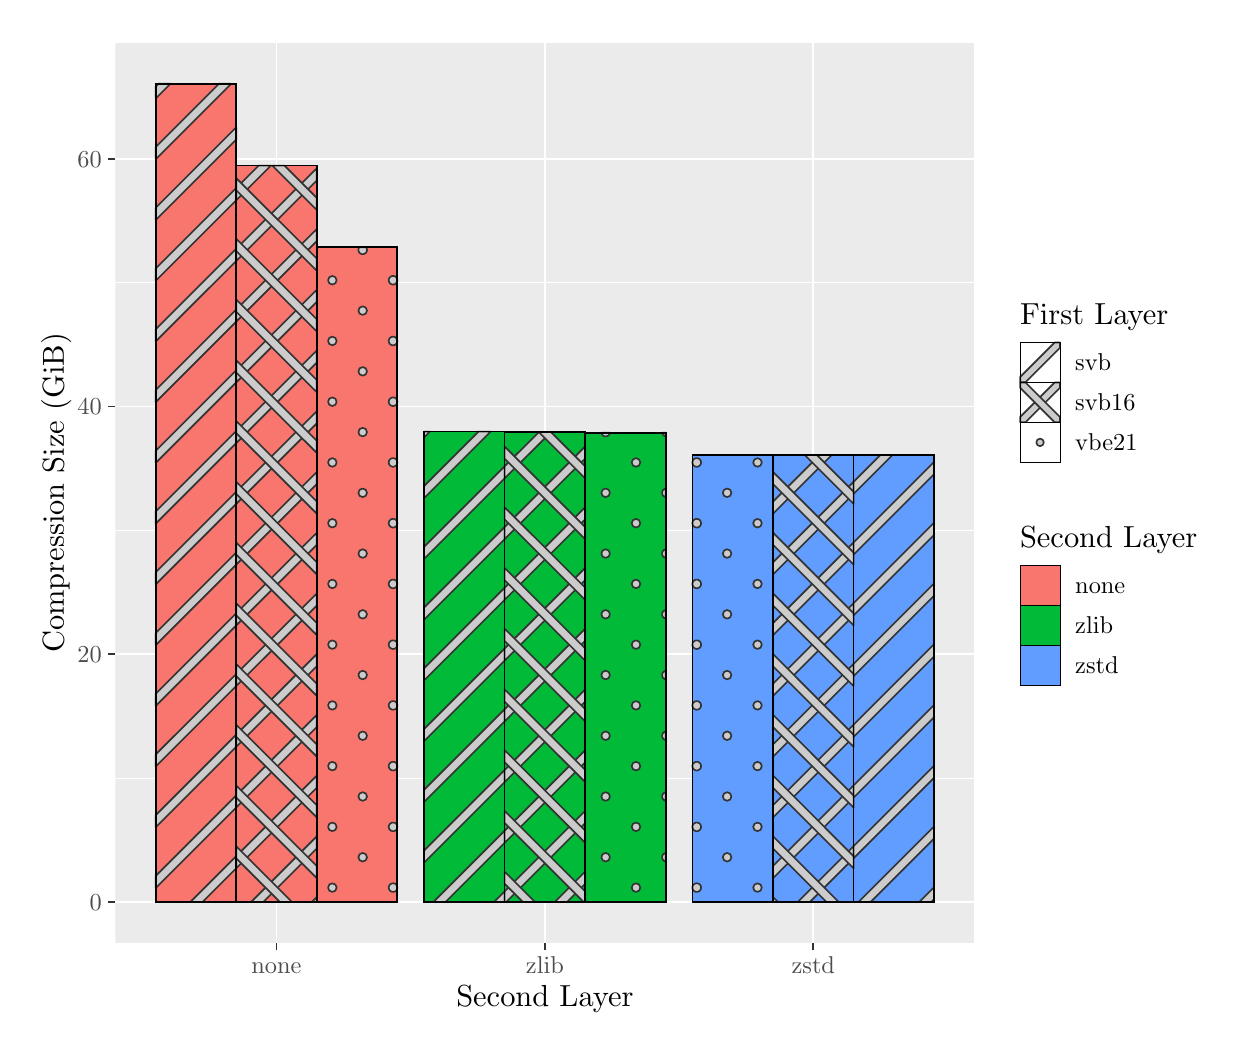
\begin{tikzpicture}[x=1pt,y=1pt]
\definecolor{fillColor}{RGB}{255,255,255}
\path[use as bounding box,fill=fillColor,fill opacity=0.00] (0,0) rectangle (433.62,361.35);
\begin{scope}
\path[clip] (  0.00,  0.00) rectangle (433.62,361.35);
\definecolor{drawColor}{RGB}{255,255,255}
\definecolor{fillColor}{RGB}{255,255,255}

\path[draw=drawColor,line width= 0.6pt,line join=round,line cap=round,fill=fillColor] (  0.00,  0.00) rectangle (433.62,361.35);
\end{scope}
\begin{scope}
\path[clip] ( 31.71, 30.69) rectangle (342.09,355.85);
\definecolor{fillColor}{gray}{0.92}

\path[fill=fillColor] ( 31.71, 30.69) rectangle (342.09,355.85);
\definecolor{drawColor}{RGB}{255,255,255}

\path[draw=drawColor,line width= 0.3pt,line join=round] ( 31.71, 90.22) --
	(342.09, 90.22);

\path[draw=drawColor,line width= 0.3pt,line join=round] ( 31.71,179.73) --
	(342.09,179.73);

\path[draw=drawColor,line width= 0.3pt,line join=round] ( 31.71,269.23) --
	(342.09,269.23);

\path[draw=drawColor,line width= 0.6pt,line join=round] ( 31.71, 45.47) --
	(342.09, 45.47);

\path[draw=drawColor,line width= 0.6pt,line join=round] ( 31.71,134.97) --
	(342.09,134.97);

\path[draw=drawColor,line width= 0.6pt,line join=round] ( 31.71,224.48) --
	(342.09,224.48);

\path[draw=drawColor,line width= 0.6pt,line join=round] ( 31.71,313.99) --
	(342.09,313.99);

\path[draw=drawColor,line width= 0.6pt,line join=round] ( 89.91, 30.69) --
	( 89.91,355.85);

\path[draw=drawColor,line width= 0.6pt,line join=round] (186.90, 30.69) --
	(186.90,355.85);

\path[draw=drawColor,line width= 0.6pt,line join=round] (283.89, 30.69) --
	(283.89,355.85);
\definecolor{fillColor}{RGB}{248,118,109}

\path[fill=fillColor] ( 46.26, 45.47) rectangle ( 75.36,341.07);

\path[fill=fillColor] ( 75.36, 45.47) rectangle (104.46,311.51);

\path[fill=fillColor] (104.46, 45.47) rectangle (133.56,282.00);
\definecolor{fillColor}{RGB}{97,156,255}

\path[fill=fillColor] (240.25, 45.47) rectangle (269.35,206.99);

\path[fill=fillColor] (269.35, 45.47) rectangle (298.44,206.97);

\path[fill=fillColor] (298.44, 45.47) rectangle (327.54,206.97);
\definecolor{fillColor}{RGB}{0,186,56}

\path[fill=fillColor] (143.25, 45.47) rectangle (172.35,215.38);

\path[fill=fillColor] (172.35, 45.47) rectangle (201.45,215.21);

\path[fill=fillColor] (201.45, 45.47) rectangle (230.55,214.96);
\definecolor{drawColor}{gray}{0.20}
\definecolor{fillColor}{gray}{0.80}

\path[draw=drawColor,line width= 0.6pt,line join=round,line cap=rect,fill=fillColor] ( 58.85, 45.47) --
	( 75.36, 61.97) --
	( 75.36, 57.58) --
	( 63.24, 45.47) --
	( 58.85, 45.47) --
	cycle;

\path[draw=drawColor,line width= 0.6pt,line join=round,line cap=rect,fill=fillColor] ( 46.26, 54.82) --
	( 75.36, 83.92) --
	( 75.36, 79.53) --
	( 46.26, 50.43) --
	( 46.26, 54.82) --
	cycle;

\path[draw=drawColor,line width= 0.6pt,line join=round,line cap=rect,fill=fillColor] ( 46.26, 76.77) --
	( 75.36,105.87) --
	( 75.36,101.48) --
	( 46.26, 72.38) --
	( 46.26, 76.77) --
	cycle;

\path[draw=drawColor,line width= 0.6pt,line join=round,line cap=rect,fill=fillColor] ( 46.26, 98.72) --
	( 75.36,127.81) --
	( 75.36,123.43) --
	( 46.26, 94.33) --
	( 46.26, 98.72) --
	cycle;

\path[draw=drawColor,line width= 0.6pt,line join=round,line cap=rect,fill=fillColor] ( 46.26,120.66) --
	( 75.36,149.76) --
	( 75.36,145.37) --
	( 46.26,116.27) --
	( 46.26,120.66) --
	cycle;

\path[draw=drawColor,line width= 0.6pt,line join=round,line cap=rect,fill=fillColor] ( 46.26,142.61) --
	( 75.36,171.71) --
	( 75.36,167.32) --
	( 46.26,138.22) --
	( 46.26,142.61) --
	cycle;

\path[draw=drawColor,line width= 0.6pt,line join=round,line cap=rect,fill=fillColor] ( 46.26,164.56) --
	( 75.36,193.66) --
	( 75.36,189.27) --
	( 46.26,160.17) --
	( 46.26,164.56) --
	cycle;

\path[draw=drawColor,line width= 0.6pt,line join=round,line cap=rect,fill=fillColor] ( 46.26,186.50) --
	( 75.36,215.60) --
	( 75.36,211.21) --
	( 46.26,182.12) --
	( 46.26,186.50) --
	cycle;

\path[draw=drawColor,line width= 0.6pt,line join=round,line cap=rect,fill=fillColor] ( 46.26,208.45) --
	( 75.36,237.55) --
	( 75.36,233.16) --
	( 46.26,204.06) --
	( 46.26,208.45) --
	cycle;

\path[draw=drawColor,line width= 0.6pt,line join=round,line cap=rect,fill=fillColor] ( 46.26,230.40) --
	( 75.36,259.50) --
	( 75.36,255.11) --
	( 46.26,226.01) --
	( 46.26,230.40) --
	cycle;

\path[draw=drawColor,line width= 0.6pt,line join=round,line cap=rect,fill=fillColor] ( 46.26,252.35) --
	( 75.36,281.44) --
	( 75.36,277.05) --
	( 46.26,247.96) --
	( 46.26,252.35) --
	cycle;

\path[draw=drawColor,line width= 0.6pt,line join=round,line cap=rect,fill=fillColor] ( 46.26,274.29) --
	( 75.36,303.39) --
	( 75.36,299.00) --
	( 46.26,269.90) --
	( 46.26,274.29) --
	cycle;

\path[draw=drawColor,line width= 0.6pt,line join=round,line cap=rect,fill=fillColor] ( 46.26,296.24) --
	( 75.36,325.34) --
	( 75.36,320.95) --
	( 46.26,291.85) --
	( 46.26,296.24) --
	cycle;

\path[draw=drawColor,line width= 0.6pt,line join=round,line cap=rect,fill=fillColor] ( 46.26,318.19) --
	( 69.14,341.07) --
	( 73.53,341.07) --
	( 46.26,313.80) --
	( 46.26,318.19) --
	cycle;

\path[draw=drawColor,line width= 0.6pt,line join=round,line cap=rect,fill=fillColor] ( 46.26,340.13) --
	( 47.20,341.07) --
	( 51.59,341.07) --
	( 46.26,335.74) --
	( 46.26,340.13) --
	cycle;

\path[draw=drawColor,line width= 0.6pt,line join=round,line cap=rect,fill=fillColor] (102.75, 45.47) --
	(104.46, 47.18) --
	(104.46, 45.47) --
	(102.75, 45.47) --
	cycle;

\path[draw=drawColor,line width= 0.6pt,line join=round,line cap=rect,fill=fillColor] ( 80.80, 45.47) --
	(104.46, 69.12) --
	(104.46, 64.73) --
	( 85.19, 45.47) --
	( 80.80, 45.47) --
	cycle;

\path[draw=drawColor,line width= 0.6pt,line join=round,line cap=rect,fill=fillColor] ( 75.36, 61.97) --
	(104.46, 91.07) --
	(104.46, 86.68) --
	( 75.36, 57.58) --
	( 75.36, 61.97) --
	cycle;

\path[draw=drawColor,line width= 0.6pt,line join=round,line cap=rect,fill=fillColor] ( 75.36, 83.92) --
	(104.46,113.02) --
	(104.46,108.63) --
	( 75.36, 79.53) --
	( 75.36, 83.92) --
	cycle;

\path[draw=drawColor,line width= 0.6pt,line join=round,line cap=rect,fill=fillColor] ( 75.36,105.87) --
	(104.46,134.97) --
	(104.46,130.58) --
	( 75.36,101.48) --
	( 75.36,105.87) --
	cycle;

\path[draw=drawColor,line width= 0.6pt,line join=round,line cap=rect,fill=fillColor] ( 75.36,127.81) --
	(104.46,156.91) --
	(104.46,152.52) --
	( 75.36,123.43) --
	( 75.36,127.81) --
	cycle;

\path[draw=drawColor,line width= 0.6pt,line join=round,line cap=rect,fill=fillColor] ( 75.36,149.76) --
	(104.46,178.86) --
	(104.46,174.47) --
	( 75.36,145.37) --
	( 75.36,149.76) --
	cycle;

\path[draw=drawColor,line width= 0.6pt,line join=round,line cap=rect,fill=fillColor] ( 75.36,171.71) --
	(104.46,200.81) --
	(104.46,196.42) --
	( 75.36,167.32) --
	( 75.36,171.71) --
	cycle;

\path[draw=drawColor,line width= 0.6pt,line join=round,line cap=rect,fill=fillColor] ( 75.36,193.66) --
	(104.46,222.75) --
	(104.46,218.36) --
	( 75.36,189.27) --
	( 75.36,193.66) --
	cycle;

\path[draw=drawColor,line width= 0.6pt,line join=round,line cap=rect,fill=fillColor] ( 75.36,215.60) --
	(104.46,244.70) --
	(104.46,240.31) --
	( 75.36,211.21) --
	( 75.36,215.60) --
	cycle;

\path[draw=drawColor,line width= 0.6pt,line join=round,line cap=rect,fill=fillColor] ( 75.36,237.55) --
	(104.46,266.65) --
	(104.46,262.26) --
	( 75.36,233.16) --
	( 75.36,237.55) --
	cycle;

\path[draw=drawColor,line width= 0.6pt,line join=round,line cap=rect,fill=fillColor] ( 75.36,259.50) --
	(104.46,288.59) --
	(104.46,284.21) --
	( 75.36,255.11) --
	( 75.36,259.50) --
	cycle;

\path[draw=drawColor,line width= 0.6pt,line join=round,line cap=rect,fill=fillColor] ( 75.36,281.44) --
	(104.46,310.54) --
	(104.46,306.15) --
	( 75.36,277.05) --
	( 75.36,281.44) --
	cycle;

\path[draw=drawColor,line width= 0.6pt,line join=round,line cap=rect,fill=fillColor] ( 75.36,303.39) --
	( 83.48,311.51) --
	( 87.87,311.51) --
	( 75.36,299.00) --
	( 75.36,303.39) --
	cycle;

\path[draw=drawColor,line width= 0.6pt,line join=round,line cap=rect,fill=fillColor] ( 75.36, 65.59) --
	( 95.48, 45.47) --
	( 91.09, 45.47) --
	( 75.36, 61.20) --
	( 75.36, 65.59) --
	cycle;

\path[draw=drawColor,line width= 0.6pt,line join=round,line cap=rect,fill=fillColor] ( 75.36, 87.53) --
	(104.46, 58.44) --
	(104.46, 54.05) --
	( 75.36, 83.14) --
	( 75.36, 87.53) --
	cycle;

\path[draw=drawColor,line width= 0.6pt,line join=round,line cap=rect,fill=fillColor] ( 75.36,109.48) --
	(104.46, 80.38) --
	(104.46, 75.99) --
	( 75.36,105.09) --
	( 75.36,109.48) --
	cycle;

\path[draw=drawColor,line width= 0.6pt,line join=round,line cap=rect,fill=fillColor] ( 75.36,131.43) --
	(104.46,102.33) --
	(104.46, 97.94) --
	( 75.36,127.04) --
	( 75.36,131.43) --
	cycle;

\path[draw=drawColor,line width= 0.6pt,line join=round,line cap=rect,fill=fillColor] ( 75.36,153.38) --
	(104.46,124.28) --
	(104.46,119.89) --
	( 75.36,148.99) --
	( 75.36,153.38) --
	cycle;

\path[draw=drawColor,line width= 0.6pt,line join=round,line cap=rect,fill=fillColor] ( 75.36,175.32) --
	(104.46,146.22) --
	(104.46,141.84) --
	( 75.36,170.93) --
	( 75.36,175.32) --
	cycle;

\path[draw=drawColor,line width= 0.6pt,line join=round,line cap=rect,fill=fillColor] ( 75.36,197.27) --
	(104.46,168.17) --
	(104.46,163.78) --
	( 75.36,192.88) --
	( 75.36,197.27) --
	cycle;

\path[draw=drawColor,line width= 0.6pt,line join=round,line cap=rect,fill=fillColor] ( 75.36,219.22) --
	(104.46,190.12) --
	(104.46,185.73) --
	( 75.36,214.83) --
	( 75.36,219.22) --
	cycle;

\path[draw=drawColor,line width= 0.6pt,line join=round,line cap=rect,fill=fillColor] ( 75.36,241.16) --
	(104.46,212.07) --
	(104.46,207.68) --
	( 75.36,236.77) --
	( 75.36,241.16) --
	cycle;

\path[draw=drawColor,line width= 0.6pt,line join=round,line cap=rect,fill=fillColor] ( 75.36,263.11) --
	(104.46,234.01) --
	(104.46,229.62) --
	( 75.36,258.72) --
	( 75.36,263.11) --
	cycle;

\path[draw=drawColor,line width= 0.6pt,line join=round,line cap=rect,fill=fillColor] ( 75.36,285.06) --
	(104.46,255.96) --
	(104.46,251.57) --
	( 75.36,280.67) --
	( 75.36,285.06) --
	cycle;

\path[draw=drawColor,line width= 0.6pt,line join=round,line cap=rect,fill=fillColor] ( 75.36,307.00) --
	(104.46,277.91) --
	(104.46,273.52) --
	( 75.36,302.62) --
	( 75.36,307.00) --
	cycle;

\path[draw=drawColor,line width= 0.6pt,line join=round,line cap=rect,fill=fillColor] ( 92.80,311.51) --
	(104.46,299.85) --
	(104.46,295.46) --
	( 88.41,311.51) --
	( 92.80,311.51) --
	cycle;

\path[draw=drawColor,line width= 0.6pt,line join=round,line cap=round,fill=fillColor] (110.09, 94.51) circle (  1.55);

\path[draw=drawColor,line width= 0.6pt,line join=round,line cap=round,fill=fillColor] (110.09,116.45) circle (  1.55);

\path[draw=drawColor,line width= 0.6pt,line join=round,line cap=round,fill=fillColor] (110.09,138.40) circle (  1.55);

\path[draw=drawColor,line width= 0.6pt,line join=round,line cap=round,fill=fillColor] (110.09,226.19) circle (  1.55);

\path[draw=drawColor,line width= 0.6pt,line join=round,line cap=round,fill=fillColor] (110.09,248.14) circle (  1.55);

\path[draw=drawColor,line width= 0.6pt,line join=round,line cap=round,fill=fillColor] (110.09,160.35) circle (  1.55);

\path[draw=drawColor,line width= 0.6pt,line join=round,line cap=round,fill=fillColor] (110.09,204.24) circle (  1.55);

\path[draw=drawColor,line width= 0.6pt,line join=round,line cap=round,fill=fillColor] (110.09,182.29) circle (  1.55);

\path[draw=drawColor,line width= 0.6pt,line join=round,line cap=round,fill=fillColor] (110.09,270.08) circle (  1.55);

\path[draw=drawColor,line width= 0.6pt,line join=round,line cap=round,fill=fillColor] (110.09, 50.61) circle (  1.55);

\path[draw=drawColor,line width= 0.6pt,line join=round,line cap=round,fill=fillColor] (110.09, 72.56) circle (  1.55);

\path[draw=drawColor,line width= 0.6pt,line join=round,line cap=round,fill=fillColor] (121.06,127.43) circle (  1.55);

\path[draw=drawColor,line width= 0.6pt,line join=round,line cap=round,fill=fillColor] (121.06,149.37) circle (  1.55);

\path[draw=drawColor,line width= 0.6pt,line join=round,line cap=round,fill=fillColor] (121.06,237.16) circle (  1.55);

\path[draw=drawColor,line width= 0.6pt,line join=round,line cap=round,fill=fillColor] (121.06,105.48) circle (  1.55);

\path[draw=drawColor,line width= 0.6pt,line join=round,line cap=round,fill=fillColor] (121.06,171.32) circle (  1.55);

\path[draw=drawColor,line width= 0.6pt,line join=round,line cap=round,fill=fillColor] (121.06,193.27) circle (  1.55);

\path[draw=drawColor,line width= 0.6pt,line join=round,line cap=round,fill=fillColor] (121.06,215.21) circle (  1.55);

\path[draw=drawColor,line width= 0.6pt,line join=round,line cap=round,fill=fillColor] (121.06,259.11) circle (  1.55);

\path[draw=drawColor,line width= 0.6pt,line join=round,line cap=round,fill=fillColor] (121.06, 83.53) circle (  1.55);

\path[draw=drawColor,line width= 0.6pt,line join=round,line cap=round,fill=fillColor] (121.06, 61.59) circle (  1.55);

\path[draw=drawColor,line width= 0.6pt,line join=round,line cap=round,fill=fillColor] (122.30,282.00) --
	(122.34,281.93) --
	(122.40,281.85) --
	(122.44,281.76) --
	(122.48,281.67) --
	(122.52,281.58) --
	(122.55,281.49) --
	(122.57,281.39) --
	(122.59,281.30) --
	(122.61,281.20) --
	(122.61,281.10) --
	(122.61,281.01) --
	(122.61,280.91) --
	(122.59,280.81) --
	(122.57,280.72) --
	(122.55,280.62) --
	(122.52,280.53) --
	(122.48,280.44) --
	(122.44,280.35) --
	(122.40,280.27) --
	(122.34,280.18) --
	(122.29,280.11) --
	(122.22,280.03) --
	(122.16,279.96) --
	(122.09,279.89) --
	(122.01,279.83) --
	(121.93,279.77) --
	(121.85,279.72) --
	(121.76,279.67) --
	(121.68,279.63) --
	(121.59,279.60) --
	(121.49,279.57) --
	(121.40,279.54) --
	(121.30,279.52) --
	(121.21,279.51) --
	(121.11,279.51) --
	(121.01,279.51) --
	(120.91,279.51) --
	(120.82,279.52) --
	(120.72,279.54) --
	(120.63,279.57) --
	(120.53,279.60) --
	(120.44,279.63) --
	(120.36,279.67) --
	(120.27,279.72) --
	(120.19,279.77) --
	(120.11,279.83) --
	(120.03,279.89) --
	(119.96,279.96) --
	(119.90,280.03) --
	(119.83,280.11) --
	(119.78,280.18) --
	(119.72,280.27) --
	(119.68,280.35) --
	(119.64,280.44) --
	(119.60,280.53) --
	(119.57,280.62) --
	(119.55,280.72) --
	(119.53,280.81) --
	(119.52,280.91) --
	(119.51,281.01) --
	(119.51,281.10) --
	(119.52,281.20) --
	(119.53,281.30) --
	(119.55,281.39) --
	(119.57,281.49) --
	(119.60,281.58) --
	(119.64,281.67) --
	(119.68,281.76) --
	(119.72,281.85) --
	(119.78,281.93) --
	(119.83,282.00) --
	(122.30,282.00) --
	cycle;

\path[draw=drawColor,line width= 0.6pt,line join=round,line cap=round,fill=fillColor] (133.56,116.15) --
	(133.55,116.11) --
	(133.52,116.02) --
	(133.49,115.93) --
	(133.46,115.84) --
	(133.42,115.75) --
	(133.37,115.66) --
	(133.32,115.58) --
	(133.26,115.50) --
	(133.20,115.43) --
	(133.13,115.36) --
	(133.06,115.29) --
	(132.98,115.23) --
	(132.91,115.17) --
	(132.82,115.12) --
	(132.74,115.07) --
	(132.65,115.03) --
	(132.56,114.99) --
	(132.47,114.96) --
	(132.37,114.94) --
	(132.28,114.92) --
	(132.18,114.91) --
	(132.08,114.90) --
	(131.99,114.90) --
	(131.89,114.91) --
	(131.79,114.92) --
	(131.70,114.94) --
	(131.60,114.96) --
	(131.51,114.99) --
	(131.42,115.03) --
	(131.33,115.07) --
	(131.24,115.12) --
	(131.16,115.17) --
	(131.08,115.23) --
	(131.01,115.29) --
	(130.94,115.36) --
	(130.87,115.43) --
	(130.81,115.50) --
	(130.75,115.58) --
	(130.70,115.66) --
	(130.65,115.75) --
	(130.61,115.84) --
	(130.57,115.93) --
	(130.54,116.02) --
	(130.52,116.11) --
	(130.50,116.21) --
	(130.49,116.31) --
	(130.48,116.40) --
	(130.48,116.50) --
	(130.49,116.60) --
	(130.50,116.70) --
	(130.52,116.79) --
	(130.54,116.89) --
	(130.57,116.98) --
	(130.61,117.07) --
	(130.65,117.16) --
	(130.70,117.24) --
	(130.75,117.33) --
	(130.81,117.40) --
	(130.87,117.48) --
	(130.94,117.55) --
	(131.01,117.62) --
	(131.08,117.68) --
	(131.16,117.74) --
	(131.24,117.79) --
	(131.33,117.84) --
	(131.42,117.88) --
	(131.51,117.91) --
	(131.60,117.94) --
	(131.70,117.97) --
	(131.79,117.99) --
	(131.89,118.00) --
	(131.99,118.00) --
	(132.08,118.00) --
	(132.18,118.00) --
	(132.28,117.99) --
	(132.37,117.97) --
	(132.47,117.94) --
	(132.56,117.91) --
	(132.65,117.88) --
	(132.74,117.84) --
	(132.82,117.79) --
	(132.91,117.74) --
	(132.98,117.68) --
	(133.06,117.62) --
	(133.13,117.55) --
	(133.20,117.48) --
	(133.26,117.40) --
	(133.32,117.33) --
	(133.37,117.24) --
	(133.42,117.16) --
	(133.46,117.07) --
	(133.49,116.98) --
	(133.52,116.89) --
	(133.55,116.79) --
	(133.56,116.76) --
	(133.56,116.15) --
	cycle;

\path[draw=drawColor,line width= 0.6pt,line join=round,line cap=round,fill=fillColor] (133.56,138.10) --
	(133.55,138.06) --
	(133.52,137.97) --
	(133.49,137.87) --
	(133.46,137.78) --
	(133.42,137.70) --
	(133.37,137.61) --
	(133.32,137.53) --
	(133.26,137.45) --
	(133.20,137.37) --
	(133.13,137.30) --
	(133.06,137.24) --
	(132.98,137.17) --
	(132.91,137.12) --
	(132.82,137.06) --
	(132.74,137.02) --
	(132.65,136.98) --
	(132.56,136.94) --
	(132.47,136.91) --
	(132.37,136.89) --
	(132.28,136.87) --
	(132.18,136.86) --
	(132.08,136.85) --
	(131.99,136.85) --
	(131.89,136.86) --
	(131.79,136.87) --
	(131.70,136.89) --
	(131.60,136.91) --
	(131.51,136.94) --
	(131.42,136.98) --
	(131.33,137.02) --
	(131.24,137.06) --
	(131.16,137.12) --
	(131.08,137.17) --
	(131.01,137.24) --
	(130.94,137.30) --
	(130.87,137.37) --
	(130.81,137.45) --
	(130.75,137.53) --
	(130.70,137.61) --
	(130.65,137.70) --
	(130.61,137.78) --
	(130.57,137.87) --
	(130.54,137.97) --
	(130.52,138.06) --
	(130.50,138.16) --
	(130.49,138.25) --
	(130.48,138.35) --
	(130.48,138.45) --
	(130.49,138.55) --
	(130.50,138.64) --
	(130.52,138.74) --
	(130.54,138.83) --
	(130.57,138.93) --
	(130.61,139.02) --
	(130.65,139.10) --
	(130.70,139.19) --
	(130.75,139.27) --
	(130.81,139.35) --
	(130.87,139.43) --
	(130.94,139.50) --
	(131.01,139.56) --
	(131.08,139.63) --
	(131.16,139.68) --
	(131.24,139.74) --
	(131.33,139.78) --
	(131.42,139.82) --
	(131.51,139.86) --
	(131.60,139.89) --
	(131.70,139.91) --
	(131.79,139.93) --
	(131.89,139.95) --
	(131.99,139.95) --
	(132.08,139.95) --
	(132.18,139.95) --
	(132.28,139.93) --
	(132.37,139.91) --
	(132.47,139.89) --
	(132.56,139.86) --
	(132.65,139.82) --
	(132.74,139.78) --
	(132.82,139.74) --
	(132.91,139.68) --
	(132.98,139.63) --
	(133.06,139.56) --
	(133.13,139.50) --
	(133.20,139.43) --
	(133.26,139.35) --
	(133.32,139.27) --
	(133.37,139.19) --
	(133.42,139.10) --
	(133.46,139.02) --
	(133.49,138.93) --
	(133.52,138.83) --
	(133.55,138.74) --
	(133.56,138.70) --
	(133.56,138.10) --
	cycle;

\path[draw=drawColor,line width= 0.6pt,line join=round,line cap=round,fill=fillColor] (133.56,225.89) --
	(133.55,225.85) --
	(133.52,225.76) --
	(133.49,225.66) --
	(133.46,225.57) --
	(133.42,225.48) --
	(133.37,225.40) --
	(133.32,225.32) --
	(133.26,225.24) --
	(133.20,225.16) --
	(133.13,225.09) --
	(133.06,225.02) --
	(132.98,224.96) --
	(132.91,224.90) --
	(132.82,224.85) --
	(132.74,224.81) --
	(132.65,224.76) --
	(132.56,224.73) --
	(132.47,224.70) --
	(132.37,224.67) --
	(132.28,224.66) --
	(132.18,224.64) --
	(132.08,224.64) --
	(131.99,224.64) --
	(131.89,224.64) --
	(131.79,224.66) --
	(131.70,224.67) --
	(131.60,224.70) --
	(131.51,224.73) --
	(131.42,224.76) --
	(131.33,224.81) --
	(131.24,224.85) --
	(131.16,224.90) --
	(131.08,224.96) --
	(131.01,225.02) --
	(130.94,225.09) --
	(130.87,225.16) --
	(130.81,225.24) --
	(130.75,225.32) --
	(130.70,225.40) --
	(130.65,225.48) --
	(130.61,225.57) --
	(130.57,225.66) --
	(130.54,225.76) --
	(130.52,225.85) --
	(130.50,225.95) --
	(130.49,226.04) --
	(130.48,226.14) --
	(130.48,226.24) --
	(130.49,226.33) --
	(130.50,226.43) --
	(130.52,226.53) --
	(130.54,226.62) --
	(130.57,226.71) --
	(130.61,226.80) --
	(130.65,226.89) --
	(130.70,226.98) --
	(130.75,227.06) --
	(130.81,227.14) --
	(130.87,227.21) --
	(130.94,227.29) --
	(131.01,227.35) --
	(131.08,227.41) --
	(131.16,227.47) --
	(131.24,227.52) --
	(131.33,227.57) --
	(131.42,227.61) --
	(131.51,227.65) --
	(131.60,227.68) --
	(131.70,227.70) --
	(131.79,227.72) --
	(131.89,227.73) --
	(131.99,227.74) --
	(132.08,227.74) --
	(132.18,227.73) --
	(132.28,227.72) --
	(132.37,227.70) --
	(132.47,227.68) --
	(132.56,227.65) --
	(132.65,227.61) --
	(132.74,227.57) --
	(132.82,227.52) --
	(132.91,227.47) --
	(132.98,227.41) --
	(133.06,227.35) --
	(133.13,227.29) --
	(133.20,227.21) --
	(133.26,227.14) --
	(133.32,227.06) --
	(133.37,226.98) --
	(133.42,226.89) --
	(133.46,226.80) --
	(133.49,226.71) --
	(133.52,226.62) --
	(133.55,226.53) --
	(133.56,226.49) --
	(133.56,225.89) --
	cycle;

\path[draw=drawColor,line width= 0.6pt,line join=round,line cap=round,fill=fillColor] (133.56,160.04) --
	(133.55,160.01) --
	(133.52,159.91) --
	(133.49,159.82) --
	(133.46,159.73) --
	(133.42,159.64) --
	(133.37,159.56) --
	(133.32,159.47) --
	(133.26,159.40) --
	(133.20,159.32) --
	(133.13,159.25) --
	(133.06,159.18) --
	(132.98,159.12) --
	(132.91,159.06) --
	(132.82,159.01) --
	(132.74,158.96) --
	(132.65,158.92) --
	(132.56,158.89) --
	(132.47,158.86) --
	(132.37,158.83) --
	(132.28,158.81) --
	(132.18,158.80) --
	(132.08,158.80) --
	(131.99,158.80) --
	(131.89,158.80) --
	(131.79,158.81) --
	(131.70,158.83) --
	(131.60,158.86) --
	(131.51,158.89) --
	(131.42,158.92) --
	(131.33,158.96) --
	(131.24,159.01) --
	(131.16,159.06) --
	(131.08,159.12) --
	(131.01,159.18) --
	(130.94,159.25) --
	(130.87,159.32) --
	(130.81,159.40) --
	(130.75,159.47) --
	(130.70,159.56) --
	(130.65,159.64) --
	(130.61,159.73) --
	(130.57,159.82) --
	(130.54,159.91) --
	(130.52,160.01) --
	(130.50,160.10) --
	(130.49,160.20) --
	(130.48,160.30) --
	(130.48,160.40) --
	(130.49,160.49) --
	(130.50,160.59) --
	(130.52,160.69) --
	(130.54,160.78) --
	(130.57,160.87) --
	(130.61,160.96) --
	(130.65,161.05) --
	(130.70,161.14) --
	(130.75,161.22) --
	(130.81,161.30) --
	(130.87,161.37) --
	(130.94,161.44) --
	(131.01,161.51) --
	(131.08,161.57) --
	(131.16,161.63) --
	(131.24,161.68) --
	(131.33,161.73) --
	(131.42,161.77) --
	(131.51,161.81) --
	(131.60,161.84) --
	(131.70,161.86) --
	(131.79,161.88) --
	(131.89,161.89) --
	(131.99,161.90) --
	(132.08,161.90) --
	(132.18,161.89) --
	(132.28,161.88) --
	(132.37,161.86) --
	(132.47,161.84) --
	(132.56,161.81) --
	(132.65,161.77) --
	(132.74,161.73) --
	(132.82,161.68) --
	(132.91,161.63) --
	(132.98,161.57) --
	(133.06,161.51) --
	(133.13,161.44) --
	(133.20,161.37) --
	(133.26,161.30) --
	(133.32,161.22) --
	(133.37,161.14) --
	(133.42,161.05) --
	(133.46,160.96) --
	(133.49,160.87) --
	(133.52,160.78) --
	(133.55,160.69) --
	(133.56,160.65) --
	(133.56,160.04) --
	cycle;

\path[draw=drawColor,line width= 0.6pt,line join=round,line cap=round,fill=fillColor] (133.56,247.83) --
	(133.55,247.80) --
	(133.52,247.70) --
	(133.49,247.61) --
	(133.46,247.52) --
	(133.42,247.43) --
	(133.37,247.35) --
	(133.32,247.26) --
	(133.26,247.18) --
	(133.20,247.11) --
	(133.13,247.04) --
	(133.06,246.97) --
	(132.98,246.91) --
	(132.91,246.85) --
	(132.82,246.80) --
	(132.74,246.75) --
	(132.65,246.71) --
	(132.56,246.68) --
	(132.47,246.65) --
	(132.37,246.62) --
	(132.28,246.60) --
	(132.18,246.59) --
	(132.08,246.58) --
	(131.99,246.58) --
	(131.89,246.59) --
	(131.79,246.60) --
	(131.70,246.62) --
	(131.60,246.65) --
	(131.51,246.68) --
	(131.42,246.71) --
	(131.33,246.75) --
	(131.24,246.80) --
	(131.16,246.85) --
	(131.08,246.91) --
	(131.01,246.97) --
	(130.94,247.04) --
	(130.87,247.11) --
	(130.81,247.18) --
	(130.75,247.26) --
	(130.70,247.35) --
	(130.65,247.43) --
	(130.61,247.52) --
	(130.57,247.61) --
	(130.54,247.70) --
	(130.52,247.80) --
	(130.50,247.89) --
	(130.49,247.99) --
	(130.48,248.09) --
	(130.48,248.18) --
	(130.49,248.28) --
	(130.50,248.38) --
	(130.52,248.47) --
	(130.54,248.57) --
	(130.57,248.66) --
	(130.61,248.75) --
	(130.65,248.84) --
	(130.70,248.93) --
	(130.75,249.01) --
	(130.81,249.09) --
	(130.87,249.16) --
	(130.94,249.23) --
	(131.01,249.30) --
	(131.08,249.36) --
	(131.16,249.42) --
	(131.24,249.47) --
	(131.33,249.52) --
	(131.42,249.56) --
	(131.51,249.60) --
	(131.60,249.63) --
	(131.70,249.65) --
	(131.79,249.67) --
	(131.89,249.68) --
	(131.99,249.69) --
	(132.08,249.69) --
	(132.18,249.68) --
	(132.28,249.67) --
	(132.37,249.65) --
	(132.47,249.63) --
	(132.56,249.60) --
	(132.65,249.56) --
	(132.74,249.52) --
	(132.82,249.47) --
	(132.91,249.42) --
	(132.98,249.36) --
	(133.06,249.30) --
	(133.13,249.23) --
	(133.20,249.16) --
	(133.26,249.09) --
	(133.32,249.01) --
	(133.37,248.93) --
	(133.42,248.84) --
	(133.46,248.75) --
	(133.49,248.66) --
	(133.52,248.57) --
	(133.55,248.47) --
	(133.56,248.44) --
	(133.56,247.83) --
	cycle;

\path[draw=drawColor,line width= 0.6pt,line join=round,line cap=round,fill=fillColor] (133.56, 72.26) --
	(133.55, 72.22) --
	(133.52, 72.13) --
	(133.49, 72.03) --
	(133.46, 71.94) --
	(133.42, 71.85) --
	(133.37, 71.77) --
	(133.32, 71.69) --
	(133.26, 71.61) --
	(133.20, 71.53) --
	(133.13, 71.46) --
	(133.06, 71.39) --
	(132.98, 71.33) --
	(132.91, 71.28) --
	(132.82, 71.22) --
	(132.74, 71.18) --
	(132.65, 71.13) --
	(132.56, 71.10) --
	(132.47, 71.07) --
	(132.37, 71.04) --
	(132.28, 71.03) --
	(132.18, 71.01) --
	(132.08, 71.01) --
	(131.99, 71.01) --
	(131.89, 71.01) --
	(131.79, 71.03) --
	(131.70, 71.04) --
	(131.60, 71.07) --
	(131.51, 71.10) --
	(131.42, 71.13) --
	(131.33, 71.18) --
	(131.24, 71.22) --
	(131.16, 71.28) --
	(131.08, 71.33) --
	(131.01, 71.39) --
	(130.94, 71.46) --
	(130.87, 71.53) --
	(130.81, 71.61) --
	(130.75, 71.69) --
	(130.70, 71.77) --
	(130.65, 71.85) --
	(130.61, 71.94) --
	(130.57, 72.03) --
	(130.54, 72.13) --
	(130.52, 72.22) --
	(130.50, 72.32) --
	(130.49, 72.41) --
	(130.48, 72.51) --
	(130.48, 72.61) --
	(130.49, 72.71) --
	(130.50, 72.80) --
	(130.52, 72.90) --
	(130.54, 72.99) --
	(130.57, 73.08) --
	(130.61, 73.18) --
	(130.65, 73.26) --
	(130.70, 73.35) --
	(130.75, 73.43) --
	(130.81, 73.51) --
	(130.87, 73.59) --
	(130.94, 73.66) --
	(131.01, 73.72) --
	(131.08, 73.79) --
	(131.16, 73.84) --
	(131.24, 73.89) --
	(131.33, 73.94) --
	(131.42, 73.98) --
	(131.51, 74.02) --
	(131.60, 74.05) --
	(131.70, 74.07) --
	(131.79, 74.09) --
	(131.89, 74.10) --
	(131.99, 74.11) --
	(132.08, 74.11) --
	(132.18, 74.10) --
	(132.28, 74.09) --
	(132.37, 74.07) --
	(132.47, 74.05) --
	(132.56, 74.02) --
	(132.65, 73.98) --
	(132.74, 73.94) --
	(132.82, 73.89) --
	(132.91, 73.84) --
	(132.98, 73.79) --
	(133.06, 73.72) --
	(133.13, 73.66) --
	(133.20, 73.59) --
	(133.26, 73.51) --
	(133.32, 73.43) --
	(133.37, 73.35) --
	(133.42, 73.26) --
	(133.46, 73.18) --
	(133.49, 73.08) --
	(133.52, 72.99) --
	(133.55, 72.90) --
	(133.56, 72.86) --
	(133.56, 72.26) --
	cycle;

\path[draw=drawColor,line width= 0.6pt,line join=round,line cap=round,fill=fillColor] (133.56,181.99) --
	(133.55,181.96) --
	(133.52,181.86) --
	(133.49,181.77) --
	(133.46,181.68) --
	(133.42,181.59) --
	(133.37,181.50) --
	(133.32,181.42) --
	(133.26,181.34) --
	(133.20,181.27) --
	(133.13,181.20) --
	(133.06,181.13) --
	(132.98,181.07) --
	(132.91,181.01) --
	(132.82,180.96) --
	(132.74,180.91) --
	(132.65,180.87) --
	(132.56,180.83) --
	(132.47,180.80) --
	(132.37,180.78) --
	(132.28,180.76) --
	(132.18,180.75) --
	(132.08,180.74) --
	(131.99,180.74) --
	(131.89,180.75) --
	(131.79,180.76) --
	(131.70,180.78) --
	(131.60,180.80) --
	(131.51,180.83) --
	(131.42,180.87) --
	(131.33,180.91) --
	(131.24,180.96) --
	(131.16,181.01) --
	(131.08,181.07) --
	(131.01,181.13) --
	(130.94,181.20) --
	(130.87,181.27) --
	(130.81,181.34) --
	(130.75,181.42) --
	(130.70,181.50) --
	(130.65,181.59) --
	(130.61,181.68) --
	(130.57,181.77) --
	(130.54,181.86) --
	(130.52,181.96) --
	(130.50,182.05) --
	(130.49,182.15) --
	(130.48,182.25) --
	(130.48,182.34) --
	(130.49,182.44) --
	(130.50,182.54) --
	(130.52,182.63) --
	(130.54,182.73) --
	(130.57,182.82) --
	(130.61,182.91) --
	(130.65,183.00) --
	(130.70,183.08) --
	(130.75,183.17) --
	(130.81,183.25) --
	(130.87,183.32) --
	(130.94,183.39) --
	(131.01,183.46) --
	(131.08,183.52) --
	(131.16,183.58) --
	(131.24,183.63) --
	(131.33,183.68) --
	(131.42,183.72) --
	(131.51,183.75) --
	(131.60,183.78) --
	(131.70,183.81) --
	(131.79,183.83) --
	(131.89,183.84) --
	(131.99,183.85) --
	(132.08,183.85) --
	(132.18,183.84) --
	(132.28,183.83) --
	(132.37,183.81) --
	(132.47,183.78) --
	(132.56,183.75) --
	(132.65,183.72) --
	(132.74,183.68) --
	(132.82,183.63) --
	(132.91,183.58) --
	(132.98,183.52) --
	(133.06,183.46) --
	(133.13,183.39) --
	(133.20,183.32) --
	(133.26,183.25) --
	(133.32,183.17) --
	(133.37,183.08) --
	(133.42,183.00) --
	(133.46,182.91) --
	(133.49,182.82) --
	(133.52,182.73) --
	(133.55,182.63) --
	(133.56,182.60) --
	(133.56,181.99) --
	cycle;

\path[draw=drawColor,line width= 0.6pt,line join=round,line cap=round,fill=fillColor] (133.56,203.94) --
	(133.55,203.90) --
	(133.52,203.81) --
	(133.49,203.72) --
	(133.46,203.63) --
	(133.42,203.54) --
	(133.37,203.45) --
	(133.32,203.37) --
	(133.26,203.29) --
	(133.20,203.22) --
	(133.13,203.14) --
	(133.06,203.08) --
	(132.98,203.02) --
	(132.91,202.96) --
	(132.82,202.91) --
	(132.74,202.86) --
	(132.65,202.82) --
	(132.56,202.78) --
	(132.47,202.75) --
	(132.37,202.73) --
	(132.28,202.71) --
	(132.18,202.70) --
	(132.08,202.69) --
	(131.99,202.69) --
	(131.89,202.70) --
	(131.79,202.71) --
	(131.70,202.73) --
	(131.60,202.75) --
	(131.51,202.78) --
	(131.42,202.82) --
	(131.33,202.86) --
	(131.24,202.91) --
	(131.16,202.96) --
	(131.08,203.02) --
	(131.01,203.08) --
	(130.94,203.14) --
	(130.87,203.22) --
	(130.81,203.29) --
	(130.75,203.37) --
	(130.70,203.45) --
	(130.65,203.54) --
	(130.61,203.63) --
	(130.57,203.72) --
	(130.54,203.81) --
	(130.52,203.90) --
	(130.50,204.00) --
	(130.49,204.10) --
	(130.48,204.19) --
	(130.48,204.29) --
	(130.49,204.39) --
	(130.50,204.48) --
	(130.52,204.58) --
	(130.54,204.67) --
	(130.57,204.77) --
	(130.61,204.86) --
	(130.65,204.95) --
	(130.70,205.03) --
	(130.75,205.11) --
	(130.81,205.19) --
	(130.87,205.27) --
	(130.94,205.34) --
	(131.01,205.41) --
	(131.08,205.47) --
	(131.16,205.52) --
	(131.24,205.58) --
	(131.33,205.62) --
	(131.42,205.67) --
	(131.51,205.70) --
	(131.60,205.73) --
	(131.70,205.76) --
	(131.79,205.77) --
	(131.89,205.79) --
	(131.99,205.79) --
	(132.08,205.79) --
	(132.18,205.79) --
	(132.28,205.77) --
	(132.37,205.76) --
	(132.47,205.73) --
	(132.56,205.70) --
	(132.65,205.67) --
	(132.74,205.62) --
	(132.82,205.58) --
	(132.91,205.52) --
	(132.98,205.47) --
	(133.06,205.41) --
	(133.13,205.34) --
	(133.20,205.27) --
	(133.26,205.19) --
	(133.32,205.11) --
	(133.37,205.03) --
	(133.42,204.95) --
	(133.46,204.86) --
	(133.49,204.77) --
	(133.52,204.67) --
	(133.55,204.58) --
	(133.56,204.54) --
	(133.56,203.94) --
	cycle;

\path[draw=drawColor,line width= 0.6pt,line join=round,line cap=round,fill=fillColor] (133.56,269.78) --
	(133.55,269.74) --
	(133.52,269.65) --
	(133.49,269.56) --
	(133.46,269.47) --
	(133.42,269.38) --
	(133.37,269.29) --
	(133.32,269.21) --
	(133.26,269.13) --
	(133.20,269.06) --
	(133.13,268.99) --
	(133.06,268.92) --
	(132.98,268.86) --
	(132.91,268.80) --
	(132.82,268.75) --
	(132.74,268.70) --
	(132.65,268.66) --
	(132.56,268.62) --
	(132.47,268.59) --
	(132.37,268.57) --
	(132.28,268.55) --
	(132.18,268.54) --
	(132.08,268.53) --
	(131.99,268.53) --
	(131.89,268.54) --
	(131.79,268.55) --
	(131.70,268.57) --
	(131.60,268.59) --
	(131.51,268.62) --
	(131.42,268.66) --
	(131.33,268.70) --
	(131.24,268.75) --
	(131.16,268.80) --
	(131.08,268.86) --
	(131.01,268.92) --
	(130.94,268.99) --
	(130.87,269.06) --
	(130.81,269.13) --
	(130.75,269.21) --
	(130.70,269.29) --
	(130.65,269.38) --
	(130.61,269.47) --
	(130.57,269.56) --
	(130.54,269.65) --
	(130.52,269.74) --
	(130.50,269.84) --
	(130.49,269.94) --
	(130.48,270.03) --
	(130.48,270.13) --
	(130.49,270.23) --
	(130.50,270.33) --
	(130.52,270.42) --
	(130.54,270.52) --
	(130.57,270.61) --
	(130.61,270.70) --
	(130.65,270.79) --
	(130.70,270.87) --
	(130.75,270.95) --
	(130.81,271.03) --
	(130.87,271.11) --
	(130.94,271.18) --
	(131.01,271.25) --
	(131.08,271.31) --
	(131.16,271.37) --
	(131.24,271.42) --
	(131.33,271.47) --
	(131.42,271.51) --
	(131.51,271.54) --
	(131.60,271.57) --
	(131.70,271.60) --
	(131.79,271.62) --
	(131.89,271.63) --
	(131.99,271.63) --
	(132.08,271.63) --
	(132.18,271.63) --
	(132.28,271.62) --
	(132.37,271.60) --
	(132.47,271.57) --
	(132.56,271.54) --
	(132.65,271.51) --
	(132.74,271.47) --
	(132.82,271.42) --
	(132.91,271.37) --
	(132.98,271.31) --
	(133.06,271.25) --
	(133.13,271.18) --
	(133.20,271.11) --
	(133.26,271.03) --
	(133.32,270.95) --
	(133.37,270.87) --
	(133.42,270.79) --
	(133.46,270.70) --
	(133.49,270.61) --
	(133.52,270.52) --
	(133.55,270.42) --
	(133.56,270.39) --
	(133.56,269.78) --
	cycle;

\path[draw=drawColor,line width= 0.6pt,line join=round,line cap=round,fill=fillColor] (133.56, 50.31) --
	(133.55, 50.27) --
	(133.52, 50.18) --
	(133.49, 50.09) --
	(133.46, 50.00) --
	(133.42, 49.91) --
	(133.37, 49.82) --
	(133.32, 49.74) --
	(133.26, 49.66) --
	(133.20, 49.59) --
	(133.13, 49.51) --
	(133.06, 49.45) --
	(132.98, 49.39) --
	(132.91, 49.33) --
	(132.82, 49.28) --
	(132.74, 49.23) --
	(132.65, 49.19) --
	(132.56, 49.15) --
	(132.47, 49.12) --
	(132.37, 49.10) --
	(132.28, 49.08) --
	(132.18, 49.07) --
	(132.08, 49.06) --
	(131.99, 49.06) --
	(131.89, 49.07) --
	(131.79, 49.08) --
	(131.70, 49.10) --
	(131.60, 49.12) --
	(131.51, 49.15) --
	(131.42, 49.19) --
	(131.33, 49.23) --
	(131.24, 49.28) --
	(131.16, 49.33) --
	(131.08, 49.39) --
	(131.01, 49.45) --
	(130.94, 49.51) --
	(130.87, 49.59) --
	(130.81, 49.66) --
	(130.75, 49.74) --
	(130.70, 49.82) --
	(130.65, 49.91) --
	(130.61, 50.00) --
	(130.57, 50.09) --
	(130.54, 50.18) --
	(130.52, 50.27) --
	(130.50, 50.37) --
	(130.49, 50.47) --
	(130.48, 50.56) --
	(130.48, 50.66) --
	(130.49, 50.76) --
	(130.50, 50.85) --
	(130.52, 50.95) --
	(130.54, 51.04) --
	(130.57, 51.14) --
	(130.61, 51.23) --
	(130.65, 51.32) --
	(130.70, 51.40) --
	(130.75, 51.48) --
	(130.81, 51.56) --
	(130.87, 51.64) --
	(130.94, 51.71) --
	(131.01, 51.78) --
	(131.08, 51.84) --
	(131.16, 51.90) --
	(131.24, 51.95) --
	(131.33, 51.99) --
	(131.42, 52.04) --
	(131.51, 52.07) --
	(131.60, 52.10) --
	(131.70, 52.13) --
	(131.79, 52.14) --
	(131.89, 52.16) --
	(131.99, 52.16) --
	(132.08, 52.16) --
	(132.18, 52.16) --
	(132.28, 52.14) --
	(132.37, 52.13) --
	(132.47, 52.10) --
	(132.56, 52.07) --
	(132.65, 52.04) --
	(132.74, 51.99) --
	(132.82, 51.95) --
	(132.91, 51.90) --
	(132.98, 51.84) --
	(133.06, 51.78) --
	(133.13, 51.71) --
	(133.20, 51.64) --
	(133.26, 51.56) --
	(133.32, 51.48) --
	(133.37, 51.40) --
	(133.42, 51.32) --
	(133.46, 51.23) --
	(133.49, 51.14) --
	(133.52, 51.04) --
	(133.55, 50.95) --
	(133.56, 50.91) --
	(133.56, 50.31) --
	cycle;

\path[draw=drawColor,line width= 0.6pt,line join=round,line cap=round,fill=fillColor] (133.56, 94.20) --
	(133.55, 94.17) --
	(133.52, 94.07) --
	(133.49, 93.98) --
	(133.46, 93.89) --
	(133.42, 93.80) --
	(133.37, 93.72) --
	(133.32, 93.63) --
	(133.26, 93.55) --
	(133.20, 93.48) --
	(133.13, 93.41) --
	(133.06, 93.34) --
	(132.98, 93.28) --
	(132.91, 93.22) --
	(132.82, 93.17) --
	(132.74, 93.12) --
	(132.65, 93.08) --
	(132.56, 93.05) --
	(132.47, 93.02) --
	(132.37, 92.99) --
	(132.28, 92.97) --
	(132.18, 92.96) --
	(132.08, 92.95) --
	(131.99, 92.95) --
	(131.89, 92.96) --
	(131.79, 92.97) --
	(131.70, 92.99) --
	(131.60, 93.02) --
	(131.51, 93.05) --
	(131.42, 93.08) --
	(131.33, 93.12) --
	(131.24, 93.17) --
	(131.16, 93.22) --
	(131.08, 93.28) --
	(131.01, 93.34) --
	(130.94, 93.41) --
	(130.87, 93.48) --
	(130.81, 93.55) --
	(130.75, 93.63) --
	(130.70, 93.72) --
	(130.65, 93.80) --
	(130.61, 93.89) --
	(130.57, 93.98) --
	(130.54, 94.07) --
	(130.52, 94.17) --
	(130.50, 94.26) --
	(130.49, 94.36) --
	(130.48, 94.46) --
	(130.48, 94.55) --
	(130.49, 94.65) --
	(130.50, 94.75) --
	(130.52, 94.84) --
	(130.54, 94.94) --
	(130.57, 95.03) --
	(130.61, 95.12) --
	(130.65, 95.21) --
	(130.70, 95.30) --
	(130.75, 95.38) --
	(130.81, 95.46) --
	(130.87, 95.53) --
	(130.94, 95.60) --
	(131.01, 95.67) --
	(131.08, 95.73) --
	(131.16, 95.79) --
	(131.24, 95.84) --
	(131.33, 95.89) --
	(131.42, 95.93) --
	(131.51, 95.97) --
	(131.60, 96.00) --
	(131.70, 96.02) --
	(131.79, 96.04) --
	(131.89, 96.05) --
	(131.99, 96.06) --
	(132.08, 96.06) --
	(132.18, 96.05) --
	(132.28, 96.04) --
	(132.37, 96.02) --
	(132.47, 96.00) --
	(132.56, 95.97) --
	(132.65, 95.93) --
	(132.74, 95.89) --
	(132.82, 95.84) --
	(132.91, 95.79) --
	(132.98, 95.73) --
	(133.06, 95.67) --
	(133.13, 95.60) --
	(133.20, 95.53) --
	(133.26, 95.46) --
	(133.32, 95.38) --
	(133.37, 95.30) --
	(133.42, 95.21) --
	(133.46, 95.12) --
	(133.49, 95.03) --
	(133.52, 94.94) --
	(133.55, 94.84) --
	(133.56, 94.81) --
	(133.56, 94.20) --
	cycle;

\path[draw=drawColor,line width= 0.6pt,line join=round,line cap=round,fill=fillColor] (252.74, 61.59) circle (  1.55);

\path[draw=drawColor,line width= 0.6pt,line join=round,line cap=round,fill=fillColor] (252.74, 83.53) circle (  1.55);

\path[draw=drawColor,line width= 0.6pt,line join=round,line cap=round,fill=fillColor] (252.74,105.48) circle (  1.55);

\path[draw=drawColor,line width= 0.6pt,line join=round,line cap=round,fill=fillColor] (252.74,171.32) circle (  1.55);

\path[draw=drawColor,line width= 0.6pt,line join=round,line cap=round,fill=fillColor] (252.74,193.27) circle (  1.55);

\path[draw=drawColor,line width= 0.6pt,line join=round,line cap=round,fill=fillColor] (252.74,127.43) circle (  1.55);

\path[draw=drawColor,line width= 0.6pt,line join=round,line cap=round,fill=fillColor] (252.74,149.37) circle (  1.55);

\path[draw=drawColor,line width= 0.6pt,line join=round,line cap=round,fill=fillColor] (263.72, 50.61) circle (  1.55);

\path[draw=drawColor,line width= 0.6pt,line join=round,line cap=round,fill=fillColor] (263.72, 72.56) circle (  1.55);

\path[draw=drawColor,line width= 0.6pt,line join=round,line cap=round,fill=fillColor] (263.72,182.29) circle (  1.55);

\path[draw=drawColor,line width= 0.6pt,line join=round,line cap=round,fill=fillColor] (263.72, 94.51) circle (  1.55);

\path[draw=drawColor,line width= 0.6pt,line join=round,line cap=round,fill=fillColor] (263.72,116.45) circle (  1.55);

\path[draw=drawColor,line width= 0.6pt,line join=round,line cap=round,fill=fillColor] (263.72,138.40) circle (  1.55);

\path[draw=drawColor,line width= 0.6pt,line join=round,line cap=round,fill=fillColor] (263.72,160.35) circle (  1.55);

\path[draw=drawColor,line width= 0.6pt,line join=round,line cap=round,fill=fillColor] (263.72,204.24) circle (  1.55);

\path[draw=drawColor,line width= 0.6pt,line join=round,line cap=round,fill=fillColor] (240.25, 72.86) --
	(240.25, 72.90) --
	(240.28, 72.99) --
	(240.31, 73.08) --
	(240.34, 73.18) --
	(240.39, 73.26) --
	(240.43, 73.35) --
	(240.49, 73.43) --
	(240.54, 73.51) --
	(240.61, 73.59) --
	(240.67, 73.66) --
	(240.74, 73.72) --
	(240.82, 73.79) --
	(240.90, 73.84) --
	(240.98, 73.89) --
	(241.06, 73.94) --
	(241.15, 73.98) --
	(241.24, 74.02) --
	(241.34, 74.05) --
	(241.43, 74.07) --
	(241.53, 74.09) --
	(241.62, 74.10) --
	(241.72, 74.11) --
	(241.82, 74.11) --
	(241.92, 74.10) --
	(242.01, 74.09) --
	(242.11, 74.07) --
	(242.20, 74.05) --
	(242.29, 74.02) --
	(242.39, 73.98) --
	(242.47, 73.94) --
	(242.56, 73.89) --
	(242.64, 73.84) --
	(242.72, 73.79) --
	(242.80, 73.72) --
	(242.87, 73.66) --
	(242.93, 73.59) --
	(243.00, 73.51) --
	(243.05, 73.43) --
	(243.11, 73.35) --
	(243.15, 73.26) --
	(243.19, 73.18) --
	(243.23, 73.08) --
	(243.26, 72.99) --
	(243.28, 72.90) --
	(243.30, 72.80) --
	(243.31, 72.71) --
	(243.32, 72.61) --
	(243.32, 72.51) --
	(243.31, 72.41) --
	(243.30, 72.32) --
	(243.28, 72.22) --
	(243.26, 72.13) --
	(243.23, 72.03) --
	(243.19, 71.94) --
	(243.15, 71.85) --
	(243.11, 71.77) --
	(243.05, 71.69) --
	(243.00, 71.61) --
	(242.93, 71.53) --
	(242.87, 71.46) --
	(242.80, 71.39) --
	(242.72, 71.33) --
	(242.64, 71.28) --
	(242.56, 71.22) --
	(242.47, 71.18) --
	(242.39, 71.13) --
	(242.29, 71.10) --
	(242.20, 71.07) --
	(242.11, 71.04) --
	(242.01, 71.03) --
	(241.92, 71.01) --
	(241.82, 71.01) --
	(241.72, 71.01) --
	(241.62, 71.01) --
	(241.53, 71.03) --
	(241.43, 71.04) --
	(241.34, 71.07) --
	(241.24, 71.10) --
	(241.15, 71.13) --
	(241.06, 71.18) --
	(240.98, 71.22) --
	(240.90, 71.28) --
	(240.82, 71.33) --
	(240.74, 71.39) --
	(240.67, 71.46) --
	(240.61, 71.53) --
	(240.54, 71.61) --
	(240.49, 71.69) --
	(240.43, 71.77) --
	(240.39, 71.85) --
	(240.34, 71.94) --
	(240.31, 72.03) --
	(240.28, 72.13) --
	(240.25, 72.22) --
	(240.25, 72.26) --
	(240.25, 72.86) --
	cycle;

\path[draw=drawColor,line width= 0.6pt,line join=round,line cap=round,fill=fillColor] (240.25,116.76) --
	(240.25,116.79) --
	(240.28,116.89) --
	(240.31,116.98) --
	(240.34,117.07) --
	(240.39,117.16) --
	(240.43,117.24) --
	(240.49,117.33) --
	(240.54,117.40) --
	(240.61,117.48) --
	(240.67,117.55) --
	(240.74,117.62) --
	(240.82,117.68) --
	(240.90,117.74) --
	(240.98,117.79) --
	(241.06,117.84) --
	(241.15,117.88) --
	(241.24,117.91) --
	(241.34,117.94) --
	(241.43,117.97) --
	(241.53,117.99) --
	(241.62,118.00) --
	(241.72,118.00) --
	(241.82,118.00) --
	(241.92,118.00) --
	(242.01,117.99) --
	(242.11,117.97) --
	(242.20,117.94) --
	(242.29,117.91) --
	(242.39,117.88) --
	(242.47,117.84) --
	(242.56,117.79) --
	(242.64,117.74) --
	(242.72,117.68) --
	(242.80,117.62) --
	(242.87,117.55) --
	(242.93,117.48) --
	(243.00,117.40) --
	(243.05,117.33) --
	(243.11,117.24) --
	(243.15,117.16) --
	(243.19,117.07) --
	(243.23,116.98) --
	(243.26,116.89) --
	(243.28,116.79) --
	(243.30,116.70) --
	(243.31,116.60) --
	(243.32,116.50) --
	(243.32,116.40) --
	(243.31,116.31) --
	(243.30,116.21) --
	(243.28,116.11) --
	(243.26,116.02) --
	(243.23,115.93) --
	(243.19,115.84) --
	(243.15,115.75) --
	(243.11,115.66) --
	(243.05,115.58) --
	(243.00,115.50) --
	(242.93,115.43) --
	(242.87,115.36) --
	(242.80,115.29) --
	(242.72,115.23) --
	(242.64,115.17) --
	(242.56,115.12) --
	(242.47,115.07) --
	(242.39,115.03) --
	(242.29,114.99) --
	(242.20,114.96) --
	(242.11,114.94) --
	(242.01,114.92) --
	(241.92,114.91) --
	(241.82,114.90) --
	(241.72,114.90) --
	(241.62,114.91) --
	(241.53,114.92) --
	(241.43,114.94) --
	(241.34,114.96) --
	(241.24,114.99) --
	(241.15,115.03) --
	(241.06,115.07) --
	(240.98,115.12) --
	(240.90,115.17) --
	(240.82,115.23) --
	(240.74,115.29) --
	(240.67,115.36) --
	(240.61,115.43) --
	(240.54,115.50) --
	(240.49,115.58) --
	(240.43,115.66) --
	(240.39,115.75) --
	(240.34,115.84) --
	(240.31,115.93) --
	(240.28,116.02) --
	(240.25,116.11) --
	(240.25,116.15) --
	(240.25,116.76) --
	cycle;

\path[draw=drawColor,line width= 0.6pt,line join=round,line cap=round,fill=fillColor] (240.25,138.70) --
	(240.25,138.74) --
	(240.28,138.83) --
	(240.31,138.93) --
	(240.34,139.02) --
	(240.39,139.10) --
	(240.43,139.19) --
	(240.49,139.27) --
	(240.54,139.35) --
	(240.61,139.43) --
	(240.67,139.50) --
	(240.74,139.56) --
	(240.82,139.63) --
	(240.90,139.68) --
	(240.98,139.74) --
	(241.06,139.78) --
	(241.15,139.82) --
	(241.24,139.86) --
	(241.34,139.89) --
	(241.43,139.91) --
	(241.53,139.93) --
	(241.62,139.95) --
	(241.72,139.95) --
	(241.82,139.95) --
	(241.92,139.95) --
	(242.01,139.93) --
	(242.11,139.91) --
	(242.20,139.89) --
	(242.29,139.86) --
	(242.39,139.82) --
	(242.47,139.78) --
	(242.56,139.74) --
	(242.64,139.68) --
	(242.72,139.63) --
	(242.80,139.56) --
	(242.87,139.50) --
	(242.93,139.43) --
	(243.00,139.35) --
	(243.05,139.27) --
	(243.11,139.19) --
	(243.15,139.10) --
	(243.19,139.02) --
	(243.23,138.93) --
	(243.26,138.83) --
	(243.28,138.74) --
	(243.30,138.64) --
	(243.31,138.55) --
	(243.32,138.45) --
	(243.32,138.35) --
	(243.31,138.25) --
	(243.30,138.16) --
	(243.28,138.06) --
	(243.26,137.97) --
	(243.23,137.87) --
	(243.19,137.78) --
	(243.15,137.70) --
	(243.11,137.61) --
	(243.05,137.53) --
	(243.00,137.45) --
	(242.93,137.37) --
	(242.87,137.30) --
	(242.80,137.24) --
	(242.72,137.17) --
	(242.64,137.12) --
	(242.56,137.06) --
	(242.47,137.02) --
	(242.39,136.98) --
	(242.29,136.94) --
	(242.20,136.91) --
	(242.11,136.89) --
	(242.01,136.87) --
	(241.92,136.86) --
	(241.82,136.85) --
	(241.72,136.85) --
	(241.62,136.86) --
	(241.53,136.87) --
	(241.43,136.89) --
	(241.34,136.91) --
	(241.24,136.94) --
	(241.15,136.98) --
	(241.06,137.02) --
	(240.98,137.06) --
	(240.90,137.12) --
	(240.82,137.17) --
	(240.74,137.24) --
	(240.67,137.30) --
	(240.61,137.37) --
	(240.54,137.45) --
	(240.49,137.53) --
	(240.43,137.61) --
	(240.39,137.70) --
	(240.34,137.78) --
	(240.31,137.87) --
	(240.28,137.97) --
	(240.25,138.06) --
	(240.25,138.10) --
	(240.25,138.70) --
	cycle;

\path[draw=drawColor,line width= 0.6pt,line join=round,line cap=round,fill=fillColor] (240.25,160.65) --
	(240.25,160.69) --
	(240.28,160.78) --
	(240.31,160.87) --
	(240.34,160.96) --
	(240.39,161.05) --
	(240.43,161.14) --
	(240.49,161.22) --
	(240.54,161.30) --
	(240.61,161.37) --
	(240.67,161.44) --
	(240.74,161.51) --
	(240.82,161.57) --
	(240.90,161.63) --
	(240.98,161.68) --
	(241.06,161.73) --
	(241.15,161.77) --
	(241.24,161.81) --
	(241.34,161.84) --
	(241.43,161.86) --
	(241.53,161.88) --
	(241.62,161.89) --
	(241.72,161.90) --
	(241.82,161.90) --
	(241.92,161.89) --
	(242.01,161.88) --
	(242.11,161.86) --
	(242.20,161.84) --
	(242.29,161.81) --
	(242.39,161.77) --
	(242.47,161.73) --
	(242.56,161.68) --
	(242.64,161.63) --
	(242.72,161.57) --
	(242.80,161.51) --
	(242.87,161.44) --
	(242.93,161.37) --
	(243.00,161.30) --
	(243.05,161.22) --
	(243.11,161.14) --
	(243.15,161.05) --
	(243.19,160.96) --
	(243.23,160.87) --
	(243.26,160.78) --
	(243.28,160.69) --
	(243.30,160.59) --
	(243.31,160.49) --
	(243.32,160.40) --
	(243.32,160.30) --
	(243.31,160.20) --
	(243.30,160.10) --
	(243.28,160.01) --
	(243.26,159.91) --
	(243.23,159.82) --
	(243.19,159.73) --
	(243.15,159.64) --
	(243.11,159.56) --
	(243.05,159.47) --
	(243.00,159.40) --
	(242.93,159.32) --
	(242.87,159.25) --
	(242.80,159.18) --
	(242.72,159.12) --
	(242.64,159.06) --
	(242.56,159.01) --
	(242.47,158.96) --
	(242.39,158.92) --
	(242.29,158.89) --
	(242.20,158.86) --
	(242.11,158.83) --
	(242.01,158.81) --
	(241.92,158.80) --
	(241.82,158.80) --
	(241.72,158.80) --
	(241.62,158.80) --
	(241.53,158.81) --
	(241.43,158.83) --
	(241.34,158.86) --
	(241.24,158.89) --
	(241.15,158.92) --
	(241.06,158.96) --
	(240.98,159.01) --
	(240.90,159.06) --
	(240.82,159.12) --
	(240.74,159.18) --
	(240.67,159.25) --
	(240.61,159.32) --
	(240.54,159.40) --
	(240.49,159.47) --
	(240.43,159.56) --
	(240.39,159.64) --
	(240.34,159.73) --
	(240.31,159.82) --
	(240.28,159.91) --
	(240.25,160.01) --
	(240.25,160.04) --
	(240.25,160.65) --
	cycle;

\path[draw=drawColor,line width= 0.6pt,line join=round,line cap=round,fill=fillColor] (240.25,182.60) --
	(240.25,182.63) --
	(240.28,182.73) --
	(240.31,182.82) --
	(240.34,182.91) --
	(240.39,183.00) --
	(240.43,183.08) --
	(240.49,183.17) --
	(240.54,183.25) --
	(240.61,183.32) --
	(240.67,183.39) --
	(240.74,183.46) --
	(240.82,183.52) --
	(240.90,183.58) --
	(240.98,183.63) --
	(241.06,183.68) --
	(241.15,183.72) --
	(241.24,183.75) --
	(241.34,183.78) --
	(241.43,183.81) --
	(241.53,183.83) --
	(241.62,183.84) --
	(241.72,183.85) --
	(241.82,183.85) --
	(241.92,183.84) --
	(242.01,183.83) --
	(242.11,183.81) --
	(242.20,183.78) --
	(242.29,183.75) --
	(242.39,183.72) --
	(242.47,183.68) --
	(242.56,183.63) --
	(242.64,183.58) --
	(242.72,183.52) --
	(242.80,183.46) --
	(242.87,183.39) --
	(242.93,183.32) --
	(243.00,183.25) --
	(243.05,183.17) --
	(243.11,183.08) --
	(243.15,183.00) --
	(243.19,182.91) --
	(243.23,182.82) --
	(243.26,182.73) --
	(243.28,182.63) --
	(243.30,182.54) --
	(243.31,182.44) --
	(243.32,182.34) --
	(243.32,182.25) --
	(243.31,182.15) --
	(243.30,182.05) --
	(243.28,181.96) --
	(243.26,181.86) --
	(243.23,181.77) --
	(243.19,181.68) --
	(243.15,181.59) --
	(243.11,181.50) --
	(243.05,181.42) --
	(243.00,181.34) --
	(242.93,181.27) --
	(242.87,181.20) --
	(242.80,181.13) --
	(242.72,181.07) --
	(242.64,181.01) --
	(242.56,180.96) --
	(242.47,180.91) --
	(242.39,180.87) --
	(242.29,180.83) --
	(242.20,180.80) --
	(242.11,180.78) --
	(242.01,180.76) --
	(241.92,180.75) --
	(241.82,180.74) --
	(241.72,180.74) --
	(241.62,180.75) --
	(241.53,180.76) --
	(241.43,180.78) --
	(241.34,180.80) --
	(241.24,180.83) --
	(241.15,180.87) --
	(241.06,180.91) --
	(240.98,180.96) --
	(240.90,181.01) --
	(240.82,181.07) --
	(240.74,181.13) --
	(240.67,181.20) --
	(240.61,181.27) --
	(240.54,181.34) --
	(240.49,181.42) --
	(240.43,181.50) --
	(240.39,181.59) --
	(240.34,181.68) --
	(240.31,181.77) --
	(240.28,181.86) --
	(240.25,181.96) --
	(240.25,181.99) --
	(240.25,182.60) --
	cycle;

\path[draw=drawColor,line width= 0.6pt,line join=round,line cap=round,fill=fillColor] (240.25,204.54) --
	(240.25,204.58) --
	(240.28,204.67) --
	(240.31,204.77) --
	(240.34,204.86) --
	(240.39,204.95) --
	(240.43,205.03) --
	(240.49,205.11) --
	(240.54,205.19) --
	(240.61,205.27) --
	(240.67,205.34) --
	(240.74,205.41) --
	(240.82,205.47) --
	(240.90,205.52) --
	(240.98,205.58) --
	(241.06,205.62) --
	(241.15,205.67) --
	(241.24,205.70) --
	(241.34,205.73) --
	(241.43,205.76) --
	(241.53,205.77) --
	(241.62,205.79) --
	(241.72,205.79) --
	(241.82,205.79) --
	(241.92,205.79) --
	(242.01,205.77) --
	(242.11,205.76) --
	(242.20,205.73) --
	(242.29,205.70) --
	(242.39,205.67) --
	(242.47,205.62) --
	(242.56,205.58) --
	(242.64,205.52) --
	(242.72,205.47) --
	(242.80,205.41) --
	(242.87,205.34) --
	(242.93,205.27) --
	(243.00,205.19) --
	(243.05,205.11) --
	(243.11,205.03) --
	(243.15,204.95) --
	(243.19,204.86) --
	(243.23,204.77) --
	(243.26,204.67) --
	(243.28,204.58) --
	(243.30,204.48) --
	(243.31,204.39) --
	(243.32,204.29) --
	(243.32,204.19) --
	(243.31,204.10) --
	(243.30,204.00) --
	(243.28,203.90) --
	(243.26,203.81) --
	(243.23,203.72) --
	(243.19,203.63) --
	(243.15,203.54) --
	(243.11,203.45) --
	(243.05,203.37) --
	(243.00,203.29) --
	(242.93,203.22) --
	(242.87,203.14) --
	(242.80,203.08) --
	(242.72,203.02) --
	(242.64,202.96) --
	(242.56,202.91) --
	(242.47,202.86) --
	(242.39,202.82) --
	(242.29,202.78) --
	(242.20,202.75) --
	(242.11,202.73) --
	(242.01,202.71) --
	(241.92,202.70) --
	(241.82,202.69) --
	(241.72,202.69) --
	(241.62,202.70) --
	(241.53,202.71) --
	(241.43,202.73) --
	(241.34,202.75) --
	(241.24,202.78) --
	(241.15,202.82) --
	(241.06,202.86) --
	(240.98,202.91) --
	(240.90,202.96) --
	(240.82,203.02) --
	(240.74,203.08) --
	(240.67,203.14) --
	(240.61,203.22) --
	(240.54,203.29) --
	(240.49,203.37) --
	(240.43,203.45) --
	(240.39,203.54) --
	(240.34,203.63) --
	(240.31,203.72) --
	(240.28,203.81) --
	(240.25,203.90) --
	(240.25,203.94) --
	(240.25,204.54) --
	cycle;

\path[draw=drawColor,line width= 0.6pt,line join=round,line cap=round,fill=fillColor] (240.25, 50.91) --
	(240.25, 50.95) --
	(240.28, 51.04) --
	(240.31, 51.14) --
	(240.34, 51.23) --
	(240.39, 51.32) --
	(240.43, 51.40) --
	(240.49, 51.48) --
	(240.54, 51.56) --
	(240.61, 51.64) --
	(240.67, 51.71) --
	(240.74, 51.78) --
	(240.82, 51.84) --
	(240.90, 51.90) --
	(240.98, 51.95) --
	(241.06, 51.99) --
	(241.15, 52.04) --
	(241.24, 52.07) --
	(241.34, 52.10) --
	(241.43, 52.13) --
	(241.53, 52.14) --
	(241.62, 52.16) --
	(241.72, 52.16) --
	(241.82, 52.16) --
	(241.92, 52.16) --
	(242.01, 52.14) --
	(242.11, 52.13) --
	(242.20, 52.10) --
	(242.29, 52.07) --
	(242.39, 52.04) --
	(242.47, 51.99) --
	(242.56, 51.95) --
	(242.64, 51.90) --
	(242.72, 51.84) --
	(242.80, 51.78) --
	(242.87, 51.71) --
	(242.93, 51.64) --
	(243.00, 51.56) --
	(243.05, 51.48) --
	(243.11, 51.40) --
	(243.15, 51.32) --
	(243.19, 51.23) --
	(243.23, 51.14) --
	(243.26, 51.04) --
	(243.28, 50.95) --
	(243.30, 50.85) --
	(243.31, 50.76) --
	(243.32, 50.66) --
	(243.32, 50.56) --
	(243.31, 50.47) --
	(243.30, 50.37) --
	(243.28, 50.27) --
	(243.26, 50.18) --
	(243.23, 50.09) --
	(243.19, 50.00) --
	(243.15, 49.91) --
	(243.11, 49.82) --
	(243.05, 49.74) --
	(243.00, 49.66) --
	(242.93, 49.59) --
	(242.87, 49.51) --
	(242.80, 49.45) --
	(242.72, 49.39) --
	(242.64, 49.33) --
	(242.56, 49.28) --
	(242.47, 49.23) --
	(242.39, 49.19) --
	(242.29, 49.15) --
	(242.20, 49.12) --
	(242.11, 49.10) --
	(242.01, 49.08) --
	(241.92, 49.07) --
	(241.82, 49.06) --
	(241.72, 49.06) --
	(241.62, 49.07) --
	(241.53, 49.08) --
	(241.43, 49.10) --
	(241.34, 49.12) --
	(241.24, 49.15) --
	(241.15, 49.19) --
	(241.06, 49.23) --
	(240.98, 49.28) --
	(240.90, 49.33) --
	(240.82, 49.39) --
	(240.74, 49.45) --
	(240.67, 49.51) --
	(240.61, 49.59) --
	(240.54, 49.66) --
	(240.49, 49.74) --
	(240.43, 49.82) --
	(240.39, 49.91) --
	(240.34, 50.00) --
	(240.31, 50.09) --
	(240.28, 50.18) --
	(240.25, 50.27) --
	(240.25, 50.31) --
	(240.25, 50.91) --
	cycle;

\path[draw=drawColor,line width= 0.6pt,line join=round,line cap=round,fill=fillColor] (240.25, 94.81) --
	(240.25, 94.84) --
	(240.28, 94.94) --
	(240.31, 95.03) --
	(240.34, 95.12) --
	(240.39, 95.21) --
	(240.43, 95.30) --
	(240.49, 95.38) --
	(240.54, 95.46) --
	(240.61, 95.53) --
	(240.67, 95.60) --
	(240.74, 95.67) --
	(240.82, 95.73) --
	(240.90, 95.79) --
	(240.98, 95.84) --
	(241.06, 95.89) --
	(241.15, 95.93) --
	(241.24, 95.97) --
	(241.34, 96.00) --
	(241.43, 96.02) --
	(241.53, 96.04) --
	(241.62, 96.05) --
	(241.72, 96.06) --
	(241.82, 96.06) --
	(241.92, 96.05) --
	(242.01, 96.04) --
	(242.11, 96.02) --
	(242.20, 96.00) --
	(242.29, 95.97) --
	(242.39, 95.93) --
	(242.47, 95.89) --
	(242.56, 95.84) --
	(242.64, 95.79) --
	(242.72, 95.73) --
	(242.80, 95.67) --
	(242.87, 95.60) --
	(242.93, 95.53) --
	(243.00, 95.46) --
	(243.05, 95.38) --
	(243.11, 95.30) --
	(243.15, 95.21) --
	(243.19, 95.12) --
	(243.23, 95.03) --
	(243.26, 94.94) --
	(243.28, 94.84) --
	(243.30, 94.75) --
	(243.31, 94.65) --
	(243.32, 94.55) --
	(243.32, 94.46) --
	(243.31, 94.36) --
	(243.30, 94.26) --
	(243.28, 94.17) --
	(243.26, 94.07) --
	(243.23, 93.98) --
	(243.19, 93.89) --
	(243.15, 93.80) --
	(243.11, 93.72) --
	(243.05, 93.63) --
	(243.00, 93.55) --
	(242.93, 93.48) --
	(242.87, 93.41) --
	(242.80, 93.34) --
	(242.72, 93.28) --
	(242.64, 93.22) --
	(242.56, 93.17) --
	(242.47, 93.12) --
	(242.39, 93.08) --
	(242.29, 93.05) --
	(242.20, 93.02) --
	(242.11, 92.99) --
	(242.01, 92.97) --
	(241.92, 92.96) --
	(241.82, 92.95) --
	(241.72, 92.95) --
	(241.62, 92.96) --
	(241.53, 92.97) --
	(241.43, 92.99) --
	(241.34, 93.02) --
	(241.24, 93.05) --
	(241.15, 93.08) --
	(241.06, 93.12) --
	(240.98, 93.17) --
	(240.90, 93.22) --
	(240.82, 93.28) --
	(240.74, 93.34) --
	(240.67, 93.41) --
	(240.61, 93.48) --
	(240.54, 93.55) --
	(240.49, 93.63) --
	(240.43, 93.72) --
	(240.39, 93.80) --
	(240.34, 93.89) --
	(240.31, 93.98) --
	(240.28, 94.07) --
	(240.25, 94.17) --
	(240.25, 94.20) --
	(240.25, 94.81) --
	cycle;

\path[draw=drawColor,line width= 0.6pt,line join=round,line cap=rect,fill=fillColor] (278.32, 45.47) --
	(298.44, 65.59) --
	(298.44, 61.20) --
	(282.71, 45.47) --
	(278.32, 45.47) --
	cycle;

\path[draw=drawColor,line width= 0.6pt,line join=round,line cap=rect,fill=fillColor] (269.35, 58.44) --
	(298.44, 87.53) --
	(298.44, 83.14) --
	(269.35, 54.05) --
	(269.35, 58.44) --
	cycle;

\path[draw=drawColor,line width= 0.6pt,line join=round,line cap=rect,fill=fillColor] (269.35, 80.38) --
	(298.44,109.48) --
	(298.44,105.09) --
	(269.35, 75.99) --
	(269.35, 80.38) --
	cycle;

\path[draw=drawColor,line width= 0.6pt,line join=round,line cap=rect,fill=fillColor] (269.35,102.33) --
	(298.44,131.43) --
	(298.44,127.04) --
	(269.35, 97.94) --
	(269.35,102.33) --
	cycle;

\path[draw=drawColor,line width= 0.6pt,line join=round,line cap=rect,fill=fillColor] (269.35,124.28) --
	(298.44,153.38) --
	(298.44,148.99) --
	(269.35,119.89) --
	(269.35,124.28) --
	cycle;

\path[draw=drawColor,line width= 0.6pt,line join=round,line cap=rect,fill=fillColor] (269.35,146.22) --
	(298.44,175.32) --
	(298.44,170.93) --
	(269.35,141.84) --
	(269.35,146.22) --
	cycle;

\path[draw=drawColor,line width= 0.6pt,line join=round,line cap=rect,fill=fillColor] (269.35,168.17) --
	(298.44,197.27) --
	(298.44,192.88) --
	(269.35,163.78) --
	(269.35,168.17) --
	cycle;

\path[draw=drawColor,line width= 0.6pt,line join=round,line cap=rect,fill=fillColor] (269.35,190.12) --
	(286.20,206.97) --
	(290.59,206.97) --
	(269.35,185.73) --
	(269.35,190.12) --
	cycle;

\path[draw=drawColor,line width= 0.6pt,line join=round,line cap=rect,fill=fillColor] (269.35, 47.18) --
	(271.06, 45.47) --
	(269.35, 45.47) --
	(269.35, 47.18) --
	cycle;

\path[draw=drawColor,line width= 0.6pt,line join=round,line cap=rect,fill=fillColor] (269.35, 69.12) --
	(293.00, 45.47) --
	(288.61, 45.47) --
	(269.35, 64.73) --
	(269.35, 69.12) --
	cycle;

\path[draw=drawColor,line width= 0.6pt,line join=round,line cap=rect,fill=fillColor] (269.35, 91.07) --
	(298.44, 61.97) --
	(298.44, 57.58) --
	(269.35, 86.68) --
	(269.35, 91.07) --
	cycle;

\path[draw=drawColor,line width= 0.6pt,line join=round,line cap=rect,fill=fillColor] (269.35,113.02) --
	(298.44, 83.92) --
	(298.44, 79.53) --
	(269.35,108.63) --
	(269.35,113.02) --
	cycle;

\path[draw=drawColor,line width= 0.6pt,line join=round,line cap=rect,fill=fillColor] (269.35,134.97) --
	(298.44,105.87) --
	(298.44,101.48) --
	(269.35,130.58) --
	(269.35,134.97) --
	cycle;

\path[draw=drawColor,line width= 0.6pt,line join=round,line cap=rect,fill=fillColor] (269.35,156.91) --
	(298.44,127.81) --
	(298.44,123.43) --
	(269.35,152.52) --
	(269.35,156.91) --
	cycle;

\path[draw=drawColor,line width= 0.6pt,line join=round,line cap=rect,fill=fillColor] (269.35,178.86) --
	(298.44,149.76) --
	(298.44,145.37) --
	(269.35,174.47) --
	(269.35,178.86) --
	cycle;

\path[draw=drawColor,line width= 0.6pt,line join=round,line cap=rect,fill=fillColor] (269.35,200.81) --
	(298.44,171.71) --
	(298.44,167.32) --
	(269.35,196.42) --
	(269.35,200.81) --
	cycle;

\path[draw=drawColor,line width= 0.6pt,line join=round,line cap=rect,fill=fillColor] (285.13,206.97) --
	(298.44,193.66) --
	(298.44,189.27) --
	(280.74,206.97) --
	(285.13,206.97) --
	cycle;

\path[draw=drawColor,line width= 0.6pt,line join=round,line cap=rect,fill=fillColor] (322.22, 45.47) --
	(327.54, 50.79) --
	(327.54, 46.40) --
	(326.61, 45.47) --
	(322.22, 45.47) --
	cycle;

\path[draw=drawColor,line width= 0.6pt,line join=round,line cap=rect,fill=fillColor] (300.27, 45.47) --
	(327.54, 72.74) --
	(327.54, 68.35) --
	(304.66, 45.47) --
	(300.27, 45.47) --
	cycle;

\path[draw=drawColor,line width= 0.6pt,line join=round,line cap=rect,fill=fillColor] (298.44, 65.59) --
	(327.54, 94.69) --
	(327.54, 90.30) --
	(298.44, 61.20) --
	(298.44, 65.59) --
	cycle;

\path[draw=drawColor,line width= 0.6pt,line join=round,line cap=rect,fill=fillColor] (298.44, 87.53) --
	(327.54,116.63) --
	(327.54,112.24) --
	(298.44, 83.14) --
	(298.44, 87.53) --
	cycle;

\path[draw=drawColor,line width= 0.6pt,line join=round,line cap=rect,fill=fillColor] (298.44,109.48) --
	(327.54,138.58) --
	(327.54,134.19) --
	(298.44,105.09) --
	(298.44,109.48) --
	cycle;

\path[draw=drawColor,line width= 0.6pt,line join=round,line cap=rect,fill=fillColor] (298.44,131.43) --
	(327.54,160.53) --
	(327.54,156.14) --
	(298.44,127.04) --
	(298.44,131.43) --
	cycle;

\path[draw=drawColor,line width= 0.6pt,line join=round,line cap=rect,fill=fillColor] (298.44,153.38) --
	(327.54,182.47) --
	(327.54,178.08) --
	(298.44,148.99) --
	(298.44,153.38) --
	cycle;

\path[draw=drawColor,line width= 0.6pt,line join=round,line cap=rect,fill=fillColor] (298.44,175.32) --
	(327.54,204.42) --
	(327.54,200.03) --
	(298.44,170.93) --
	(298.44,175.32) --
	cycle;

\path[draw=drawColor,line width= 0.6pt,line join=round,line cap=rect,fill=fillColor] (298.44,197.27) --
	(308.14,206.97) --
	(312.53,206.97) --
	(298.44,192.88) --
	(298.44,197.27) --
	cycle;

\path[draw=drawColor,line width= 0.6pt,line join=round,line cap=rect,fill=fillColor] (168.59, 45.47) --
	(172.35, 49.23) --
	(172.35, 45.47) --
	(168.59, 45.47) --
	cycle;

\path[draw=drawColor,line width= 0.6pt,line join=round,line cap=rect,fill=fillColor] (146.64, 45.47) --
	(172.35, 71.18) --
	(172.35, 66.79) --
	(151.03, 45.47) --
	(146.64, 45.47) --
	cycle;

\path[draw=drawColor,line width= 0.6pt,line join=round,line cap=rect,fill=fillColor] (143.25, 64.03) --
	(172.35, 93.13) --
	(172.35, 88.74) --
	(143.25, 59.64) --
	(143.25, 64.03) --
	cycle;

\path[draw=drawColor,line width= 0.6pt,line join=round,line cap=rect,fill=fillColor] (143.25, 85.97) --
	(172.35,115.07) --
	(172.35,110.68) --
	(143.25, 81.58) --
	(143.25, 85.97) --
	cycle;

\path[draw=drawColor,line width= 0.6pt,line join=round,line cap=rect,fill=fillColor] (143.25,107.92) --
	(172.35,137.02) --
	(172.35,132.63) --
	(143.25,103.53) --
	(143.25,107.92) --
	cycle;

\path[draw=drawColor,line width= 0.6pt,line join=round,line cap=rect,fill=fillColor] (143.25,129.87) --
	(172.35,158.97) --
	(172.35,154.58) --
	(143.25,125.48) --
	(143.25,129.87) --
	cycle;

\path[draw=drawColor,line width= 0.6pt,line join=round,line cap=rect,fill=fillColor] (143.25,151.82) --
	(172.35,180.91) --
	(172.35,176.52) --
	(143.25,147.43) --
	(143.25,151.82) --
	cycle;

\path[draw=drawColor,line width= 0.6pt,line join=round,line cap=rect,fill=fillColor] (143.25,173.76) --
	(172.35,202.86) --
	(172.35,198.47) --
	(143.25,169.37) --
	(143.25,173.76) --
	cycle;

\path[draw=drawColor,line width= 0.6pt,line join=round,line cap=rect,fill=fillColor] (143.25,195.71) --
	(162.92,215.38) --
	(167.31,215.38) --
	(143.25,191.32) --
	(143.25,195.71) --
	cycle;

\path[draw=drawColor,line width= 0.6pt,line join=round,line cap=rect,fill=fillColor] (145.36,215.38) --
	(143.25,213.27) --
	(143.25,215.38) --
	(145.36,215.38) --
	cycle;

\path[draw=drawColor,line width= 0.6pt,line join=round,line cap=rect,fill=fillColor] (190.53, 45.47) --
	(201.45, 56.38) --
	(201.45, 51.99) --
	(194.92, 45.47) --
	(190.53, 45.47) --
	cycle;

\path[draw=drawColor,line width= 0.6pt,line join=round,line cap=rect,fill=fillColor] (172.35, 49.23) --
	(201.45, 78.33) --
	(201.45, 73.94) --
	(172.98, 45.47) --
	(172.35, 45.47) --
	(172.35, 49.23) --
	cycle;

\path[draw=drawColor,line width= 0.6pt,line join=round,line cap=rect,fill=fillColor] (172.35, 71.18) --
	(201.45,100.28) --
	(201.45, 95.89) --
	(172.35, 66.79) --
	(172.35, 71.18) --
	cycle;

\path[draw=drawColor,line width= 0.6pt,line join=round,line cap=rect,fill=fillColor] (172.35, 93.13) --
	(201.45,122.22) --
	(201.45,117.83) --
	(172.35, 88.74) --
	(172.35, 93.13) --
	cycle;

\path[draw=drawColor,line width= 0.6pt,line join=round,line cap=rect,fill=fillColor] (172.35,115.07) --
	(201.45,144.17) --
	(201.45,139.78) --
	(172.35,110.68) --
	(172.35,115.07) --
	cycle;

\path[draw=drawColor,line width= 0.6pt,line join=round,line cap=rect,fill=fillColor] (172.35,137.02) --
	(201.45,166.12) --
	(201.45,161.73) --
	(172.35,132.63) --
	(172.35,137.02) --
	cycle;

\path[draw=drawColor,line width= 0.6pt,line join=round,line cap=rect,fill=fillColor] (172.35,158.97) --
	(201.45,188.06) --
	(201.45,183.68) --
	(172.35,154.58) --
	(172.35,158.97) --
	cycle;

\path[draw=drawColor,line width= 0.6pt,line join=round,line cap=rect,fill=fillColor] (172.35,180.91) --
	(201.45,210.01) --
	(201.45,205.62) --
	(172.35,176.52) --
	(172.35,180.91) --
	cycle;

\path[draw=drawColor,line width= 0.6pt,line join=round,line cap=rect,fill=fillColor] (172.35,202.86) --
	(184.71,215.21) --
	(189.10,215.21) --
	(172.35,198.47) --
	(172.35,202.86) --
	cycle;

\path[draw=drawColor,line width= 0.6pt,line join=round,line cap=rect,fill=fillColor] (172.35, 56.38) --
	(183.27, 45.47) --
	(178.88, 45.47) --
	(172.35, 51.99) --
	(172.35, 56.38) --
	cycle;

\path[draw=drawColor,line width= 0.6pt,line join=round,line cap=rect,fill=fillColor] (172.35, 78.33) --
	(201.45, 49.23) --
	(201.45, 45.47) --
	(200.83, 45.47) --
	(172.35, 73.94) --
	(172.35, 78.33) --
	cycle;

\path[draw=drawColor,line width= 0.6pt,line join=round,line cap=rect,fill=fillColor] (172.35,100.28) --
	(201.45, 71.18) --
	(201.45, 66.79) --
	(172.35, 95.89) --
	(172.35,100.28) --
	cycle;

\path[draw=drawColor,line width= 0.6pt,line join=round,line cap=rect,fill=fillColor] (172.35,122.22) --
	(201.45, 93.13) --
	(201.45, 88.74) --
	(172.35,117.83) --
	(172.35,122.22) --
	cycle;

\path[draw=drawColor,line width= 0.6pt,line join=round,line cap=rect,fill=fillColor] (172.35,144.17) --
	(201.45,115.07) --
	(201.45,110.68) --
	(172.35,139.78) --
	(172.35,144.17) --
	cycle;

\path[draw=drawColor,line width= 0.6pt,line join=round,line cap=rect,fill=fillColor] (172.35,166.12) --
	(201.45,137.02) --
	(201.45,132.63) --
	(172.35,161.73) --
	(172.35,166.12) --
	cycle;

\path[draw=drawColor,line width= 0.6pt,line join=round,line cap=rect,fill=fillColor] (172.35,188.06) --
	(201.45,158.97) --
	(201.45,154.58) --
	(172.35,183.68) --
	(172.35,188.06) --
	cycle;

\path[draw=drawColor,line width= 0.6pt,line join=round,line cap=rect,fill=fillColor] (172.35,210.01) --
	(201.45,180.91) --
	(201.45,176.52) --
	(172.35,205.62) --
	(172.35,210.01) --
	cycle;

\path[draw=drawColor,line width= 0.6pt,line join=round,line cap=rect,fill=fillColor] (189.10,215.21) --
	(201.45,202.86) --
	(201.45,198.47) --
	(184.71,215.21) --
	(189.10,215.21) --
	cycle;

\path[draw=drawColor,line width= 0.6pt,line join=round,line cap=round,fill=fillColor] (208.85, 61.59) circle (  1.55);

\path[draw=drawColor,line width= 0.6pt,line join=round,line cap=round,fill=fillColor] (208.85, 83.53) circle (  1.55);

\path[draw=drawColor,line width= 0.6pt,line join=round,line cap=round,fill=fillColor] (208.85,127.43) circle (  1.55);

\path[draw=drawColor,line width= 0.6pt,line join=round,line cap=round,fill=fillColor] (208.85,149.37) circle (  1.55);

\path[draw=drawColor,line width= 0.6pt,line join=round,line cap=round,fill=fillColor] (208.85,171.32) circle (  1.55);

\path[draw=drawColor,line width= 0.6pt,line join=round,line cap=round,fill=fillColor] (208.85,105.48) circle (  1.55);

\path[draw=drawColor,line width= 0.6pt,line join=round,line cap=round,fill=fillColor] (208.85,193.27) circle (  1.55);

\path[draw=drawColor,line width= 0.6pt,line join=round,line cap=round,fill=fillColor] (219.82, 72.56) circle (  1.55);

\path[draw=drawColor,line width= 0.6pt,line join=round,line cap=round,fill=fillColor] (219.82,138.40) circle (  1.55);

\path[draw=drawColor,line width= 0.6pt,line join=round,line cap=round,fill=fillColor] (219.82, 50.61) circle (  1.55);

\path[draw=drawColor,line width= 0.6pt,line join=round,line cap=round,fill=fillColor] (219.82, 94.51) circle (  1.55);

\path[draw=drawColor,line width= 0.6pt,line join=round,line cap=round,fill=fillColor] (219.82,116.45) circle (  1.55);

\path[draw=drawColor,line width= 0.6pt,line join=round,line cap=round,fill=fillColor] (219.82,160.35) circle (  1.55);

\path[draw=drawColor,line width= 0.6pt,line join=round,line cap=round,fill=fillColor] (219.82,182.29) circle (  1.55);

\path[draw=drawColor,line width= 0.6pt,line join=round,line cap=round,fill=fillColor] (219.82,204.24) circle (  1.55);

\path[draw=drawColor,line width= 0.6pt,line join=round,line cap=round,fill=fillColor] (210.38,214.96) --
	(210.36,214.88) --
	(210.34,214.78) --
	(210.31,214.69) --
	(210.27,214.60) --
	(210.23,214.51) --
	(210.18,214.43) --
	(210.13,214.34) --
	(210.07,214.26) --
	(210.01,214.19) --
	(209.95,214.12) --
	(209.87,214.05) --
	(209.80,213.99) --
	(209.72,213.93) --
	(209.64,213.88) --
	(209.55,213.83) --
	(209.46,213.79) --
	(209.37,213.75) --
	(209.28,213.72) --
	(209.19,213.70) --
	(209.09,213.68) --
	(208.99,213.67) --
	(208.90,213.66) --
	(208.80,213.66) --
	(208.70,213.67) --
	(208.61,213.68) --
	(208.51,213.70) --
	(208.42,213.72) --
	(208.32,213.75) --
	(208.23,213.79) --
	(208.14,213.83) --
	(208.06,213.88) --
	(207.98,213.93) --
	(207.90,213.99) --
	(207.82,214.05) --
	(207.75,214.12) --
	(207.68,214.19) --
	(207.62,214.26) --
	(207.57,214.34) --
	(207.51,214.43) --
	(207.47,214.51) --
	(207.42,214.60) --
	(207.39,214.69) --
	(207.36,214.78) --
	(207.33,214.88) --
	(207.32,214.96) --
	(210.38,214.96) --
	cycle;

\path[draw=drawColor,line width= 0.6pt,line join=round,line cap=round,fill=fillColor] (230.55, 82.00) --
	(230.46, 82.02) --
	(230.36, 82.04) --
	(230.27, 82.07) --
	(230.18, 82.11) --
	(230.09, 82.15) --
	(230.01, 82.20) --
	(229.92, 82.25) --
	(229.84, 82.31) --
	(229.77, 82.37) --
	(229.70, 82.44) --
	(229.63, 82.51) --
	(229.57, 82.58) --
	(229.51, 82.66) --
	(229.46, 82.74) --
	(229.41, 82.83) --
	(229.37, 82.92) --
	(229.34, 83.01) --
	(229.31, 83.10) --
	(229.28, 83.19) --
	(229.26, 83.29) --
	(229.25, 83.39) --
	(229.24, 83.48) --
	(229.24, 83.58) --
	(229.25, 83.68) --
	(229.26, 83.78) --
	(229.28, 83.87) --
	(229.31, 83.97) --
	(229.34, 84.06) --
	(229.37, 84.15) --
	(229.41, 84.24) --
	(229.46, 84.32) --
	(229.51, 84.40) --
	(229.57, 84.48) --
	(229.63, 84.56) --
	(229.70, 84.63) --
	(229.77, 84.70) --
	(229.84, 84.76) --
	(229.92, 84.82) --
	(230.01, 84.87) --
	(230.09, 84.92) --
	(230.18, 84.96) --
	(230.27, 84.99) --
	(230.36, 85.02) --
	(230.46, 85.05) --
	(230.55, 85.06) --
	(230.55, 82.00) --
	cycle;

\path[draw=drawColor,line width= 0.6pt,line join=round,line cap=round,fill=fillColor] (230.55,103.95) --
	(230.46,103.97) --
	(230.36,103.99) --
	(230.27,104.02) --
	(230.18,104.06) --
	(230.09,104.10) --
	(230.01,104.14) --
	(229.92,104.20) --
	(229.84,104.25) --
	(229.77,104.32) --
	(229.70,104.38) --
	(229.63,104.45) --
	(229.57,104.53) --
	(229.51,104.61) --
	(229.46,104.69) --
	(229.41,104.78) --
	(229.37,104.86) --
	(229.34,104.95) --
	(229.31,105.05) --
	(229.28,105.14) --
	(229.26,105.24) --
	(229.25,105.33) --
	(229.24,105.43) --
	(229.24,105.53) --
	(229.25,105.63) --
	(229.26,105.72) --
	(229.28,105.82) --
	(229.31,105.91) --
	(229.34,106.01) --
	(229.37,106.10) --
	(229.41,106.18) --
	(229.46,106.27) --
	(229.51,106.35) --
	(229.57,106.43) --
	(229.63,106.51) --
	(229.70,106.58) --
	(229.77,106.64) --
	(229.84,106.71) --
	(229.92,106.76) --
	(230.01,106.82) --
	(230.09,106.86) --
	(230.18,106.90) --
	(230.27,106.94) --
	(230.36,106.97) --
	(230.46,106.99) --
	(230.55,107.01) --
	(230.55,103.95) --
	cycle;

\path[draw=drawColor,line width= 0.6pt,line join=round,line cap=round,fill=fillColor] (230.55, 60.05) --
	(230.46, 60.07) --
	(230.36, 60.10) --
	(230.27, 60.13) --
	(230.18, 60.16) --
	(230.09, 60.20) --
	(230.01, 60.25) --
	(229.92, 60.30) --
	(229.84, 60.36) --
	(229.77, 60.42) --
	(229.70, 60.49) --
	(229.63, 60.56) --
	(229.57, 60.63) --
	(229.51, 60.71) --
	(229.46, 60.80) --
	(229.41, 60.88) --
	(229.37, 60.97) --
	(229.34, 61.06) --
	(229.31, 61.15) --
	(229.28, 61.25) --
	(229.26, 61.34) --
	(229.25, 61.44) --
	(229.24, 61.54) --
	(229.24, 61.63) --
	(229.25, 61.73) --
	(229.26, 61.83) --
	(229.28, 61.92) --
	(229.31, 62.02) --
	(229.34, 62.11) --
	(229.37, 62.20) --
	(229.41, 62.29) --
	(229.46, 62.38) --
	(229.51, 62.46) --
	(229.57, 62.54) --
	(229.63, 62.61) --
	(229.70, 62.68) --
	(229.77, 62.75) --
	(229.84, 62.81) --
	(229.92, 62.87) --
	(230.01, 62.92) --
	(230.09, 62.97) --
	(230.18, 63.01) --
	(230.27, 63.05) --
	(230.36, 63.08) --
	(230.46, 63.10) --
	(230.55, 63.12) --
	(230.55, 60.05) --
	cycle;

\path[draw=drawColor,line width= 0.6pt,line join=round,line cap=round,fill=fillColor] (230.55,125.89) --
	(230.46,125.91) --
	(230.36,125.94) --
	(230.27,125.97) --
	(230.18,126.00) --
	(230.09,126.04) --
	(230.01,126.09) --
	(229.92,126.14) --
	(229.84,126.20) --
	(229.77,126.26) --
	(229.70,126.33) --
	(229.63,126.40) --
	(229.57,126.48) --
	(229.51,126.55) --
	(229.46,126.64) --
	(229.41,126.72) --
	(229.37,126.81) --
	(229.34,126.90) --
	(229.31,126.99) --
	(229.28,127.09) --
	(229.26,127.18) --
	(229.25,127.28) --
	(229.24,127.38) --
	(229.24,127.48) --
	(229.25,127.57) --
	(229.26,127.67) --
	(229.28,127.77) --
	(229.31,127.86) --
	(229.34,127.95) --
	(229.37,128.04) --
	(229.41,128.13) --
	(229.46,128.22) --
	(229.51,128.30) --
	(229.57,128.38) --
	(229.63,128.45) --
	(229.70,128.52) --
	(229.77,128.59) --
	(229.84,128.65) --
	(229.92,128.71) --
	(230.01,128.76) --
	(230.09,128.81) --
	(230.18,128.85) --
	(230.27,128.89) --
	(230.36,128.92) --
	(230.46,128.94) --
	(230.55,128.96) --
	(230.55,125.89) --
	cycle;

\path[draw=drawColor,line width= 0.6pt,line join=round,line cap=round,fill=fillColor] (230.55,147.84) --
	(230.46,147.86) --
	(230.36,147.88) --
	(230.27,147.91) --
	(230.18,147.95) --
	(230.09,147.99) --
	(230.01,148.04) --
	(229.92,148.09) --
	(229.84,148.15) --
	(229.77,148.21) --
	(229.70,148.28) --
	(229.63,148.35) --
	(229.57,148.42) --
	(229.51,148.50) --
	(229.46,148.58) --
	(229.41,148.67) --
	(229.37,148.76) --
	(229.34,148.85) --
	(229.31,148.94) --
	(229.28,149.04) --
	(229.26,149.13) --
	(229.25,149.23) --
	(229.24,149.32) --
	(229.24,149.42) --
	(229.25,149.52) --
	(229.26,149.62) --
	(229.28,149.71) --
	(229.31,149.81) --
	(229.34,149.90) --
	(229.37,149.99) --
	(229.41,150.08) --
	(229.46,150.16) --
	(229.51,150.25) --
	(229.57,150.32) --
	(229.63,150.40) --
	(229.70,150.47) --
	(229.77,150.54) --
	(229.84,150.60) --
	(229.92,150.66) --
	(230.01,150.71) --
	(230.09,150.76) --
	(230.18,150.80) --
	(230.27,150.83) --
	(230.36,150.86) --
	(230.46,150.89) --
	(230.55,150.91) --
	(230.55,147.84) --
	cycle;

\path[draw=drawColor,line width= 0.6pt,line join=round,line cap=round,fill=fillColor] (230.55,169.79) --
	(230.46,169.81) --
	(230.36,169.83) --
	(230.27,169.86) --
	(230.18,169.90) --
	(230.09,169.94) --
	(230.01,169.99) --
	(229.92,170.04) --
	(229.84,170.09) --
	(229.77,170.16) --
	(229.70,170.22) --
	(229.63,170.29) --
	(229.57,170.37) --
	(229.51,170.45) --
	(229.46,170.53) --
	(229.41,170.62) --
	(229.37,170.70) --
	(229.34,170.80) --
	(229.31,170.89) --
	(229.28,170.98) --
	(229.26,171.08) --
	(229.25,171.17) --
	(229.24,171.27) --
	(229.24,171.37) --
	(229.25,171.47) --
	(229.26,171.56) --
	(229.28,171.66) --
	(229.31,171.75) --
	(229.34,171.85) --
	(229.37,171.94) --
	(229.41,172.03) --
	(229.46,172.11) --
	(229.51,172.19) --
	(229.57,172.27) --
	(229.63,172.35) --
	(229.70,172.42) --
	(229.77,172.48) --
	(229.84,172.55) --
	(229.92,172.60) --
	(230.01,172.66) --
	(230.09,172.70) --
	(230.18,172.75) --
	(230.27,172.78) --
	(230.36,172.81) --
	(230.46,172.84) --
	(230.55,172.85) --
	(230.55,169.79) --
	cycle;

\path[draw=drawColor,line width= 0.6pt,line join=round,line cap=round,fill=fillColor] (230.55,191.74) --
	(230.46,191.75) --
	(230.36,191.78) --
	(230.27,191.81) --
	(230.18,191.84) --
	(230.09,191.89) --
	(230.01,191.93) --
	(229.92,191.98) --
	(229.84,192.04) --
	(229.77,192.10) --
	(229.70,192.17) --
	(229.63,192.24) --
	(229.57,192.32) --
	(229.51,192.40) --
	(229.46,192.48) --
	(229.41,192.56) --
	(229.37,192.65) --
	(229.34,192.74) --
	(229.31,192.83) --
	(229.28,192.93) --
	(229.26,193.03) --
	(229.25,193.12) --
	(229.24,193.22) --
	(229.24,193.32) --
	(229.25,193.41) --
	(229.26,193.51) --
	(229.28,193.61) --
	(229.31,193.70) --
	(229.34,193.79) --
	(229.37,193.88) --
	(229.41,193.97) --
	(229.46,194.06) --
	(229.51,194.14) --
	(229.57,194.22) --
	(229.63,194.29) --
	(229.70,194.37) --
	(229.77,194.43) --
	(229.84,194.49) --
	(229.92,194.55) --
	(230.01,194.60) --
	(230.09,194.65) --
	(230.18,194.69) --
	(230.27,194.73) --
	(230.36,194.76) --
	(230.46,194.78) --
	(230.55,194.80) --
	(230.55,191.74) --
	cycle;

\path[draw=drawColor,line width= 0.6pt,line join=round,line cap=round,fill=fillColor] (230.55,213.68) --
	(230.46,213.70) --
	(230.36,213.72) --
	(230.27,213.75) --
	(230.18,213.79) --
	(230.09,213.83) --
	(230.01,213.88) --
	(229.92,213.93) --
	(229.84,213.99) --
	(229.77,214.05) --
	(229.70,214.12) --
	(229.63,214.19) --
	(229.57,214.26) --
	(229.51,214.34) --
	(229.46,214.43) --
	(229.41,214.51) --
	(229.37,214.60) --
	(229.34,214.69) --
	(229.31,214.78) --
	(229.28,214.88) --
	(229.26,214.96) --
	(230.55,214.96) --
	(230.55,213.68) --
	cycle;
\definecolor{drawColor}{RGB}{0,0,0}

\path[draw=drawColor,line width= 0.6pt,line cap=rect] ( 46.26, 45.47) rectangle ( 75.36,341.07);

\path[draw=drawColor,line width= 0.6pt,line cap=rect] ( 75.36, 45.47) rectangle (104.46,311.51);

\path[draw=drawColor,line width= 0.6pt,line cap=rect] (104.46, 45.47) rectangle (133.56,282.00);

\path[draw=drawColor,line width= 0.6pt,line cap=rect] (240.25, 45.47) rectangle (269.35,206.99);

\path[draw=drawColor,line width= 0.6pt,line cap=rect] (269.35, 45.47) rectangle (298.44,206.97);

\path[draw=drawColor,line width= 0.6pt,line cap=rect] (298.44, 45.47) rectangle (327.54,206.97);

\path[draw=drawColor,line width= 0.6pt,line cap=rect] (143.25, 45.47) rectangle (172.35,215.38);

\path[draw=drawColor,line width= 0.6pt,line cap=rect] (172.35, 45.47) rectangle (201.45,215.21);

\path[draw=drawColor,line width= 0.6pt,line cap=rect] (201.45, 45.47) rectangle (230.55,214.96);
\end{scope}
\begin{scope}
\path[clip] (  0.00,  0.00) rectangle (433.62,361.35);
\definecolor{drawColor}{gray}{0.30}

\node[text=drawColor,anchor=base east,inner sep=0pt, outer sep=0pt, scale=  0.88] at ( 26.76, 42.44) {0};

\node[text=drawColor,anchor=base east,inner sep=0pt, outer sep=0pt, scale=  0.88] at ( 26.76,131.94) {20};

\node[text=drawColor,anchor=base east,inner sep=0pt, outer sep=0pt, scale=  0.88] at ( 26.76,221.45) {40};

\node[text=drawColor,anchor=base east,inner sep=0pt, outer sep=0pt, scale=  0.88] at ( 26.76,310.95) {60};
\end{scope}
\begin{scope}
\path[clip] (  0.00,  0.00) rectangle (433.62,361.35);
\definecolor{drawColor}{gray}{0.20}

\path[draw=drawColor,line width= 0.6pt,line join=round] ( 28.96, 45.47) --
	( 31.71, 45.47);

\path[draw=drawColor,line width= 0.6pt,line join=round] ( 28.96,134.97) --
	( 31.71,134.97);

\path[draw=drawColor,line width= 0.6pt,line join=round] ( 28.96,224.48) --
	( 31.71,224.48);

\path[draw=drawColor,line width= 0.6pt,line join=round] ( 28.96,313.99) --
	( 31.71,313.99);
\end{scope}
\begin{scope}
\path[clip] (  0.00,  0.00) rectangle (433.62,361.35);
\definecolor{drawColor}{gray}{0.20}

\path[draw=drawColor,line width= 0.6pt,line join=round] ( 89.91, 27.94) --
	( 89.91, 30.69);

\path[draw=drawColor,line width= 0.6pt,line join=round] (186.90, 27.94) --
	(186.90, 30.69);

\path[draw=drawColor,line width= 0.6pt,line join=round] (283.89, 27.94) --
	(283.89, 30.69);
\end{scope}
\begin{scope}
\path[clip] (  0.00,  0.00) rectangle (433.62,361.35);
\definecolor{drawColor}{gray}{0.30}

\node[text=drawColor,anchor=base,inner sep=0pt, outer sep=0pt, scale=  0.88] at ( 89.91, 19.68) {none};

\node[text=drawColor,anchor=base,inner sep=0pt, outer sep=0pt, scale=  0.88] at (186.90, 19.68) {zlib};

\node[text=drawColor,anchor=base,inner sep=0pt, outer sep=0pt, scale=  0.88] at (283.89, 19.68) {zstd};
\end{scope}
\begin{scope}
\path[clip] (  0.00,  0.00) rectangle (433.62,361.35);
\definecolor{drawColor}{RGB}{0,0,0}

\node[text=drawColor,anchor=base,inner sep=0pt, outer sep=0pt, scale=  1.10] at (186.90,  7.64) {Second Layer};
\end{scope}
\begin{scope}
\path[clip] (  0.00,  0.00) rectangle (433.62,361.35);
\definecolor{drawColor}{RGB}{0,0,0}

\node[text=drawColor,rotate= 90.00,anchor=base,inner sep=0pt, outer sep=0pt, scale=  1.10] at ( 13.08,193.27) {Compression Size (GiB)};
\end{scope}
\begin{scope}
\path[clip] (  0.00,  0.00) rectangle (433.62,361.35);
\definecolor{fillColor}{RGB}{255,255,255}

\path[fill=fillColor] (353.09,198.77) rectangle (417.67,268.34);
\end{scope}
\begin{scope}
\path[clip] (  0.00,  0.00) rectangle (433.62,361.35);
\definecolor{drawColor}{RGB}{0,0,0}

\node[text=drawColor,anchor=base west,inner sep=0pt, outer sep=0pt, scale=  1.10] at (358.59,254.20) {First Layer};
\end{scope}
\begin{scope}
\path[clip] (  0.00,  0.00) rectangle (433.62,361.35);
\definecolor{fillColor}{gray}{0.95}

\path[fill=fillColor] (358.59,233.18) rectangle (373.04,247.63);
\end{scope}
\begin{scope}
\path[clip] (  0.00,  0.00) rectangle (433.62,361.35);
\definecolor{fillColor}{RGB}{255,255,255}

\path[fill=fillColor] (358.59,233.18) rectangle (373.04,247.63);
\definecolor{drawColor}{gray}{0.20}
\definecolor{fillColor}{gray}{0.80}

\path[draw=drawColor,line width= 0.6pt,line join=round,line cap=rect,fill=fillColor] (358.65,235.16) --
	(371.06,247.57) --
	(372.99,247.57) --
	(372.99,245.65) --
	(360.57,233.23) --
	(358.65,233.23) --
	(358.65,235.16) --
	cycle;
\definecolor{drawColor}{RGB}{0,0,0}

\path[draw=drawColor,line width= 0.2pt,line cap=rect] (358.59,233.18) rectangle (373.04,247.63);
\end{scope}
\begin{scope}
\path[clip] (  0.00,  0.00) rectangle (433.62,361.35);
\definecolor{fillColor}{gray}{0.95}

\path[fill=fillColor] (358.59,218.72) rectangle (373.04,233.18);
\end{scope}
\begin{scope}
\path[clip] (  0.00,  0.00) rectangle (433.62,361.35);
\definecolor{fillColor}{RGB}{255,255,255}

\path[fill=fillColor] (358.59,218.72) rectangle (373.04,233.18);
\definecolor{drawColor}{gray}{0.20}
\definecolor{fillColor}{gray}{0.80}

\path[draw=drawColor,line width= 0.6pt,line join=round,line cap=rect,fill=fillColor] (358.65,220.71) --
	(371.06,233.12) --
	(372.99,233.12) --
	(372.99,231.19) --
	(360.57,218.78) --
	(358.65,218.78) --
	(358.65,220.71) --
	cycle;

\path[draw=drawColor,line width= 0.6pt,line join=round,line cap=rect,fill=fillColor] (360.57,233.12) --
	(372.99,220.71) --
	(372.99,218.78) --
	(371.06,218.78) --
	(358.65,231.19) --
	(358.65,233.12) --
	(360.57,233.12) --
	cycle;
\definecolor{drawColor}{RGB}{0,0,0}

\path[draw=drawColor,line width= 0.2pt,line cap=rect] (358.59,218.72) rectangle (373.04,233.18);
\end{scope}
\begin{scope}
\path[clip] (  0.00,  0.00) rectangle (433.62,361.35);
\definecolor{fillColor}{gray}{0.95}

\path[fill=fillColor] (358.59,204.27) rectangle (373.04,218.72);
\end{scope}
\begin{scope}
\path[clip] (  0.00,  0.00) rectangle (433.62,361.35);
\definecolor{fillColor}{RGB}{255,255,255}

\path[fill=fillColor] (358.59,204.27) rectangle (373.04,218.72);
\definecolor{drawColor}{gray}{0.20}
\definecolor{fillColor}{gray}{0.80}

\path[draw=drawColor,line width= 0.6pt,line join=round,line cap=round,fill=fillColor] (365.82,211.49) circle (  1.36);
\definecolor{drawColor}{RGB}{0,0,0}

\path[draw=drawColor,line width= 0.2pt,line cap=rect] (358.59,204.27) rectangle (373.04,218.72);
\end{scope}
\begin{scope}
\path[clip] (  0.00,  0.00) rectangle (433.62,361.35);
\definecolor{drawColor}{RGB}{0,0,0}

\node[text=drawColor,anchor=base west,inner sep=0pt, outer sep=0pt, scale=  0.88] at (378.54,237.37) {svb};
\end{scope}
\begin{scope}
\path[clip] (  0.00,  0.00) rectangle (433.62,361.35);
\definecolor{drawColor}{RGB}{0,0,0}

\node[text=drawColor,anchor=base west,inner sep=0pt, outer sep=0pt, scale=  0.88] at (378.54,222.92) {svb16};
\end{scope}
\begin{scope}
\path[clip] (  0.00,  0.00) rectangle (433.62,361.35);
\definecolor{drawColor}{RGB}{0,0,0}

\node[text=drawColor,anchor=base west,inner sep=0pt, outer sep=0pt, scale=  0.88] at (378.54,208.46) {vbe21};
\end{scope}
\begin{scope}
\path[clip] (  0.00,  0.00) rectangle (433.62,361.35);
\definecolor{fillColor}{RGB}{255,255,255}

\path[fill=fillColor] (353.09,118.19) rectangle (428.12,187.77);
\end{scope}
\begin{scope}
\path[clip] (  0.00,  0.00) rectangle (433.62,361.35);
\definecolor{drawColor}{RGB}{0,0,0}

\node[text=drawColor,anchor=base west,inner sep=0pt, outer sep=0pt, scale=  1.10] at (358.59,173.62) {Second Layer};
\end{scope}
\begin{scope}
\path[clip] (  0.00,  0.00) rectangle (433.62,361.35);
\definecolor{fillColor}{gray}{0.95}

\path[fill=fillColor] (358.59,152.60) rectangle (373.04,167.05);
\end{scope}
\begin{scope}
\path[clip] (  0.00,  0.00) rectangle (433.62,361.35);
\definecolor{fillColor}{RGB}{248,118,109}

\path[fill=fillColor] (358.59,152.60) rectangle (373.04,167.05);
\definecolor{drawColor}{RGB}{0,0,0}

\path[draw=drawColor,line width= 0.2pt,line cap=rect] (358.59,152.60) rectangle (373.04,167.05);
\end{scope}
\begin{scope}
\path[clip] (  0.00,  0.00) rectangle (433.62,361.35);
\definecolor{fillColor}{gray}{0.95}

\path[fill=fillColor] (358.59,138.15) rectangle (373.04,152.60);
\end{scope}
\begin{scope}
\path[clip] (  0.00,  0.00) rectangle (433.62,361.35);
\definecolor{fillColor}{RGB}{0,186,56}

\path[fill=fillColor] (358.59,138.15) rectangle (373.04,152.60);
\definecolor{drawColor}{RGB}{0,0,0}

\path[draw=drawColor,line width= 0.2pt,line cap=rect] (358.59,138.15) rectangle (373.04,152.60);
\end{scope}
\begin{scope}
\path[clip] (  0.00,  0.00) rectangle (433.62,361.35);
\definecolor{fillColor}{gray}{0.95}

\path[fill=fillColor] (358.59,123.69) rectangle (373.04,138.15);
\end{scope}
\begin{scope}
\path[clip] (  0.00,  0.00) rectangle (433.62,361.35);
\definecolor{fillColor}{RGB}{97,156,255}

\path[fill=fillColor] (358.59,123.69) rectangle (373.04,138.15);
\definecolor{drawColor}{RGB}{0,0,0}

\path[draw=drawColor,line width= 0.2pt,line cap=rect] (358.59,123.69) rectangle (373.04,138.15);
\end{scope}
\begin{scope}
\path[clip] (  0.00,  0.00) rectangle (433.62,361.35);
\definecolor{drawColor}{RGB}{0,0,0}

\node[text=drawColor,anchor=base west,inner sep=0pt, outer sep=0pt, scale=  0.88] at (378.54,156.80) {none};
\end{scope}
\begin{scope}
\path[clip] (  0.00,  0.00) rectangle (433.62,361.35);
\definecolor{drawColor}{RGB}{0,0,0}

\node[text=drawColor,anchor=base west,inner sep=0pt, outer sep=0pt, scale=  0.88] at (378.54,142.34) {zlib};
\end{scope}
\begin{scope}
\path[clip] (  0.00,  0.00) rectangle (433.62,361.35);
\definecolor{drawColor}{RGB}{0,0,0}

\node[text=drawColor,anchor=base west,inner sep=0pt, outer sep=0pt, scale=  0.88] at (378.54,127.89) {zstd};
\end{scope}
\end{tikzpicture}

	\caption{\label{fig:svb-vbe21-zd-size}Bar plot of the data's size in gibibytes after compressing the zig-zag deltas using two layers; (1) Stream VByte (svb), Stream VByte 16 (svb16) and vbe21; (2) no compression (none), zlib and zstd. The bars are sorted in decreasing order of the compression size.}
\end{figure}


\begin{table}
	\caption[The compression ratio, bits used per
	symbol and compressed size (in GiB) of the data set after compressing
	each read sequentially using each of the given methods.]{\label{tab:results-space} The compression ratio, bits used per
	symbol and compressed size (in GiB) of the data set after compressing
	each read sequentially using each of the given methods. It is
	sorted by compression ratio (lowest to highest) and the state-of-the-art method is
	highlighted in grey.
	The methods which have a greater compression ratio than the
	state-of-the-art are highlighted in a lighter grey.
	The two horizontal lines represent the entropy of
	the data (7.70 bits per symbol) and the entropy of the deltas (5.39
	bits per symbol). Hence, methods below the first horizontal line have
	fewer bits per symbol than the entropy of the data and so are suitable.
	A hyphen (`-') between methods means that they are applied to the
	original data in layers from right to left.}
	\begin{tabular}{|l|l|l|l|l|}
	    \hline
		Method & Compression Ratio & Space Saving & Bits Per Symbol & Compressed Size (GiB) \\
\hline
		%svb    &0.888940  &-0.12493525 &17.999123 &118.88144\\
            %svb0    &0.888940  &-0.12493525 &17.999123 &118.88144\\
              %svb16    &0.941234  &-0.06243553 &16.999118 &112.27657\\
               none    &1.000000  & 0.00000000 &16.000000 &105.67848\\
             svb-zd    &1.599930  & 0.37497255 &10.000527 & 66.05195\\
         svb0-zd    &1.682548  & 0.40566348 & 9.509468 & 62.80858\\
           svb16-zd    &1.777690  & 0.43747228 & 9.000523 & 59.44707\\
               zstd    &1.790916  & 0.44162666 & 8.934052 & 59.00804\\
           vbe21-zd    &1.999519  & 0.49987982 & 8.001993 & 52.85194\\
          vbbe21-zd    &1.999714  & 0.49992849 & 8.001215 & 52.84680\\
               zlib    &2.001465  & 0.50036604 & 7.994214 & 52.80056\\
	       \hline
    zlib-svb0-zd    &2.697205  & 0.62924589 & 5.932118 & 39.18073\\
     bzip2-svb16-zd    &2.742621  & 0.63538529 & 5.833887 & 38.53193\\
              bzip2    &2.750089  & 0.63637539 & 5.818045 & 38.42729\\
        zlib-svb-zd    &2.783474  & 0.64073678 & 5.748262 & 37.96639\\
      zlib-svb16-zd    &2.786146  & 0.64108121 & 5.742751 & 37.92999\\
    zstd-svb0-zd    &2.789808  & 0.64155240 & 5.735212 & 37.88020\\
      zlib-vbe21-zd    &2.790276  & 0.64161254 & 5.734250 & 37.87384\\
     zlib-vbbe21-zd    &2.790488  & 0.64163978 & 5.733814 & 37.87096\\
      %zstd-flac    &2.892981  & 0.65433585 & 5.530675 & 36.52926\\
           flac    &2.893409  & 0.65438689 & 5.529859 & 36.52387\\
 %fastlzma2-svb16-zd    &2.922641  & 0.65784372 & 5.474549 & 36.15855\\
      huff-vbe21-zd    &2.927298  & 0.65838802 & 5.465840 & 36.10103\\
     huff-vbbe21-zd    &2.927709  & 0.65843599 & 5.465072 & 36.09596\\
      zstd-vbe21-zd    &2.928103  & 0.65848199 & 5.464336 & 36.09110\\
      zstd-svb16-zd    &2.928344  & 0.65851007 & 5.463887 & 36.08814\\
     zstd-vbbe21-zd    &2.928413  & 0.65851816 & 5.463758 & 36.08728\\
		\rowcolor{gray}
        zstd-svb-zd    &2.928430  & 0.65852009 & 5.463727 & 36.08708\\
		\rowcolor{lightgray}
       rc0-vbe21-zd    &2.930661  & 0.65878001 & 5.459568 & 36.05961\\
		\rowcolor{lightgray}
      rc0-vbbe21-zd    &2.931079  & 0.65882867 & 5.458789 & 36.05447\\
		\rowcolor{lightgray}
       rc1-vbe21-zd    &2.947403  & 0.66071828 & 5.428555 & 35.85477\\
		\rowcolor{lightgray}
     shuff-vbe21-zd    &2.947726  & 0.66075550 & 5.427960 & 35.85084\\
		\rowcolor{lightgray}
      rc1-vbbe21-zd    &2.947826  & 0.66076694 & 5.427777 & 35.84963\\
		\rowcolor{lightgray}
    shuff-vbbe21-zd    &2.948147  & 0.66080385 & 5.427186 & 35.84573\\
	       \hline
		\rowcolor{lightgray}
       rc01s-svb-zd    &2.990472  & 0.66560461 & 5.350373 & 35.33840\\
		\rowcolor{lightgray}
     rc01s-svb16-zd    &2.990579  & 0.66561660 & 5.350182 & 35.33713\\
		\rowcolor{lightgray}
      rc01s-vbe21-zd    &2.990877  & 0.66564996 & 5.349648 & 35.33360\\
		\rowcolor{lightgray}
           stall-fz    &2.991124  & 0.66567752 & 5.349207 & 35.33069\\
		\rowcolor{lightgray}
    rc01s-vbbe21-zd    &2.991313  & 0.66569862 & 5.348869 & 35.32846\\
		\rowcolor{lightgray}
     dstall-fz-1500    &2.991704  & 0.66574236 & 5.348169 & 35.32384\\
		\rowcolor{lightgray}
          dstall-fz    &2.991729  & 0.66574516 & 5.348124 & 35.32354\\
	\hline
    \end{tabular}
\end{table}

\begin{table}
    \caption{\label{tab:results-time-com} The time results.}
	\begin{tabular}{|l|l|l|l|}
	    \hline
	    Method & Compression Time (mins) & Decompression Time (mins) & Compression Ratio \\
\hline
                none   &    0.000000    &     0.000000  & 1.000000\\
              svb-zd   &    4.574968    &     4.520599  & 1.599930\\
            svb12-zd   &    4.884166    &     5.935129  & 1.777690\\
         zstd-svb-zd   &    6.468166    &     6.363193  & 2.928430\\
       zstd-svb12-zd   &    6.729648    &     7.735955  & 2.928344\\
            vbe21-zd   &    8.434488    &     6.921886  & 1.999519\\
       zstd-vbe21-zd   &   10.231834    &     8.688889  & 2.928103\\
           vbbe21-zd   &   11.448242    &     9.527874  & 1.999714\\
      zstd-vbbe21-zd   &   13.885918    &    12.066467  & 2.928413\\
        rc-vbbe21-zd   &   35.702923    &    44.383924  & 2.931079\\
        rcc-vbe21-zd   &   35.985621    &    41.157821  & 2.947403\\
         rc-vbe21-zd   &   36.094531    &    46.550227  & 2.930661\\
       rcc-vbbe21-zd   &   36.879607    &    42.432635  & 2.947826\\
       zlib-svb12-zd   &   50.291609    &    13.360884  & 2.786146\\
         zlib-svb-zd   &   50.931869    &    12.189664  & 2.783474\\
       zlib-vbe21-zd   &   52.560527    &    14.130110  & 2.790276\\
   shuffman-vbe21-zd   &   55.629624    &    62.553175  & 2.947726\\
  shuffman-vbbe21-zd   &   56.186543    &    62.122649  & 2.948147\\
      zlib-vbbe21-zd   &   67.221780    &    18.484874  & 2.790488\\
    huffman-vbe21-zd   &   70.179696    &    62.026820  & 2.927298\\
   huffman-vbbe21-zd   &   74.267145    &    65.363246  & 2.927709\\
      rccm-vbbe21-zd   &   97.142015    &   110.668399  & 2.991313\\
       rccm-svb12-zd   &   97.643677    &    99.062281  & 2.990579\\
       rccm-vbe21-zd   &   98.018524    &   113.202260  & 2.990877\\
      bzip2-svb12-zd   &   99.086223    &    66.040931  & 2.742621\\
      dstall-fz-1500   &  100.266873    &   104.251569  & 2.991704\\
            stall-fz   &  100.753024    &   104.621378  & 2.991124\\
         rccm-svb-zd   &  111.233331    &    96.373265  & 2.990472\\
           dstall-fz   &  191.945767    &   105.162099  & 2.991729\\
 fast-lzma2-svb12-zd   &  463.848391    &    71.445116  & 2.922641\\
	\hline
    \end{tabular}
\end{table}

\begin{table}
    \caption{\label{tab:results-time-dec} The total compression and
	decompression time in hours per TiB and the compression ratio after
	compressing each read from the data sequentially using each of the given
	methods. The data is equivalent to Table \ref{tab:results-time-com} but
	it is sorted by the decompression time (fastest to slowest). The state-of-the-art method is
	highlighted in grey and the methods which have a greater compression
	ratio than the state-of-the-art are highlighted in a lighter grey.}
	\begin{tabular}{|l|l|l|l|}
	    \hline
	    Method & Compression Time (hr / TiB) & Decompression Time (hr / TiB) & Compression Ratio \\
\hline
		none    & 0.00000000      & 0.00000000    &1.000000\\
                %svb     & 0.06735518      & 0.04821316    &0.888940\\
               %svb0     & 0.11477661      & 0.04824026    &0.888940\\
              %svb16     & 0.23034852      & 0.24802138    &0.941234\\
               zstd     & 2.05226509      & 0.70892108    &1.790916\\
             svb-zd     & 0.73883975      & 0.73005926    &1.599930\\
            svb0-zd     & 0.83445915      & 0.75598838    &1.682548\\
           svb16-zd     & 0.78877395      & 0.95850039    &1.777690\\
		\rowcolor{gray}
        zstd-svb-zd     & 1.04458386      & 1.02763119    &2.928430\\
           vbe21-zd     & 1.36213730      & 1.11785785    &1.999519\\
       zstd-svb0-zd     & 1.34129640      & 1.12928189    &2.789808\\
               flac     & 4.15288902      & 1.21167452    &2.893409\\
          %zstd-flac     & 4.36788652      & 1.21860676    &2.892981\\
      zstd-svb16-zd     & 1.08681230      & 1.24932700    &2.928344\\
      zstd-vbe21-zd     & 1.65240171      & 1.40322205    &2.928103\\
          vbbe21-zd     & 1.84884704      & 1.53871491    &1.999714\\
               zlib     &28.39558473      & 1.54142078    &2.001465\\
     zstd-vbbe21-zd     & 2.24252232      & 1.94868791    &2.928413\\
        zlib-svb-zd     & 8.22530063      & 1.96858373    &2.783474\\
       zlib-svb0-zd     &11.23940746      & 2.00888074    &2.697205\\
      zlib-svb16-zd     & 8.12190118      & 2.15773132    &2.786146\\
      zlib-vbe21-zd     & 8.48832267      & 2.28195836    &2.790276\\
     zlib-vbbe21-zd     &10.85605856      & 2.98523591    &2.790488\\
		\rowcolor{lightgray}
       rc1-vbe21-zd     & 5.81153924      & 6.64682951    &2.947403\\
		\rowcolor{lightgray}
      rc1-vbbe21-zd     & 5.95591447      & 6.85270715    &2.947826\\
		\rowcolor{lightgray}
      rc0-vbbe21-zd     & 5.76588458      & 7.16783267    &2.931079\\
		\rowcolor{lightgray}
       rc0-vbe21-zd     & 5.82912774      & 7.51768231    &2.930661\\
      huff-vbe21-zd     &11.33375058      &10.01709248    &2.927298\\
		\rowcolor{lightgray}
    shuff-vbbe21-zd     & 9.07391018      &10.03256857    &2.948147\\
		\rowcolor{lightgray}
     shuff-vbe21-zd     & 8.98396994      &10.10209679    &2.947726\\
     huff-vbbe21-zd     &11.99385775      &10.55591243    &2.927709\\
     bzip2-svb16-zd     &16.00204323      &10.66535592    &2.742621\\
 %fastlzma2-svb16-zd     &74.90972825      &11.53811094    &2.922641\\
              bzip2     &25.73918708      &12.66451322    &2.750089\\
		\rowcolor{lightgray}
       rc01s-svb-zd     &17.96375449      &15.56391103    &2.990472\\
		\rowcolor{lightgray}
     rc01s-svb16-zd     &15.76907766      &15.99817668    &2.990579\\
		\rowcolor{lightgray}
     dstall-fz-1500     &16.19271379      &16.83622670    &2.991704\\
		\rowcolor{lightgray}
           stall-fz     &16.27122516      &16.89594957    &2.991124\\
		\rowcolor{lightgray}
          dstall-fz     &30.99850195      &16.98327384    &2.991729\\
		\rowcolor{lightgray}
    rc01s-vbbe21-zd     &15.68806122      &17.87252018    &2.991313\\
		\rowcolor{lightgray}
     rc01s-vbe21-zd     &15.82961402      &18.28172897    &2.990877\\
	\hline
    \end{tabular}
\end{table}

\begin{table}
	\caption[A two-way table of the space saving after
applying a compression method in the first layer followed by one in the second
layer.]{\label{tab:results-layer}A two-way table of the space saving after
applying a compression method in the first layer followed by one in the second
layer. The method with the highest space saving for each second layer is
highlighted in grey, and the method with the highest space saving overall is
highlighted in a darker grey.}
    \begin{tabular}{l|l|l|l|l|l|}
\multicolumn{6}{c}{First Layer} \\
\cline{2-6}
\parbox[t]{3mm}{\multirow{5}{*}{\rotatebox[origin=c]{90}{Second Layer}}} &
& svb-zd & svb16-zd & vbe21-zd & vbbe21-zd \\
\cline{2-6}
	    &none &0.37497255&0.43747228&0.49987982&\cellcolor{lightgray}0.49992849\\
\cline{2-6}
&zlib & 0.64073678 & 0.64108121 & 0.64161254 & \cellcolor{lightgray}0.64163978\\
\cline{2-6}
&zstd & \cellcolor{lightgray}0.65852009 & 0.65851007 & 0.65848199 & 0.65851816\\
\cline{2-6}
&rc01s & 0.66560461 & 0.66561660 & 0.66564996 & \cellcolor{gray}0.66569862\\
\cline{2-6}
    \end{tabular}
\end{table}


\begin{figure}
\centering
%% Created by tikzDevice version 0.12.3.1 on 2022-11-04 11:04:43
% !TEX encoding = UTF-8 Unicode
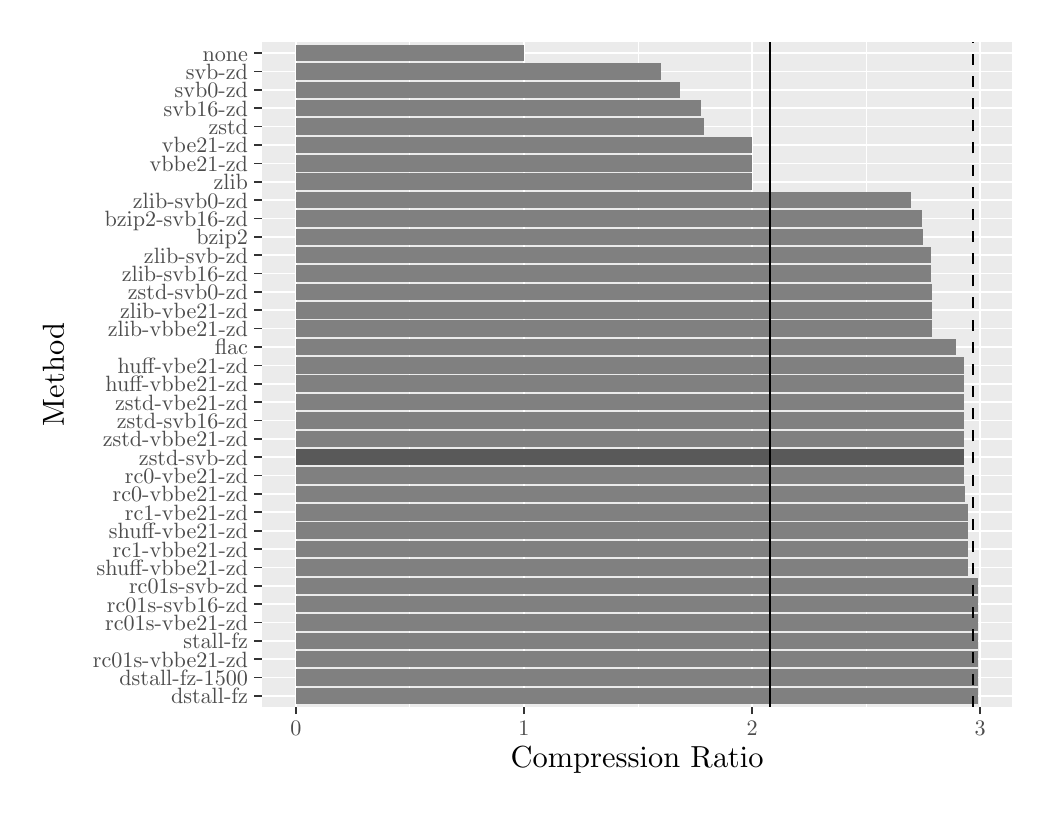
\begin{tikzpicture}[x=1pt,y=0.95pt]
\definecolor{fillColor}{RGB}{255,255,255}
\path[use as bounding box,fill=fillColor,fill opacity=0.00] (0,0) rectangle (361.35,289.08);
\begin{scope}
\path[clip] (  0.00,  0.00) rectangle (361.35,289.08);
\definecolor{drawColor}{RGB}{255,255,255}
\definecolor{fillColor}{RGB}{255,255,255}

\path[draw=drawColor,line width= 0.6pt,line join=round,line cap=round,fill=fillColor] (  0.00,  0.00) rectangle (361.35,289.08);
\end{scope}
\begin{scope}
\path[clip] ( 84.57, 30.69) rectangle (355.85,283.58);
\definecolor{fillColor}{gray}{0.92}

\path[fill=fillColor] ( 84.57, 30.69) rectangle (355.85,283.58);
\definecolor{drawColor}{RGB}{255,255,255}

\path[draw=drawColor,line width= 0.3pt,line join=round] (138.12, 30.69) --
	(138.12,283.58);

\path[draw=drawColor,line width= 0.3pt,line join=round] (220.55, 30.69) --
	(220.55,283.58);

\path[draw=drawColor,line width= 0.3pt,line join=round] (302.98, 30.69) --
	(302.98,283.58);

\path[draw=drawColor,line width= 0.6pt,line join=round] ( 84.57, 34.88) --
	(355.85, 34.88);

\path[draw=drawColor,line width= 0.6pt,line join=round] ( 84.57, 41.86) --
	(355.85, 41.86);

\path[draw=drawColor,line width= 0.6pt,line join=round] ( 84.57, 48.85) --
	(355.85, 48.85);

\path[draw=drawColor,line width= 0.6pt,line join=round] ( 84.57, 55.84) --
	(355.85, 55.84);

\path[draw=drawColor,line width= 0.6pt,line join=round] ( 84.57, 62.82) --
	(355.85, 62.82);

\path[draw=drawColor,line width= 0.6pt,line join=round] ( 84.57, 69.81) --
	(355.85, 69.81);

\path[draw=drawColor,line width= 0.6pt,line join=round] ( 84.57, 76.79) --
	(355.85, 76.79);

\path[draw=drawColor,line width= 0.6pt,line join=round] ( 84.57, 83.78) --
	(355.85, 83.78);

\path[draw=drawColor,line width= 0.6pt,line join=round] ( 84.57, 90.77) --
	(355.85, 90.77);

\path[draw=drawColor,line width= 0.6pt,line join=round] ( 84.57, 97.75) --
	(355.85, 97.75);

\path[draw=drawColor,line width= 0.6pt,line join=round] ( 84.57,104.74) --
	(355.85,104.74);

\path[draw=drawColor,line width= 0.6pt,line join=round] ( 84.57,111.72) --
	(355.85,111.72);

\path[draw=drawColor,line width= 0.6pt,line join=round] ( 84.57,118.71) --
	(355.85,118.71);

\path[draw=drawColor,line width= 0.6pt,line join=round] ( 84.57,125.70) --
	(355.85,125.70);

\path[draw=drawColor,line width= 0.6pt,line join=round] ( 84.57,132.68) --
	(355.85,132.68);

\path[draw=drawColor,line width= 0.6pt,line join=round] ( 84.57,139.67) --
	(355.85,139.67);

\path[draw=drawColor,line width= 0.6pt,line join=round] ( 84.57,146.65) --
	(355.85,146.65);

\path[draw=drawColor,line width= 0.6pt,line join=round] ( 84.57,153.64) --
	(355.85,153.64);

\path[draw=drawColor,line width= 0.6pt,line join=round] ( 84.57,160.63) --
	(355.85,160.63);

\path[draw=drawColor,line width= 0.6pt,line join=round] ( 84.57,167.61) --
	(355.85,167.61);

\path[draw=drawColor,line width= 0.6pt,line join=round] ( 84.57,174.60) --
	(355.85,174.60);

\path[draw=drawColor,line width= 0.6pt,line join=round] ( 84.57,181.58) --
	(355.85,181.58);

\path[draw=drawColor,line width= 0.6pt,line join=round] ( 84.57,188.57) --
	(355.85,188.57);

\path[draw=drawColor,line width= 0.6pt,line join=round] ( 84.57,195.56) --
	(355.85,195.56);

\path[draw=drawColor,line width= 0.6pt,line join=round] ( 84.57,202.54) --
	(355.85,202.54);

\path[draw=drawColor,line width= 0.6pt,line join=round] ( 84.57,209.53) --
	(355.85,209.53);

\path[draw=drawColor,line width= 0.6pt,line join=round] ( 84.57,216.51) --
	(355.85,216.51);

\path[draw=drawColor,line width= 0.6pt,line join=round] ( 84.57,223.50) --
	(355.85,223.50);

\path[draw=drawColor,line width= 0.6pt,line join=round] ( 84.57,230.49) --
	(355.85,230.49);

\path[draw=drawColor,line width= 0.6pt,line join=round] ( 84.57,237.47) --
	(355.85,237.47);

\path[draw=drawColor,line width= 0.6pt,line join=round] ( 84.57,244.46) --
	(355.85,244.46);

\path[draw=drawColor,line width= 0.6pt,line join=round] ( 84.57,251.44) --
	(355.85,251.44);

\path[draw=drawColor,line width= 0.6pt,line join=round] ( 84.57,258.43) --
	(355.85,258.43);

\path[draw=drawColor,line width= 0.6pt,line join=round] ( 84.57,265.42) --
	(355.85,265.42);

\path[draw=drawColor,line width= 0.6pt,line join=round] ( 84.57,272.40) --
	(355.85,272.40);

\path[draw=drawColor,line width= 0.6pt,line join=round] ( 84.57,279.39) --
	(355.85,279.39);

\path[draw=drawColor,line width= 0.6pt,line join=round] ( 96.90, 30.69) --
	( 96.90,283.58);

\path[draw=drawColor,line width= 0.6pt,line join=round] (179.34, 30.69) --
	(179.34,283.58);

\path[draw=drawColor,line width= 0.6pt,line join=round] (261.77, 30.69) --
	(261.77,283.58);

\path[draw=drawColor,line width= 0.6pt,line join=round] (344.20, 30.69) --
	(344.20,283.58);
\definecolor{fillColor}{gray}{0.50}

\path[fill=fillColor] ( 96.90,276.24) rectangle (179.34,282.53);

\path[fill=fillColor] ( 96.90,227.34) rectangle (261.89,233.63);

\path[fill=fillColor] ( 96.90,248.30) rectangle (244.53,254.59);

\path[fill=fillColor] ( 96.90,206.38) rectangle (323.60,212.67);

\path[fill=fillColor] ( 96.90,269.26) rectangle (228.79,275.55);

\path[fill=fillColor] ( 96.90,255.29) rectangle (243.44,261.57);

\path[fill=fillColor] ( 96.90,262.27) rectangle (235.60,268.56);

\path[fill=fillColor] ( 96.90,241.31) rectangle (261.73,247.60);

\path[fill=fillColor] ( 96.90,234.33) rectangle (261.75,240.62);
\definecolor{fillColor}{gray}{0.35}

\path[fill=fillColor] ( 96.90,122.55) rectangle (338.30,128.84);
\definecolor{fillColor}{gray}{0.50}

\path[fill=fillColor] ( 96.90,136.52) rectangle (338.29,142.81);

\path[fill=fillColor] ( 96.90,185.43) rectangle (326.87,191.71);

\path[fill=fillColor] ( 96.90,143.51) rectangle (338.27,149.80);

\path[fill=fillColor] ( 96.90,129.54) rectangle (338.30,135.83);

\path[fill=fillColor] ( 96.90,199.40) rectangle (326.35,205.69);

\path[fill=fillColor] ( 96.90,192.41) rectangle (326.57,198.70);

\path[fill=fillColor] ( 96.90,220.36) rectangle (319.24,226.64);

\path[fill=fillColor] ( 96.90,178.44) rectangle (326.91,184.73);

\path[fill=fillColor] ( 96.90,171.45) rectangle (326.93,177.74);

\path[fill=fillColor] ( 96.90,213.37) rectangle (322.98,219.66);

\path[fill=fillColor] ( 96.90,164.47) rectangle (335.41,170.76);

\path[fill=fillColor] ( 96.90,157.48) rectangle (338.21,163.77);

\path[fill=fillColor] ( 96.90, 94.61) rectangle (339.89,100.90);

\path[fill=fillColor] ( 96.90,115.57) rectangle (338.49,121.85);

\path[fill=fillColor] ( 96.90,101.59) rectangle (339.87,107.88);

\path[fill=fillColor] ( 96.90, 59.68) rectangle (343.45, 65.97);

\path[fill=fillColor] ( 96.90,150.50) rectangle (338.24,156.78);

\path[fill=fillColor] ( 96.90, 80.64) rectangle (339.93, 86.92);

\path[fill=fillColor] ( 96.90,108.58) rectangle (338.52,114.87);

\path[fill=fillColor] ( 96.90, 87.62) rectangle (339.90, 93.91);

\path[fill=fillColor] ( 96.90, 45.71) rectangle (343.48, 51.99);

\path[fill=fillColor] ( 96.90, 52.69) rectangle (343.47, 58.98);

\path[fill=fillColor] ( 96.90, 73.65) rectangle (343.42, 79.94);

\path[fill=fillColor] ( 96.90, 66.66) rectangle (343.42, 72.95);

\path[fill=fillColor] ( 96.90, 31.73) rectangle (343.52, 38.02);

\path[fill=fillColor] ( 96.90, 38.72) rectangle (343.52, 45.01);
\definecolor{drawColor}{RGB}{0,0,0}

\path[draw=drawColor,line width= 0.6pt,line join=round] (268.19, 30.69) -- (268.19,283.58);

\path[draw=drawColor,line width= 0.6pt,dash pattern=on 4pt off 4pt ,line join=round] (341.60, 30.69) -- (341.60,283.58);
\end{scope}
\begin{scope}
\path[clip] (  0.00,  0.00) rectangle (361.35,289.08);
\definecolor{drawColor}{gray}{0.30}

\node[text=drawColor,anchor=base east,inner sep=0pt, outer sep=0pt, scale=  0.80] at ( 79.62, 31.85) {dstall-fz};

\node[text=drawColor,anchor=base east,inner sep=0pt, outer sep=0pt, scale=  0.80] at ( 79.62, 38.83) {dstall-fz-1500};

\node[text=drawColor,anchor=base east,inner sep=0pt, outer sep=0pt, scale=  0.80] at ( 79.62, 45.82) {rc01s-vbbe21-zd};

\node[text=drawColor,anchor=base east,inner sep=0pt, outer sep=0pt, scale=  0.80] at ( 79.62, 52.81) {stall-fz};

\node[text=drawColor,anchor=base east,inner sep=0pt, outer sep=0pt, scale=  0.80] at ( 79.62, 59.79) {rc01s-vbe21-zd};

\node[text=drawColor,anchor=base east,inner sep=0pt, outer sep=0pt, scale=  0.80] at ( 79.62, 66.78) {rc01s-svb16-zd};

\node[text=drawColor,anchor=base east,inner sep=0pt, outer sep=0pt, scale=  0.80] at ( 79.62, 73.76) {rc01s-svb-zd};

\node[text=drawColor,anchor=base east,inner sep=0pt, outer sep=0pt, scale=  0.80] at ( 79.62, 80.75) {shuff-vbbe21-zd};

\node[text=drawColor,anchor=base east,inner sep=0pt, outer sep=0pt, scale=  0.80] at ( 79.62, 87.74) {rc1-vbbe21-zd};

\node[text=drawColor,anchor=base east,inner sep=0pt, outer sep=0pt, scale=  0.80] at ( 79.62, 94.72) {shuff-vbe21-zd};

\node[text=drawColor,anchor=base east,inner sep=0pt, outer sep=0pt, scale=  0.80] at ( 79.62,101.71) {rc1-vbe21-zd};

\node[text=drawColor,anchor=base east,inner sep=0pt, outer sep=0pt, scale=  0.80] at ( 79.62,108.69) {rc0-vbbe21-zd};

\node[text=drawColor,anchor=base east,inner sep=0pt, outer sep=0pt, scale=  0.80] at ( 79.62,115.68) {rc0-vbe21-zd};

\node[text=drawColor,anchor=base east,inner sep=0pt, outer sep=0pt, scale=  0.80] at ( 79.62,122.67) {zstd-svb-zd};

\node[text=drawColor,anchor=base east,inner sep=0pt, outer sep=0pt, scale=  0.80] at ( 79.62,129.65) {zstd-vbbe21-zd};

\node[text=drawColor,anchor=base east,inner sep=0pt, outer sep=0pt, scale=  0.80] at ( 79.62,136.64) {zstd-svb16-zd};

\node[text=drawColor,anchor=base east,inner sep=0pt, outer sep=0pt, scale=  0.80] at ( 79.62,143.62) {zstd-vbe21-zd};

\node[text=drawColor,anchor=base east,inner sep=0pt, outer sep=0pt, scale=  0.80] at ( 79.62,150.61) {huff-vbbe21-zd};

\node[text=drawColor,anchor=base east,inner sep=0pt, outer sep=0pt, scale=  0.80] at ( 79.62,157.60) {huff-vbe21-zd};

\node[text=drawColor,anchor=base east,inner sep=0pt, outer sep=0pt, scale=  0.80] at ( 79.62,164.58) {flac};

\node[text=drawColor,anchor=base east,inner sep=0pt, outer sep=0pt, scale=  0.80] at ( 79.62,171.57) {zlib-vbbe21-zd};

\node[text=drawColor,anchor=base east,inner sep=0pt, outer sep=0pt, scale=  0.80] at ( 79.62,178.55) {zlib-vbe21-zd};

\node[text=drawColor,anchor=base east,inner sep=0pt, outer sep=0pt, scale=  0.80] at ( 79.62,185.54) {zstd-svb0-zd};

\node[text=drawColor,anchor=base east,inner sep=0pt, outer sep=0pt, scale=  0.80] at ( 79.62,192.53) {zlib-svb16-zd};

\node[text=drawColor,anchor=base east,inner sep=0pt, outer sep=0pt, scale=  0.80] at ( 79.62,199.51) {zlib-svb-zd};

\node[text=drawColor,anchor=base east,inner sep=0pt, outer sep=0pt, scale=  0.80] at ( 79.62,206.50) {bzip2};

\node[text=drawColor,anchor=base east,inner sep=0pt, outer sep=0pt, scale=  0.80] at ( 79.62,213.48) {bzip2-svb16-zd};

\node[text=drawColor,anchor=base east,inner sep=0pt, outer sep=0pt, scale=  0.80] at ( 79.62,220.47) {zlib-svb0-zd};

\node[text=drawColor,anchor=base east,inner sep=0pt, outer sep=0pt, scale=  0.80] at ( 79.62,227.46) {zlib};

\node[text=drawColor,anchor=base east,inner sep=0pt, outer sep=0pt, scale=  0.80] at ( 79.62,234.44) {vbbe21-zd};

\node[text=drawColor,anchor=base east,inner sep=0pt, outer sep=0pt, scale=  0.80] at ( 79.62,241.43) {vbe21-zd};

\node[text=drawColor,anchor=base east,inner sep=0pt, outer sep=0pt, scale=  0.80] at ( 79.62,248.41) {zstd};

\node[text=drawColor,anchor=base east,inner sep=0pt, outer sep=0pt, scale=  0.80] at ( 79.62,255.40) {svb16-zd};

\node[text=drawColor,anchor=base east,inner sep=0pt, outer sep=0pt, scale=  0.80] at ( 79.62,262.39) {svb0-zd};

\node[text=drawColor,anchor=base east,inner sep=0pt, outer sep=0pt, scale=  0.80] at ( 79.62,269.37) {svb-zd};

\node[text=drawColor,anchor=base east,inner sep=0pt, outer sep=0pt, scale=  0.80] at ( 79.62,276.36) {none};
\end{scope}
\begin{scope}
\path[clip] (  0.00,  0.00) rectangle (361.35,289.08);
\definecolor{drawColor}{gray}{0.20}

\path[draw=drawColor,line width= 0.6pt,line join=round] ( 81.82, 34.88) --
	( 84.57, 34.88);

\path[draw=drawColor,line width= 0.6pt,line join=round] ( 81.82, 41.86) --
	( 84.57, 41.86);

\path[draw=drawColor,line width= 0.6pt,line join=round] ( 81.82, 48.85) --
	( 84.57, 48.85);

\path[draw=drawColor,line width= 0.6pt,line join=round] ( 81.82, 55.84) --
	( 84.57, 55.84);

\path[draw=drawColor,line width= 0.6pt,line join=round] ( 81.82, 62.82) --
	( 84.57, 62.82);

\path[draw=drawColor,line width= 0.6pt,line join=round] ( 81.82, 69.81) --
	( 84.57, 69.81);

\path[draw=drawColor,line width= 0.6pt,line join=round] ( 81.82, 76.79) --
	( 84.57, 76.79);

\path[draw=drawColor,line width= 0.6pt,line join=round] ( 81.82, 83.78) --
	( 84.57, 83.78);

\path[draw=drawColor,line width= 0.6pt,line join=round] ( 81.82, 90.77) --
	( 84.57, 90.77);

\path[draw=drawColor,line width= 0.6pt,line join=round] ( 81.82, 97.75) --
	( 84.57, 97.75);

\path[draw=drawColor,line width= 0.6pt,line join=round] ( 81.82,104.74) --
	( 84.57,104.74);

\path[draw=drawColor,line width= 0.6pt,line join=round] ( 81.82,111.72) --
	( 84.57,111.72);

\path[draw=drawColor,line width= 0.6pt,line join=round] ( 81.82,118.71) --
	( 84.57,118.71);

\path[draw=drawColor,line width= 0.6pt,line join=round] ( 81.82,125.70) --
	( 84.57,125.70);

\path[draw=drawColor,line width= 0.6pt,line join=round] ( 81.82,132.68) --
	( 84.57,132.68);

\path[draw=drawColor,line width= 0.6pt,line join=round] ( 81.82,139.67) --
	( 84.57,139.67);

\path[draw=drawColor,line width= 0.6pt,line join=round] ( 81.82,146.65) --
	( 84.57,146.65);

\path[draw=drawColor,line width= 0.6pt,line join=round] ( 81.82,153.64) --
	( 84.57,153.64);

\path[draw=drawColor,line width= 0.6pt,line join=round] ( 81.82,160.63) --
	( 84.57,160.63);

\path[draw=drawColor,line width= 0.6pt,line join=round] ( 81.82,167.61) --
	( 84.57,167.61);

\path[draw=drawColor,line width= 0.6pt,line join=round] ( 81.82,174.60) --
	( 84.57,174.60);

\path[draw=drawColor,line width= 0.6pt,line join=round] ( 81.82,181.58) --
	( 84.57,181.58);

\path[draw=drawColor,line width= 0.6pt,line join=round] ( 81.82,188.57) --
	( 84.57,188.57);

\path[draw=drawColor,line width= 0.6pt,line join=round] ( 81.82,195.56) --
	( 84.57,195.56);

\path[draw=drawColor,line width= 0.6pt,line join=round] ( 81.82,202.54) --
	( 84.57,202.54);

\path[draw=drawColor,line width= 0.6pt,line join=round] ( 81.82,209.53) --
	( 84.57,209.53);

\path[draw=drawColor,line width= 0.6pt,line join=round] ( 81.82,216.51) --
	( 84.57,216.51);

\path[draw=drawColor,line width= 0.6pt,line join=round] ( 81.82,223.50) --
	( 84.57,223.50);

\path[draw=drawColor,line width= 0.6pt,line join=round] ( 81.82,230.49) --
	( 84.57,230.49);

\path[draw=drawColor,line width= 0.6pt,line join=round] ( 81.82,237.47) --
	( 84.57,237.47);

\path[draw=drawColor,line width= 0.6pt,line join=round] ( 81.82,244.46) --
	( 84.57,244.46);

\path[draw=drawColor,line width= 0.6pt,line join=round] ( 81.82,251.44) --
	( 84.57,251.44);

\path[draw=drawColor,line width= 0.6pt,line join=round] ( 81.82,258.43) --
	( 84.57,258.43);

\path[draw=drawColor,line width= 0.6pt,line join=round] ( 81.82,265.42) --
	( 84.57,265.42);

\path[draw=drawColor,line width= 0.6pt,line join=round] ( 81.82,272.40) --
	( 84.57,272.40);

\path[draw=drawColor,line width= 0.6pt,line join=round] ( 81.82,279.39) --
	( 84.57,279.39);
\end{scope}
\begin{scope}
\path[clip] (  0.00,  0.00) rectangle (361.35,289.08);
\definecolor{drawColor}{gray}{0.20}

\path[draw=drawColor,line width= 0.6pt,line join=round] ( 96.90, 27.94) --
	( 96.90, 30.69);

\path[draw=drawColor,line width= 0.6pt,line join=round] (179.34, 27.94) --
	(179.34, 30.69);

\path[draw=drawColor,line width= 0.6pt,line join=round] (261.77, 27.94) --
	(261.77, 30.69);

\path[draw=drawColor,line width= 0.6pt,line join=round] (344.20, 27.94) --
	(344.20, 30.69);
\end{scope}
\begin{scope}
\path[clip] (  0.00,  0.00) rectangle (361.35,289.08);
\definecolor{drawColor}{gray}{0.30}

\node[text=drawColor,anchor=base,inner sep=0pt, outer sep=0pt, scale=  0.80] at ( 96.90, 19.68) {0};

\node[text=drawColor,anchor=base,inner sep=0pt, outer sep=0pt, scale=  0.80] at (179.34, 19.68) {1};

\node[text=drawColor,anchor=base,inner sep=0pt, outer sep=0pt, scale=  0.80] at (261.77, 19.68) {2};

\node[text=drawColor,anchor=base,inner sep=0pt, outer sep=0pt, scale=  0.80] at (344.20, 19.68) {3};
\end{scope}
\begin{scope}
\path[clip] (  0.00,  0.00) rectangle (361.35,289.08);
\definecolor{drawColor}{RGB}{0,0,0}

\node[text=drawColor,anchor=base,inner sep=0pt, outer sep=0pt, scale=  1.10] at (220.21,  7.64) {Compression Ratio};
\end{scope}
\begin{scope}
\path[clip] (  0.00,  0.00) rectangle (361.35,289.08);
\definecolor{drawColor}{RGB}{0,0,0}

\node[text=drawColor,rotate= 90.00,anchor=base,inner sep=0pt, outer sep=0pt, scale=  1.10] at ( 13.08,157.13) {Method};
\end{scope}
\end{tikzpicture}

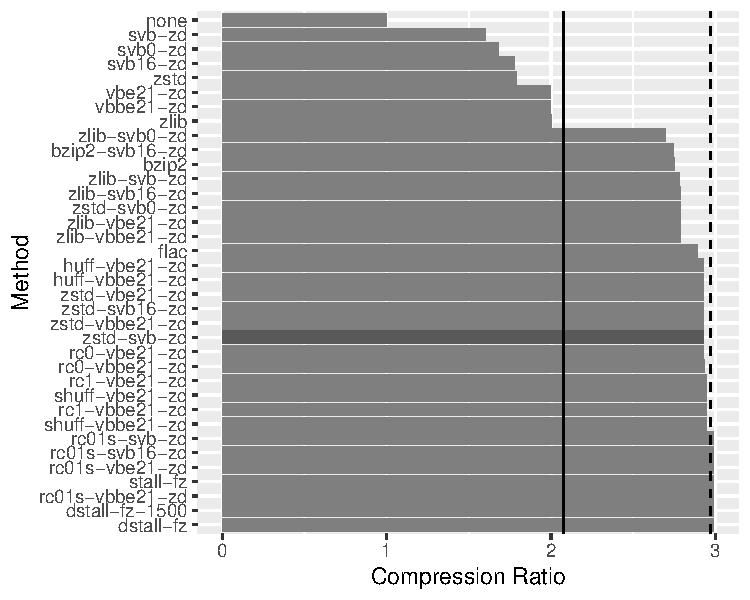
\includegraphics[scale=0.9]{plots/reads.blow5.test.ratio.bar.pdf}
	\caption[The compression ratio of each method on the
	data.]{\label{fig:results-ratio}The compression ratio of each method on the
	data. The state-of-the-art method is highlighted in a darker grey.
	The solid and dotted vertical lines represents the compression ratio
	equivalent of the entropy of the data and its deltas respectively.}
\end{figure}

\begin{figure}
\centering
%% Created by tikzDevice version 0.12.3.1 on 2022-11-04 11:04:58
% !TEX encoding = UTF-8 Unicode
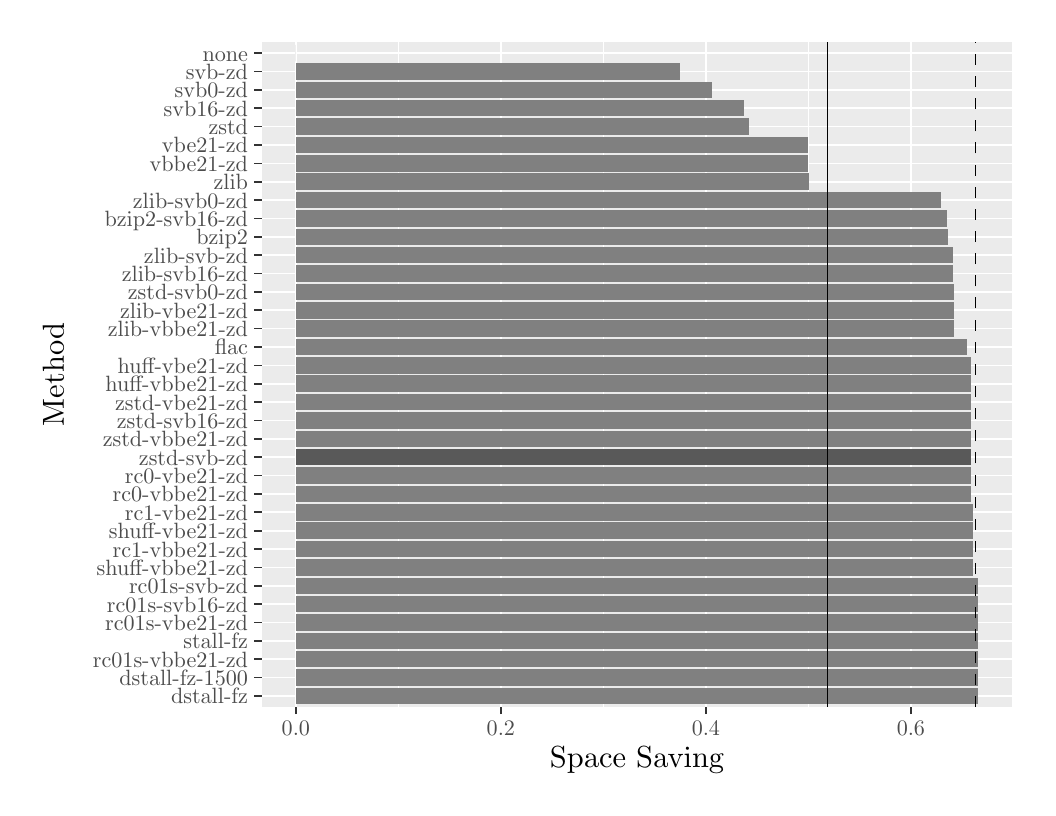
\begin{tikzpicture}[x=1pt,y=0.95pt]
\definecolor{fillColor}{RGB}{255,255,255}
\path[use as bounding box,fill=fillColor,fill opacity=0.00] (0,0) rectangle (361.35,289.08);
\begin{scope}
\path[clip] (  0.00,  0.00) rectangle (361.35,289.08);
\definecolor{drawColor}{RGB}{255,255,255}
\definecolor{fillColor}{RGB}{255,255,255}

\path[draw=drawColor,line width= 0.6pt,line join=round,line cap=round,fill=fillColor] (  0.00,  0.00) rectangle (361.35,289.08);
\end{scope}
\begin{scope}
\path[clip] ( 84.57, 30.69) rectangle (355.85,283.58);
\definecolor{fillColor}{gray}{0.92}

\path[fill=fillColor] ( 84.57, 30.69) rectangle (355.85,283.58);
\definecolor{drawColor}{RGB}{255,255,255}

\path[draw=drawColor,line width= 0.3pt,line join=round] (133.95, 30.69) --
	(133.95,283.58);

\path[draw=drawColor,line width= 0.3pt,line join=round] (208.03, 30.69) --
	(208.03,283.58);

\path[draw=drawColor,line width= 0.3pt,line join=round] (282.12, 30.69) --
	(282.12,283.58);

\path[draw=drawColor,line width= 0.6pt,line join=round] ( 84.57, 34.88) --
	(355.85, 34.88);

\path[draw=drawColor,line width= 0.6pt,line join=round] ( 84.57, 41.86) --
	(355.85, 41.86);

\path[draw=drawColor,line width= 0.6pt,line join=round] ( 84.57, 48.85) --
	(355.85, 48.85);

\path[draw=drawColor,line width= 0.6pt,line join=round] ( 84.57, 55.84) --
	(355.85, 55.84);

\path[draw=drawColor,line width= 0.6pt,line join=round] ( 84.57, 62.82) --
	(355.85, 62.82);

\path[draw=drawColor,line width= 0.6pt,line join=round] ( 84.57, 69.81) --
	(355.85, 69.81);

\path[draw=drawColor,line width= 0.6pt,line join=round] ( 84.57, 76.79) --
	(355.85, 76.79);

\path[draw=drawColor,line width= 0.6pt,line join=round] ( 84.57, 83.78) --
	(355.85, 83.78);

\path[draw=drawColor,line width= 0.6pt,line join=round] ( 84.57, 90.77) --
	(355.85, 90.77);

\path[draw=drawColor,line width= 0.6pt,line join=round] ( 84.57, 97.75) --
	(355.85, 97.75);

\path[draw=drawColor,line width= 0.6pt,line join=round] ( 84.57,104.74) --
	(355.85,104.74);

\path[draw=drawColor,line width= 0.6pt,line join=round] ( 84.57,111.72) --
	(355.85,111.72);

\path[draw=drawColor,line width= 0.6pt,line join=round] ( 84.57,118.71) --
	(355.85,118.71);

\path[draw=drawColor,line width= 0.6pt,line join=round] ( 84.57,125.70) --
	(355.85,125.70);

\path[draw=drawColor,line width= 0.6pt,line join=round] ( 84.57,132.68) --
	(355.85,132.68);

\path[draw=drawColor,line width= 0.6pt,line join=round] ( 84.57,139.67) --
	(355.85,139.67);

\path[draw=drawColor,line width= 0.6pt,line join=round] ( 84.57,146.65) --
	(355.85,146.65);

\path[draw=drawColor,line width= 0.6pt,line join=round] ( 84.57,153.64) --
	(355.85,153.64);

\path[draw=drawColor,line width= 0.6pt,line join=round] ( 84.57,160.63) --
	(355.85,160.63);

\path[draw=drawColor,line width= 0.6pt,line join=round] ( 84.57,167.61) --
	(355.85,167.61);

\path[draw=drawColor,line width= 0.6pt,line join=round] ( 84.57,174.60) --
	(355.85,174.60);

\path[draw=drawColor,line width= 0.6pt,line join=round] ( 84.57,181.58) --
	(355.85,181.58);

\path[draw=drawColor,line width= 0.6pt,line join=round] ( 84.57,188.57) --
	(355.85,188.57);

\path[draw=drawColor,line width= 0.6pt,line join=round] ( 84.57,195.56) --
	(355.85,195.56);

\path[draw=drawColor,line width= 0.6pt,line join=round] ( 84.57,202.54) --
	(355.85,202.54);

\path[draw=drawColor,line width= 0.6pt,line join=round] ( 84.57,209.53) --
	(355.85,209.53);

\path[draw=drawColor,line width= 0.6pt,line join=round] ( 84.57,216.51) --
	(355.85,216.51);

\path[draw=drawColor,line width= 0.6pt,line join=round] ( 84.57,223.50) --
	(355.85,223.50);

\path[draw=drawColor,line width= 0.6pt,line join=round] ( 84.57,230.49) --
	(355.85,230.49);

\path[draw=drawColor,line width= 0.6pt,line join=round] ( 84.57,237.47) --
	(355.85,237.47);

\path[draw=drawColor,line width= 0.6pt,line join=round] ( 84.57,244.46) --
	(355.85,244.46);

\path[draw=drawColor,line width= 0.6pt,line join=round] ( 84.57,251.44) --
	(355.85,251.44);

\path[draw=drawColor,line width= 0.6pt,line join=round] ( 84.57,258.43) --
	(355.85,258.43);

\path[draw=drawColor,line width= 0.6pt,line join=round] ( 84.57,265.42) --
	(355.85,265.42);

\path[draw=drawColor,line width= 0.6pt,line join=round] ( 84.57,272.40) --
	(355.85,272.40);

\path[draw=drawColor,line width= 0.6pt,line join=round] ( 84.57,279.39) --
	(355.85,279.39);

\path[draw=drawColor,line width= 0.6pt,line join=round] ( 96.90, 30.69) --
	( 96.90,283.58);

\path[draw=drawColor,line width= 0.6pt,line join=round] (170.99, 30.69) --
	(170.99,283.58);

\path[draw=drawColor,line width= 0.6pt,line join=round] (245.08, 30.69) --
	(245.08,283.58);

\path[draw=drawColor,line width= 0.6pt,line join=round] (319.16, 30.69) --
	(319.16,283.58);
\definecolor{fillColor}{gray}{0.50}

\path[fill=fillColor] ( 96.90,276.24) rectangle ( 96.90,282.53);

\path[fill=fillColor] ( 96.90,227.34) rectangle (282.26,233.63);

\path[fill=fillColor] ( 96.90,248.30) rectangle (260.50,254.59);

\path[fill=fillColor] ( 96.90,206.38) rectangle (332.64,212.67);

\path[fill=fillColor] ( 96.90,269.26) rectangle (235.81,275.55);

\path[fill=fillColor] ( 96.90,255.29) rectangle (258.96,261.57);

\path[fill=fillColor] ( 96.90,262.27) rectangle (247.18,268.56);

\path[fill=fillColor] ( 96.90,241.31) rectangle (282.08,247.60);

\path[fill=fillColor] ( 96.90,234.33) rectangle (282.09,240.62);
\definecolor{fillColor}{gray}{0.35}

\path[fill=fillColor] ( 96.90,122.55) rectangle (340.84,128.84);
\definecolor{fillColor}{gray}{0.50}

\path[fill=fillColor] ( 96.90,136.52) rectangle (340.84,142.81);

\path[fill=fillColor] ( 96.90,185.43) rectangle (334.56,191.71);

\path[fill=fillColor] ( 96.90,143.51) rectangle (340.83,149.80);

\path[fill=fillColor] ( 96.90,129.54) rectangle (340.84,135.83);

\path[fill=fillColor] ( 96.90,199.40) rectangle (334.26,205.69);

\path[fill=fillColor] ( 96.90,192.41) rectangle (334.38,198.70);

\path[fill=fillColor] ( 96.90,220.36) rectangle (330.00,226.64);

\path[fill=fillColor] ( 96.90,178.44) rectangle (334.58,184.73);

\path[fill=fillColor] ( 96.90,171.45) rectangle (334.59,177.74);

\path[fill=fillColor] ( 96.90,213.37) rectangle (332.27,219.66);

\path[fill=fillColor] ( 96.90,164.47) rectangle (339.31,170.76);

\path[fill=fillColor] ( 96.90,157.48) rectangle (340.79,163.77);

\path[fill=fillColor] ( 96.90, 94.61) rectangle (341.67,100.90);

\path[fill=fillColor] ( 96.90,115.57) rectangle (340.94,121.85);

\path[fill=fillColor] ( 96.90,101.59) rectangle (341.66,107.88);

\path[fill=fillColor] ( 96.90, 59.68) rectangle (343.48, 65.97);

\path[fill=fillColor] ( 96.90,150.50) rectangle (340.81,156.78);

\path[fill=fillColor] ( 96.90, 80.64) rectangle (341.69, 86.92);

\path[fill=fillColor] ( 96.90,108.58) rectangle (340.96,114.87);

\path[fill=fillColor] ( 96.90, 87.62) rectangle (341.68, 93.91);

\path[fill=fillColor] ( 96.90, 45.71) rectangle (343.50, 51.99);

\path[fill=fillColor] ( 96.90, 52.69) rectangle (343.49, 58.98);

\path[fill=fillColor] ( 96.90, 73.65) rectangle (343.47, 79.94);

\path[fill=fillColor] ( 96.90, 66.66) rectangle (343.47, 72.95);

\path[fill=fillColor] ( 96.90, 31.73) rectangle (343.52, 38.02);

\path[fill=fillColor] ( 96.90, 38.72) rectangle (343.52, 45.01);
\definecolor{drawColor}{RGB}{0,0,0}

\path[draw=drawColor,line width= 0.6pt,line join=round] (289.07, 30.69) -- (289.07,283.58);

\path[draw=drawColor,line width= 0.6pt,dash pattern=on 4pt off 4pt ,line join=round] (342.55, 30.69) -- (342.55,283.58);
\end{scope}
\begin{scope}
\path[clip] (  0.00,  0.00) rectangle (361.35,289.08);
\definecolor{drawColor}{gray}{0.30}

\node[text=drawColor,anchor=base east,inner sep=0pt, outer sep=0pt, scale=  0.80] at ( 79.62, 31.85) {dstall-fz};

\node[text=drawColor,anchor=base east,inner sep=0pt, outer sep=0pt, scale=  0.80] at ( 79.62, 38.83) {dstall-fz-1500};

\node[text=drawColor,anchor=base east,inner sep=0pt, outer sep=0pt, scale=  0.80] at ( 79.62, 45.82) {rc01s-vbbe21-zd};

\node[text=drawColor,anchor=base east,inner sep=0pt, outer sep=0pt, scale=  0.80] at ( 79.62, 52.81) {stall-fz};

\node[text=drawColor,anchor=base east,inner sep=0pt, outer sep=0pt, scale=  0.80] at ( 79.62, 59.79) {rc01s-vbe21-zd};

\node[text=drawColor,anchor=base east,inner sep=0pt, outer sep=0pt, scale=  0.80] at ( 79.62, 66.78) {rc01s-svb16-zd};

\node[text=drawColor,anchor=base east,inner sep=0pt, outer sep=0pt, scale=  0.80] at ( 79.62, 73.76) {rc01s-svb-zd};

\node[text=drawColor,anchor=base east,inner sep=0pt, outer sep=0pt, scale=  0.80] at ( 79.62, 80.75) {shuff-vbbe21-zd};

\node[text=drawColor,anchor=base east,inner sep=0pt, outer sep=0pt, scale=  0.80] at ( 79.62, 87.74) {rc1-vbbe21-zd};

\node[text=drawColor,anchor=base east,inner sep=0pt, outer sep=0pt, scale=  0.80] at ( 79.62, 94.72) {shuff-vbe21-zd};

\node[text=drawColor,anchor=base east,inner sep=0pt, outer sep=0pt, scale=  0.80] at ( 79.62,101.71) {rc1-vbe21-zd};

\node[text=drawColor,anchor=base east,inner sep=0pt, outer sep=0pt, scale=  0.80] at ( 79.62,108.69) {rc0-vbbe21-zd};

\node[text=drawColor,anchor=base east,inner sep=0pt, outer sep=0pt, scale=  0.80] at ( 79.62,115.68) {rc0-vbe21-zd};

\node[text=drawColor,anchor=base east,inner sep=0pt, outer sep=0pt, scale=  0.80] at ( 79.62,122.67) {zstd-svb-zd};

\node[text=drawColor,anchor=base east,inner sep=0pt, outer sep=0pt, scale=  0.80] at ( 79.62,129.65) {zstd-vbbe21-zd};

\node[text=drawColor,anchor=base east,inner sep=0pt, outer sep=0pt, scale=  0.80] at ( 79.62,136.64) {zstd-svb16-zd};

\node[text=drawColor,anchor=base east,inner sep=0pt, outer sep=0pt, scale=  0.80] at ( 79.62,143.62) {zstd-vbe21-zd};

\node[text=drawColor,anchor=base east,inner sep=0pt, outer sep=0pt, scale=  0.80] at ( 79.62,150.61) {huff-vbbe21-zd};

\node[text=drawColor,anchor=base east,inner sep=0pt, outer sep=0pt, scale=  0.80] at ( 79.62,157.60) {huff-vbe21-zd};

\node[text=drawColor,anchor=base east,inner sep=0pt, outer sep=0pt, scale=  0.80] at ( 79.62,164.58) {flac};

\node[text=drawColor,anchor=base east,inner sep=0pt, outer sep=0pt, scale=  0.80] at ( 79.62,171.57) {zlib-vbbe21-zd};

\node[text=drawColor,anchor=base east,inner sep=0pt, outer sep=0pt, scale=  0.80] at ( 79.62,178.55) {zlib-vbe21-zd};

\node[text=drawColor,anchor=base east,inner sep=0pt, outer sep=0pt, scale=  0.80] at ( 79.62,185.54) {zstd-svb0-zd};

\node[text=drawColor,anchor=base east,inner sep=0pt, outer sep=0pt, scale=  0.80] at ( 79.62,192.53) {zlib-svb16-zd};

\node[text=drawColor,anchor=base east,inner sep=0pt, outer sep=0pt, scale=  0.80] at ( 79.62,199.51) {zlib-svb-zd};

\node[text=drawColor,anchor=base east,inner sep=0pt, outer sep=0pt, scale=  0.80] at ( 79.62,206.50) {bzip2};

\node[text=drawColor,anchor=base east,inner sep=0pt, outer sep=0pt, scale=  0.80] at ( 79.62,213.48) {bzip2-svb16-zd};

\node[text=drawColor,anchor=base east,inner sep=0pt, outer sep=0pt, scale=  0.80] at ( 79.62,220.47) {zlib-svb0-zd};

\node[text=drawColor,anchor=base east,inner sep=0pt, outer sep=0pt, scale=  0.80] at ( 79.62,227.46) {zlib};

\node[text=drawColor,anchor=base east,inner sep=0pt, outer sep=0pt, scale=  0.80] at ( 79.62,234.44) {vbbe21-zd};

\node[text=drawColor,anchor=base east,inner sep=0pt, outer sep=0pt, scale=  0.80] at ( 79.62,241.43) {vbe21-zd};

\node[text=drawColor,anchor=base east,inner sep=0pt, outer sep=0pt, scale=  0.80] at ( 79.62,248.41) {zstd};

\node[text=drawColor,anchor=base east,inner sep=0pt, outer sep=0pt, scale=  0.80] at ( 79.62,255.40) {svb16-zd};

\node[text=drawColor,anchor=base east,inner sep=0pt, outer sep=0pt, scale=  0.80] at ( 79.62,262.39) {svb0-zd};

\node[text=drawColor,anchor=base east,inner sep=0pt, outer sep=0pt, scale=  0.80] at ( 79.62,269.37) {svb-zd};

\node[text=drawColor,anchor=base east,inner sep=0pt, outer sep=0pt, scale=  0.80] at ( 79.62,276.36) {none};
\end{scope}
\begin{scope}
\path[clip] (  0.00,  0.00) rectangle (361.35,289.08);
\definecolor{drawColor}{gray}{0.20}

\path[draw=drawColor,line width= 0.6pt,line join=round] ( 81.82, 34.88) --
	( 84.57, 34.88);

\path[draw=drawColor,line width= 0.6pt,line join=round] ( 81.82, 41.86) --
	( 84.57, 41.86);

\path[draw=drawColor,line width= 0.6pt,line join=round] ( 81.82, 48.85) --
	( 84.57, 48.85);

\path[draw=drawColor,line width= 0.6pt,line join=round] ( 81.82, 55.84) --
	( 84.57, 55.84);

\path[draw=drawColor,line width= 0.6pt,line join=round] ( 81.82, 62.82) --
	( 84.57, 62.82);

\path[draw=drawColor,line width= 0.6pt,line join=round] ( 81.82, 69.81) --
	( 84.57, 69.81);

\path[draw=drawColor,line width= 0.6pt,line join=round] ( 81.82, 76.79) --
	( 84.57, 76.79);

\path[draw=drawColor,line width= 0.6pt,line join=round] ( 81.82, 83.78) --
	( 84.57, 83.78);

\path[draw=drawColor,line width= 0.6pt,line join=round] ( 81.82, 90.77) --
	( 84.57, 90.77);

\path[draw=drawColor,line width= 0.6pt,line join=round] ( 81.82, 97.75) --
	( 84.57, 97.75);

\path[draw=drawColor,line width= 0.6pt,line join=round] ( 81.82,104.74) --
	( 84.57,104.74);

\path[draw=drawColor,line width= 0.6pt,line join=round] ( 81.82,111.72) --
	( 84.57,111.72);

\path[draw=drawColor,line width= 0.6pt,line join=round] ( 81.82,118.71) --
	( 84.57,118.71);

\path[draw=drawColor,line width= 0.6pt,line join=round] ( 81.82,125.70) --
	( 84.57,125.70);

\path[draw=drawColor,line width= 0.6pt,line join=round] ( 81.82,132.68) --
	( 84.57,132.68);

\path[draw=drawColor,line width= 0.6pt,line join=round] ( 81.82,139.67) --
	( 84.57,139.67);

\path[draw=drawColor,line width= 0.6pt,line join=round] ( 81.82,146.65) --
	( 84.57,146.65);

\path[draw=drawColor,line width= 0.6pt,line join=round] ( 81.82,153.64) --
	( 84.57,153.64);

\path[draw=drawColor,line width= 0.6pt,line join=round] ( 81.82,160.63) --
	( 84.57,160.63);

\path[draw=drawColor,line width= 0.6pt,line join=round] ( 81.82,167.61) --
	( 84.57,167.61);

\path[draw=drawColor,line width= 0.6pt,line join=round] ( 81.82,174.60) --
	( 84.57,174.60);

\path[draw=drawColor,line width= 0.6pt,line join=round] ( 81.82,181.58) --
	( 84.57,181.58);

\path[draw=drawColor,line width= 0.6pt,line join=round] ( 81.82,188.57) --
	( 84.57,188.57);

\path[draw=drawColor,line width= 0.6pt,line join=round] ( 81.82,195.56) --
	( 84.57,195.56);

\path[draw=drawColor,line width= 0.6pt,line join=round] ( 81.82,202.54) --
	( 84.57,202.54);

\path[draw=drawColor,line width= 0.6pt,line join=round] ( 81.82,209.53) --
	( 84.57,209.53);

\path[draw=drawColor,line width= 0.6pt,line join=round] ( 81.82,216.51) --
	( 84.57,216.51);

\path[draw=drawColor,line width= 0.6pt,line join=round] ( 81.82,223.50) --
	( 84.57,223.50);

\path[draw=drawColor,line width= 0.6pt,line join=round] ( 81.82,230.49) --
	( 84.57,230.49);

\path[draw=drawColor,line width= 0.6pt,line join=round] ( 81.82,237.47) --
	( 84.57,237.47);

\path[draw=drawColor,line width= 0.6pt,line join=round] ( 81.82,244.46) --
	( 84.57,244.46);

\path[draw=drawColor,line width= 0.6pt,line join=round] ( 81.82,251.44) --
	( 84.57,251.44);

\path[draw=drawColor,line width= 0.6pt,line join=round] ( 81.82,258.43) --
	( 84.57,258.43);

\path[draw=drawColor,line width= 0.6pt,line join=round] ( 81.82,265.42) --
	( 84.57,265.42);

\path[draw=drawColor,line width= 0.6pt,line join=round] ( 81.82,272.40) --
	( 84.57,272.40);

\path[draw=drawColor,line width= 0.6pt,line join=round] ( 81.82,279.39) --
	( 84.57,279.39);
\end{scope}
\begin{scope}
\path[clip] (  0.00,  0.00) rectangle (361.35,289.08);
\definecolor{drawColor}{gray}{0.20}

\path[draw=drawColor,line width= 0.6pt,line join=round] ( 96.90, 27.94) --
	( 96.90, 30.69);

\path[draw=drawColor,line width= 0.6pt,line join=round] (170.99, 27.94) --
	(170.99, 30.69);

\path[draw=drawColor,line width= 0.6pt,line join=round] (245.08, 27.94) --
	(245.08, 30.69);

\path[draw=drawColor,line width= 0.6pt,line join=round] (319.16, 27.94) --
	(319.16, 30.69);
\end{scope}
\begin{scope}
\path[clip] (  0.00,  0.00) rectangle (361.35,289.08);
\definecolor{drawColor}{gray}{0.30}

\node[text=drawColor,anchor=base,inner sep=0pt, outer sep=0pt, scale=  0.80] at ( 96.90, 19.68) {0.0};

\node[text=drawColor,anchor=base,inner sep=0pt, outer sep=0pt, scale=  0.80] at (170.99, 19.68) {0.2};

\node[text=drawColor,anchor=base,inner sep=0pt, outer sep=0pt, scale=  0.80] at (245.08, 19.68) {0.4};

\node[text=drawColor,anchor=base,inner sep=0pt, outer sep=0pt, scale=  0.80] at (319.16, 19.68) {0.6};
\end{scope}
\begin{scope}
\path[clip] (  0.00,  0.00) rectangle (361.35,289.08);
\definecolor{drawColor}{RGB}{0,0,0}

\node[text=drawColor,anchor=base,inner sep=0pt, outer sep=0pt, scale=  1.10] at (220.21,  7.64) {Space Saving};
\end{scope}
\begin{scope}
\path[clip] (  0.00,  0.00) rectangle (361.35,289.08);
\definecolor{drawColor}{RGB}{0,0,0}

\node[text=drawColor,rotate= 90.00,anchor=base,inner sep=0pt, outer sep=0pt, scale=  1.10] at ( 13.08,157.13) {Method};
\end{scope}
\end{tikzpicture}

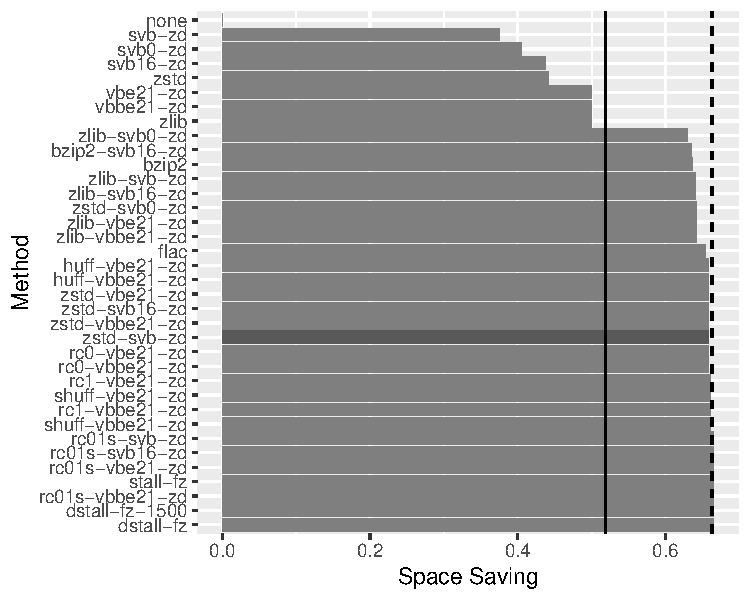
\includegraphics[scale=0.9]{plots/reads.blow5.test.ss.bar.pdf}
\caption{\label{fig:results-ss}The space saving of each method on the
	data. The state-of-the-art method is highlighted in a darker grey.
	The solid and dotted vertical lines represents the space saving
	equivalent of the entropy of the data and its deltas respectively.}
\end{figure}

\begin{figure}
\centering
%% Created by tikzDevice version 0.12.3.1 on 2022-11-04 11:24:38
% !TEX encoding = UTF-8 Unicode
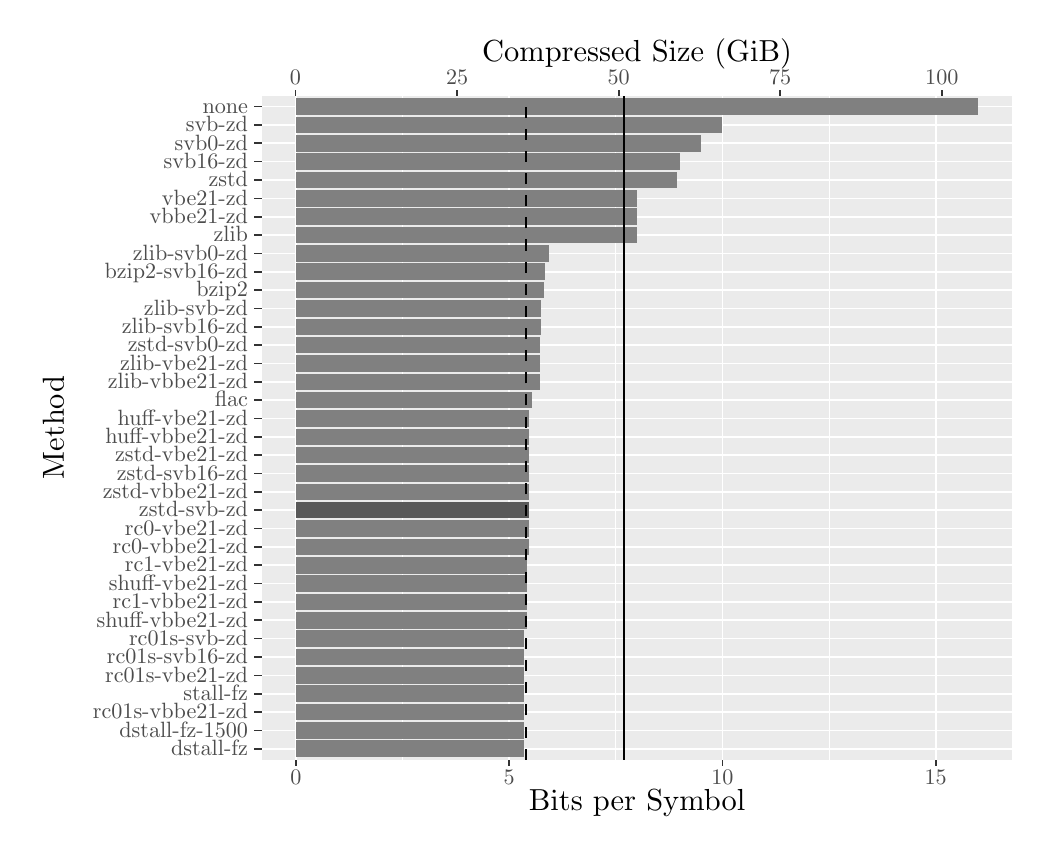
\begin{tikzpicture}[x=1pt,y=0.80pt]
\definecolor{fillColor}{RGB}{255,255,255}
\path[use as bounding box,fill=fillColor,fill opacity=0.00] (0,0) rectangle (361.35,361.35);
\begin{scope}
\path[clip] (  0.00,  0.00) rectangle (361.35,361.35);
\definecolor{drawColor}{RGB}{255,255,255}
\definecolor{fillColor}{RGB}{255,255,255}

\path[draw=drawColor,line width= 0.6pt,line join=round,line cap=round,fill=fillColor] (  0.00,  0.00) rectangle (361.35,361.35);
\end{scope}
\begin{scope}
\path[clip] ( 84.57, 30.69) rectangle (355.85,330.66);
\definecolor{fillColor}{gray}{0.92}

\path[fill=fillColor] ( 84.57, 30.69) rectangle (355.85,330.66);
\definecolor{drawColor}{RGB}{255,255,255}

\path[draw=drawColor,line width= 0.3pt,line join=round] (135.44, 30.69) --
	(135.44,330.66);

\path[draw=drawColor,line width= 0.3pt,line join=round] (212.50, 30.69) --
	(212.50,330.66);

\path[draw=drawColor,line width= 0.3pt,line join=round] (289.57, 30.69) --
	(289.57,330.66);

\path[draw=drawColor,line width= 0.6pt,line join=round] ( 84.57, 35.66) --
	(355.85, 35.66);

\path[draw=drawColor,line width= 0.6pt,line join=round] ( 84.57, 43.94) --
	(355.85, 43.94);

\path[draw=drawColor,line width= 0.6pt,line join=round] ( 84.57, 52.23) --
	(355.85, 52.23);

\path[draw=drawColor,line width= 0.6pt,line join=round] ( 84.57, 60.52) --
	(355.85, 60.52);

\path[draw=drawColor,line width= 0.6pt,line join=round] ( 84.57, 68.80) --
	(355.85, 68.80);

\path[draw=drawColor,line width= 0.6pt,line join=round] ( 84.57, 77.09) --
	(355.85, 77.09);

\path[draw=drawColor,line width= 0.6pt,line join=round] ( 84.57, 85.38) --
	(355.85, 85.38);

\path[draw=drawColor,line width= 0.6pt,line join=round] ( 84.57, 93.66) --
	(355.85, 93.66);

\path[draw=drawColor,line width= 0.6pt,line join=round] ( 84.57,101.95) --
	(355.85,101.95);

\path[draw=drawColor,line width= 0.6pt,line join=round] ( 84.57,110.24) --
	(355.85,110.24);

\path[draw=drawColor,line width= 0.6pt,line join=round] ( 84.57,118.52) --
	(355.85,118.52);

\path[draw=drawColor,line width= 0.6pt,line join=round] ( 84.57,126.81) --
	(355.85,126.81);

\path[draw=drawColor,line width= 0.6pt,line join=round] ( 84.57,135.10) --
	(355.85,135.10);

\path[draw=drawColor,line width= 0.6pt,line join=round] ( 84.57,143.38) --
	(355.85,143.38);

\path[draw=drawColor,line width= 0.6pt,line join=round] ( 84.57,151.67) --
	(355.85,151.67);

\path[draw=drawColor,line width= 0.6pt,line join=round] ( 84.57,159.96) --
	(355.85,159.96);

\path[draw=drawColor,line width= 0.6pt,line join=round] ( 84.57,168.24) --
	(355.85,168.24);

\path[draw=drawColor,line width= 0.6pt,line join=round] ( 84.57,176.53) --
	(355.85,176.53);

\path[draw=drawColor,line width= 0.6pt,line join=round] ( 84.57,184.82) --
	(355.85,184.82);

\path[draw=drawColor,line width= 0.6pt,line join=round] ( 84.57,193.11) --
	(355.85,193.11);

\path[draw=drawColor,line width= 0.6pt,line join=round] ( 84.57,201.39) --
	(355.85,201.39);

\path[draw=drawColor,line width= 0.6pt,line join=round] ( 84.57,209.68) --
	(355.85,209.68);

\path[draw=drawColor,line width= 0.6pt,line join=round] ( 84.57,217.97) --
	(355.85,217.97);

\path[draw=drawColor,line width= 0.6pt,line join=round] ( 84.57,226.25) --
	(355.85,226.25);

\path[draw=drawColor,line width= 0.6pt,line join=round] ( 84.57,234.54) --
	(355.85,234.54);

\path[draw=drawColor,line width= 0.6pt,line join=round] ( 84.57,242.83) --
	(355.85,242.83);

\path[draw=drawColor,line width= 0.6pt,line join=round] ( 84.57,251.11) --
	(355.85,251.11);

\path[draw=drawColor,line width= 0.6pt,line join=round] ( 84.57,259.40) --
	(355.85,259.40);

\path[draw=drawColor,line width= 0.6pt,line join=round] ( 84.57,267.69) --
	(355.85,267.69);

\path[draw=drawColor,line width= 0.6pt,line join=round] ( 84.57,275.97) --
	(355.85,275.97);

\path[draw=drawColor,line width= 0.6pt,line join=round] ( 84.57,284.26) --
	(355.85,284.26);

\path[draw=drawColor,line width= 0.6pt,line join=round] ( 84.57,292.55) --
	(355.85,292.55);

\path[draw=drawColor,line width= 0.6pt,line join=round] ( 84.57,300.83) --
	(355.85,300.83);

\path[draw=drawColor,line width= 0.6pt,line join=round] ( 84.57,309.12) --
	(355.85,309.12);

\path[draw=drawColor,line width= 0.6pt,line join=round] ( 84.57,317.41) --
	(355.85,317.41);

\path[draw=drawColor,line width= 0.6pt,line join=round] ( 84.57,325.69) --
	(355.85,325.69);

\path[draw=drawColor,line width= 0.6pt,line join=round] ( 96.90, 30.69) --
	( 96.90,330.66);

\path[draw=drawColor,line width= 0.6pt,line join=round] (173.97, 30.69) --
	(173.97,330.66);

\path[draw=drawColor,line width= 0.6pt,line join=round] (251.04, 30.69) --
	(251.04,330.66);

\path[draw=drawColor,line width= 0.6pt,line join=round] (328.10, 30.69) --
	(328.10,330.66);
\definecolor{fillColor}{gray}{0.50}

\path[fill=fillColor] ( 96.90,321.96) rectangle (343.52,329.42);

\path[fill=fillColor] ( 96.90,263.96) rectangle (220.12,271.41);

\path[fill=fillColor] ( 96.90,288.82) rectangle (234.61,296.27);

\path[fill=fillColor] ( 96.90,239.10) rectangle (186.58,246.55);

\path[fill=fillColor] ( 96.90,313.68) rectangle (251.05,321.13);

\path[fill=fillColor] ( 96.90,297.10) rectangle (235.63,304.56);

\path[fill=fillColor] ( 96.90,305.39) rectangle (243.48,312.85);

\path[fill=fillColor] ( 96.90,280.53) rectangle (220.24,287.99);

\path[fill=fillColor] ( 96.90,272.24) rectangle (220.23,279.70);
\definecolor{fillColor}{gray}{0.35}

\path[fill=fillColor] ( 96.90,139.66) rectangle (181.12,147.11);
\definecolor{fillColor}{gray}{0.50}

\path[fill=fillColor] ( 96.90,156.23) rectangle (181.12,163.69);

\path[fill=fillColor] ( 96.90,214.24) rectangle (185.30,221.69);

\path[fill=fillColor] ( 96.90,164.52) rectangle (181.13,171.97);

\path[fill=fillColor] ( 96.90,147.94) rectangle (181.12,155.40);

\path[fill=fillColor] ( 96.90,230.81) rectangle (185.50,238.27);

\path[fill=fillColor] ( 96.90,222.52) rectangle (185.42,229.98);

\path[fill=fillColor] ( 96.90,255.67) rectangle (188.34,263.13);

\path[fill=fillColor] ( 96.90,205.95) rectangle (185.29,213.41);

\path[fill=fillColor] ( 96.90,197.66) rectangle (185.28,205.12);

\path[fill=fillColor] ( 96.90,247.38) rectangle (186.82,254.84);

\path[fill=fillColor] ( 96.90,189.38) rectangle (182.14,196.83);

\path[fill=fillColor] ( 96.90,181.09) rectangle (181.15,188.55);

\path[fill=fillColor] ( 96.90,106.51) rectangle (180.57,113.97);

\path[fill=fillColor] ( 96.90,131.37) rectangle (181.05,138.83);

\path[fill=fillColor] ( 96.90,114.80) rectangle (180.58,122.25);

\path[fill=fillColor] ( 96.90, 65.08) rectangle (179.36, 72.53);

\path[fill=fillColor] ( 96.90,172.80) rectangle (181.14,180.26);

\path[fill=fillColor] ( 96.90, 89.94) rectangle (180.55, 97.39);

\path[fill=fillColor] ( 96.90,123.08) rectangle (181.04,130.54);

\path[fill=fillColor] ( 96.90, 98.22) rectangle (180.56,105.68);

\path[fill=fillColor] ( 96.90, 48.50) rectangle (179.35, 55.96);

\path[fill=fillColor] ( 96.90, 56.79) rectangle (179.35, 64.25);

\path[fill=fillColor] ( 96.90, 81.65) rectangle (179.37, 89.11);

\path[fill=fillColor] ( 96.90, 73.36) rectangle (179.37, 80.82);

\path[fill=fillColor] ( 96.90, 31.93) rectangle (179.34, 39.39);

\path[fill=fillColor] ( 96.90, 40.22) rectangle (179.34, 47.67);
\definecolor{drawColor}{RGB}{0,0,0}

\path[draw=drawColor,line width= 0.6pt,line join=round] (215.59, 30.69) -- (215.59,330.66);

\path[draw=drawColor,line width= 0.6pt,dash pattern=on 4pt off 4pt ,line join=round] (179.98, 30.69) -- (179.98,330.66);
\end{scope}
\begin{scope}
\path[clip] (  0.00,  0.00) rectangle (361.35,361.35);
\definecolor{drawColor}{gray}{0.30}

\node[text=drawColor,anchor=base,inner sep=0pt, outer sep=0pt, scale=  0.80] at ( 96.79,335.61) {0};

\node[text=drawColor,anchor=base,inner sep=0pt, outer sep=0pt, scale=  0.80] at (155.18,335.61) {25};

\node[text=drawColor,anchor=base,inner sep=0pt, outer sep=0pt, scale=  0.80] at (213.56,335.61) {50};

\node[text=drawColor,anchor=base,inner sep=0pt, outer sep=0pt, scale=  0.80] at (271.94,335.61) {75};

\node[text=drawColor,anchor=base,inner sep=0pt, outer sep=0pt, scale=  0.80] at (330.32,335.61) {100};
\end{scope}
\begin{scope}
\path[clip] (  0.00,  0.00) rectangle (361.35,361.35);
\definecolor{drawColor}{gray}{0.20}

\path[draw=drawColor,line width= 0.6pt,line join=round] ( 96.79,330.66) --
	( 96.79,333.41);

\path[draw=drawColor,line width= 0.6pt,line join=round] (155.18,330.66) --
	(155.18,333.41);

\path[draw=drawColor,line width= 0.6pt,line join=round] (213.56,330.66) --
	(213.56,333.41);

\path[draw=drawColor,line width= 0.6pt,line join=round] (271.94,330.66) --
	(271.94,333.41);

\path[draw=drawColor,line width= 0.6pt,line join=round] (330.32,330.66) --
	(330.32,333.41);
\end{scope}
\begin{scope}
\path[clip] (  0.00,  0.00) rectangle (361.35,361.35);
\definecolor{drawColor}{gray}{0.30}

\node[text=drawColor,anchor=base east,inner sep=0pt, outer sep=0pt, scale=  0.80] at ( 79.62, 32.63) {dstall-fz};

\node[text=drawColor,anchor=base east,inner sep=0pt, outer sep=0pt, scale=  0.80] at ( 79.62, 40.91) {dstall-fz-1500};

\node[text=drawColor,anchor=base east,inner sep=0pt, outer sep=0pt, scale=  0.80] at ( 79.62, 49.20) {rc01s-vbbe21-zd};

\node[text=drawColor,anchor=base east,inner sep=0pt, outer sep=0pt, scale=  0.80] at ( 79.62, 57.49) {stall-fz};

\node[text=drawColor,anchor=base east,inner sep=0pt, outer sep=0pt, scale=  0.80] at ( 79.62, 65.77) {rc01s-vbe21-zd};

\node[text=drawColor,anchor=base east,inner sep=0pt, outer sep=0pt, scale=  0.80] at ( 79.62, 74.06) {rc01s-svb16-zd};

\node[text=drawColor,anchor=base east,inner sep=0pt, outer sep=0pt, scale=  0.80] at ( 79.62, 82.35) {rc01s-svb-zd};

\node[text=drawColor,anchor=base east,inner sep=0pt, outer sep=0pt, scale=  0.80] at ( 79.62, 90.63) {shuff-vbbe21-zd};

\node[text=drawColor,anchor=base east,inner sep=0pt, outer sep=0pt, scale=  0.80] at ( 79.62, 98.92) {rc1-vbbe21-zd};

\node[text=drawColor,anchor=base east,inner sep=0pt, outer sep=0pt, scale=  0.80] at ( 79.62,107.21) {shuff-vbe21-zd};

\node[text=drawColor,anchor=base east,inner sep=0pt, outer sep=0pt, scale=  0.80] at ( 79.62,115.49) {rc1-vbe21-zd};

\node[text=drawColor,anchor=base east,inner sep=0pt, outer sep=0pt, scale=  0.80] at ( 79.62,123.78) {rc0-vbbe21-zd};

\node[text=drawColor,anchor=base east,inner sep=0pt, outer sep=0pt, scale=  0.80] at ( 79.62,132.07) {rc0-vbe21-zd};

\node[text=drawColor,anchor=base east,inner sep=0pt, outer sep=0pt, scale=  0.80] at ( 79.62,140.35) {zstd-svb-zd};

\node[text=drawColor,anchor=base east,inner sep=0pt, outer sep=0pt, scale=  0.80] at ( 79.62,148.64) {zstd-vbbe21-zd};

\node[text=drawColor,anchor=base east,inner sep=0pt, outer sep=0pt, scale=  0.80] at ( 79.62,156.93) {zstd-svb16-zd};

\node[text=drawColor,anchor=base east,inner sep=0pt, outer sep=0pt, scale=  0.80] at ( 79.62,165.21) {zstd-vbe21-zd};

\node[text=drawColor,anchor=base east,inner sep=0pt, outer sep=0pt, scale=  0.80] at ( 79.62,173.50) {huff-vbbe21-zd};

\node[text=drawColor,anchor=base east,inner sep=0pt, outer sep=0pt, scale=  0.80] at ( 79.62,181.79) {huff-vbe21-zd};

\node[text=drawColor,anchor=base east,inner sep=0pt, outer sep=0pt, scale=  0.80] at ( 79.62,190.07) {flac};

\node[text=drawColor,anchor=base east,inner sep=0pt, outer sep=0pt, scale=  0.80] at ( 79.62,198.36) {zlib-vbbe21-zd};

\node[text=drawColor,anchor=base east,inner sep=0pt, outer sep=0pt, scale=  0.80] at ( 79.62,206.65) {zlib-vbe21-zd};

\node[text=drawColor,anchor=base east,inner sep=0pt, outer sep=0pt, scale=  0.80] at ( 79.62,214.93) {zstd-svb0-zd};

\node[text=drawColor,anchor=base east,inner sep=0pt, outer sep=0pt, scale=  0.80] at ( 79.62,223.22) {zlib-svb16-zd};

\node[text=drawColor,anchor=base east,inner sep=0pt, outer sep=0pt, scale=  0.80] at ( 79.62,231.51) {zlib-svb-zd};

\node[text=drawColor,anchor=base east,inner sep=0pt, outer sep=0pt, scale=  0.80] at ( 79.62,239.79) {bzip2};

\node[text=drawColor,anchor=base east,inner sep=0pt, outer sep=0pt, scale=  0.80] at ( 79.62,248.08) {bzip2-svb16-zd};

\node[text=drawColor,anchor=base east,inner sep=0pt, outer sep=0pt, scale=  0.80] at ( 79.62,256.37) {zlib-svb0-zd};

\node[text=drawColor,anchor=base east,inner sep=0pt, outer sep=0pt, scale=  0.80] at ( 79.62,264.65) {zlib};

\node[text=drawColor,anchor=base east,inner sep=0pt, outer sep=0pt, scale=  0.80] at ( 79.62,272.94) {vbbe21-zd};

\node[text=drawColor,anchor=base east,inner sep=0pt, outer sep=0pt, scale=  0.80] at ( 79.62,281.23) {vbe21-zd};

\node[text=drawColor,anchor=base east,inner sep=0pt, outer sep=0pt, scale=  0.80] at ( 79.62,289.52) {zstd};

\node[text=drawColor,anchor=base east,inner sep=0pt, outer sep=0pt, scale=  0.80] at ( 79.62,297.80) {svb16-zd};

\node[text=drawColor,anchor=base east,inner sep=0pt, outer sep=0pt, scale=  0.80] at ( 79.62,306.09) {svb0-zd};

\node[text=drawColor,anchor=base east,inner sep=0pt, outer sep=0pt, scale=  0.80] at ( 79.62,314.38) {svb-zd};

\node[text=drawColor,anchor=base east,inner sep=0pt, outer sep=0pt, scale=  0.80] at ( 79.62,322.66) {none};
\end{scope}
\begin{scope}
\path[clip] (  0.00,  0.00) rectangle (361.35,361.35);
\definecolor{drawColor}{gray}{0.20}

\path[draw=drawColor,line width= 0.6pt,line join=round] ( 81.82, 35.66) --
	( 84.57, 35.66);

\path[draw=drawColor,line width= 0.6pt,line join=round] ( 81.82, 43.94) --
	( 84.57, 43.94);

\path[draw=drawColor,line width= 0.6pt,line join=round] ( 81.82, 52.23) --
	( 84.57, 52.23);

\path[draw=drawColor,line width= 0.6pt,line join=round] ( 81.82, 60.52) --
	( 84.57, 60.52);

\path[draw=drawColor,line width= 0.6pt,line join=round] ( 81.82, 68.80) --
	( 84.57, 68.80);

\path[draw=drawColor,line width= 0.6pt,line join=round] ( 81.82, 77.09) --
	( 84.57, 77.09);

\path[draw=drawColor,line width= 0.6pt,line join=round] ( 81.82, 85.38) --
	( 84.57, 85.38);

\path[draw=drawColor,line width= 0.6pt,line join=round] ( 81.82, 93.66) --
	( 84.57, 93.66);

\path[draw=drawColor,line width= 0.6pt,line join=round] ( 81.82,101.95) --
	( 84.57,101.95);

\path[draw=drawColor,line width= 0.6pt,line join=round] ( 81.82,110.24) --
	( 84.57,110.24);

\path[draw=drawColor,line width= 0.6pt,line join=round] ( 81.82,118.52) --
	( 84.57,118.52);

\path[draw=drawColor,line width= 0.6pt,line join=round] ( 81.82,126.81) --
	( 84.57,126.81);

\path[draw=drawColor,line width= 0.6pt,line join=round] ( 81.82,135.10) --
	( 84.57,135.10);

\path[draw=drawColor,line width= 0.6pt,line join=round] ( 81.82,143.38) --
	( 84.57,143.38);

\path[draw=drawColor,line width= 0.6pt,line join=round] ( 81.82,151.67) --
	( 84.57,151.67);

\path[draw=drawColor,line width= 0.6pt,line join=round] ( 81.82,159.96) --
	( 84.57,159.96);

\path[draw=drawColor,line width= 0.6pt,line join=round] ( 81.82,168.24) --
	( 84.57,168.24);

\path[draw=drawColor,line width= 0.6pt,line join=round] ( 81.82,176.53) --
	( 84.57,176.53);

\path[draw=drawColor,line width= 0.6pt,line join=round] ( 81.82,184.82) --
	( 84.57,184.82);

\path[draw=drawColor,line width= 0.6pt,line join=round] ( 81.82,193.11) --
	( 84.57,193.11);

\path[draw=drawColor,line width= 0.6pt,line join=round] ( 81.82,201.39) --
	( 84.57,201.39);

\path[draw=drawColor,line width= 0.6pt,line join=round] ( 81.82,209.68) --
	( 84.57,209.68);

\path[draw=drawColor,line width= 0.6pt,line join=round] ( 81.82,217.97) --
	( 84.57,217.97);

\path[draw=drawColor,line width= 0.6pt,line join=round] ( 81.82,226.25) --
	( 84.57,226.25);

\path[draw=drawColor,line width= 0.6pt,line join=round] ( 81.82,234.54) --
	( 84.57,234.54);

\path[draw=drawColor,line width= 0.6pt,line join=round] ( 81.82,242.83) --
	( 84.57,242.83);

\path[draw=drawColor,line width= 0.6pt,line join=round] ( 81.82,251.11) --
	( 84.57,251.11);

\path[draw=drawColor,line width= 0.6pt,line join=round] ( 81.82,259.40) --
	( 84.57,259.40);

\path[draw=drawColor,line width= 0.6pt,line join=round] ( 81.82,267.69) --
	( 84.57,267.69);

\path[draw=drawColor,line width= 0.6pt,line join=round] ( 81.82,275.97) --
	( 84.57,275.97);

\path[draw=drawColor,line width= 0.6pt,line join=round] ( 81.82,284.26) --
	( 84.57,284.26);

\path[draw=drawColor,line width= 0.6pt,line join=round] ( 81.82,292.55) --
	( 84.57,292.55);

\path[draw=drawColor,line width= 0.6pt,line join=round] ( 81.82,300.83) --
	( 84.57,300.83);

\path[draw=drawColor,line width= 0.6pt,line join=round] ( 81.82,309.12) --
	( 84.57,309.12);

\path[draw=drawColor,line width= 0.6pt,line join=round] ( 81.82,317.41) --
	( 84.57,317.41);

\path[draw=drawColor,line width= 0.6pt,line join=round] ( 81.82,325.69) --
	( 84.57,325.69);
\end{scope}
\begin{scope}
\path[clip] (  0.00,  0.00) rectangle (361.35,361.35);
\definecolor{drawColor}{gray}{0.20}

\path[draw=drawColor,line width= 0.6pt,line join=round] ( 96.90, 27.94) --
	( 96.90, 30.69);

\path[draw=drawColor,line width= 0.6pt,line join=round] (173.97, 27.94) --
	(173.97, 30.69);

\path[draw=drawColor,line width= 0.6pt,line join=round] (251.04, 27.94) --
	(251.04, 30.69);

\path[draw=drawColor,line width= 0.6pt,line join=round] (328.10, 27.94) --
	(328.10, 30.69);
\end{scope}
\begin{scope}
\path[clip] (  0.00,  0.00) rectangle (361.35,361.35);
\definecolor{drawColor}{gray}{0.30}

\node[text=drawColor,anchor=base,inner sep=0pt, outer sep=0pt, scale=  0.80] at ( 96.90, 19.68) {0};

\node[text=drawColor,anchor=base,inner sep=0pt, outer sep=0pt, scale=  0.80] at (173.97, 19.68) {5};

\node[text=drawColor,anchor=base,inner sep=0pt, outer sep=0pt, scale=  0.80] at (251.04, 19.68) {10};

\node[text=drawColor,anchor=base,inner sep=0pt, outer sep=0pt, scale=  0.80] at (328.10, 19.68) {15};
\end{scope}
\begin{scope}
\path[clip] (  0.00,  0.00) rectangle (361.35,361.35);
\definecolor{drawColor}{RGB}{0,0,0}

\node[text=drawColor,anchor=base,inner sep=0pt, outer sep=0pt, scale=  1.10] at (220.21,346.14) {Compressed Size (GiB)};
\end{scope}
\begin{scope}
\path[clip] (  0.00,  0.00) rectangle (361.35,361.35);
\definecolor{drawColor}{RGB}{0,0,0}

\node[text=drawColor,anchor=base,inner sep=0pt, outer sep=0pt, scale=  1.10] at (220.21,  7.64) {Bits per Symbol};
\end{scope}
\begin{scope}
\path[clip] (  0.00,  0.00) rectangle (361.35,361.35);
\definecolor{drawColor}{RGB}{0,0,0}

\node[text=drawColor,rotate= 90.00,anchor=base,inner sep=0pt, outer sep=0pt, scale=  1.10] at ( 13.08,180.68) {Method};
\end{scope}
\end{tikzpicture}

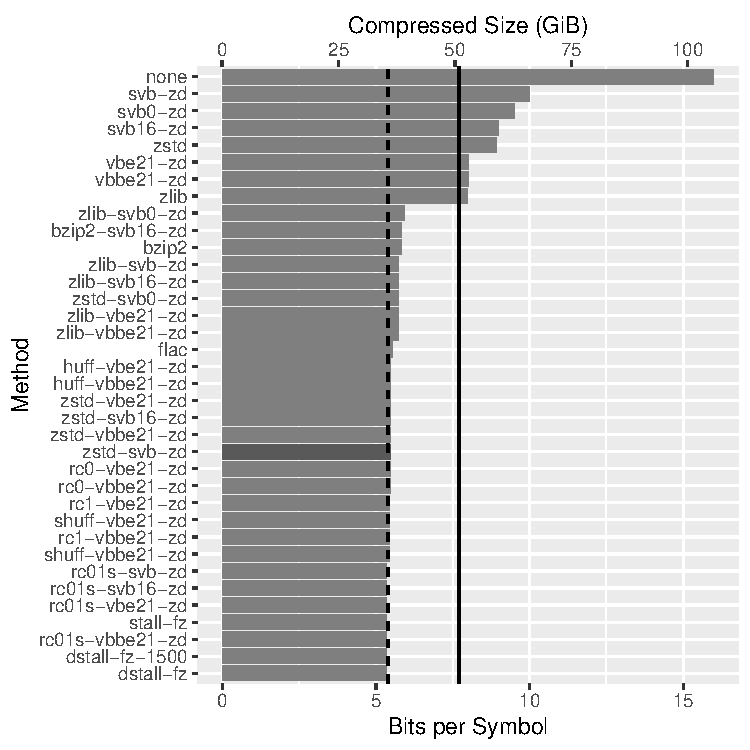
\includegraphics[scale=0.9]{plots/reads.blow5.test.bps.bar.pdf}
\caption{\label{fig:results-bps}The average number of bits used per symbol and
	total compressed size of each method on the data. The state-of-the-art
	method is highlighted in a darker grey. The solid and dotted vertical
	lines represents the bits per symbol equivalent of the entropy of the
	data and its deltas respectively.}
\end{figure}

\begin{figure}
\centering
%% Created by tikzDevice version 0.12.3.1 on 2022-11-04 11:05:01
% !TEX encoding = UTF-8 Unicode
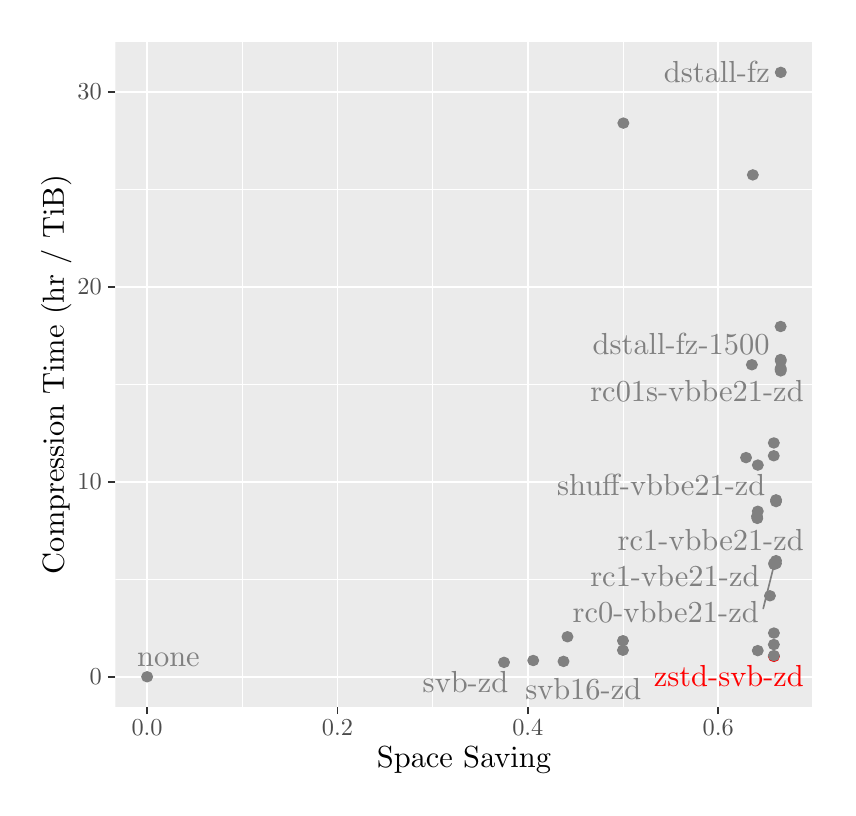
\begin{tikzpicture}[x=1pt,y=0.95pt]
\definecolor{fillColor}{RGB}{255,255,255}
\path[use as bounding box,fill=fillColor,fill opacity=0.00] (0,0) rectangle (289.08,289.08);
\begin{scope}
\path[clip] (  0.00,  0.00) rectangle (289.08,289.08);
\definecolor{drawColor}{RGB}{255,255,255}
\definecolor{fillColor}{RGB}{255,255,255}

\path[draw=drawColor,line width= 0.6pt,line join=round,line cap=round,fill=fillColor] (  0.00,  0.00) rectangle (289.08,289.08);
\end{scope}
\begin{scope}
\path[clip] ( 31.71, 30.69) rectangle (283.58,283.58);
\definecolor{fillColor}{gray}{0.92}

\path[fill=fillColor] ( 31.71, 30.69) rectangle (283.58,283.58);
\definecolor{drawColor}{RGB}{255,255,255}

\path[draw=drawColor,line width= 0.3pt,line join=round] ( 31.71, 79.26) --
	(283.58, 79.26);

\path[draw=drawColor,line width= 0.3pt,line join=round] ( 31.71,153.43) --
	(283.58,153.43);

\path[draw=drawColor,line width= 0.3pt,line join=round] ( 31.71,227.60) --
	(283.58,227.60);

\path[draw=drawColor,line width= 0.3pt,line join=round] ( 77.55, 30.69) --
	( 77.55,283.58);

\path[draw=drawColor,line width= 0.3pt,line join=round] (146.34, 30.69) --
	(146.34,283.58);

\path[draw=drawColor,line width= 0.3pt,line join=round] (215.13, 30.69) --
	(215.13,283.58);

\path[draw=drawColor,line width= 0.6pt,line join=round] ( 31.71, 42.18) --
	(283.58, 42.18);

\path[draw=drawColor,line width= 0.6pt,line join=round] ( 31.71,116.35) --
	(283.58,116.35);

\path[draw=drawColor,line width= 0.6pt,line join=round] ( 31.71,190.51) --
	(283.58,190.51);

\path[draw=drawColor,line width= 0.6pt,line join=round] ( 31.71,264.68) --
	(283.58,264.68);

\path[draw=drawColor,line width= 0.6pt,line join=round] ( 43.16, 30.69) --
	( 43.16,283.58);

\path[draw=drawColor,line width= 0.6pt,line join=round] (111.95, 30.69) --
	(111.95,283.58);

\path[draw=drawColor,line width= 0.6pt,line join=round] (180.73, 30.69) --
	(180.73,283.58);

\path[draw=drawColor,line width= 0.6pt,line join=round] (249.52, 30.69) --
	(249.52,283.58);
\definecolor{drawColor}{gray}{0.50}
\definecolor{fillColor}{gray}{0.50}

\path[draw=drawColor,line width= 0.4pt,line join=round,line cap=round,fill=fillColor] ( 43.16, 42.18) circle (  1.96);

\path[draw=drawColor,line width= 0.4pt,line join=round,line cap=round,fill=fillColor] (215.25,252.78) circle (  1.96);

\path[draw=drawColor,line width= 0.4pt,line join=round,line cap=round,fill=fillColor] (195.05, 57.40) circle (  1.96);

\path[draw=drawColor,line width= 0.4pt,line join=round,line cap=round,fill=fillColor] (262.03,233.08) circle (  1.96);

\path[draw=drawColor,line width= 0.4pt,line join=round,line cap=round,fill=fillColor] (172.13, 47.66) circle (  1.96);

\path[draw=drawColor,line width= 0.4pt,line join=round,line cap=round,fill=fillColor] (193.62, 48.03) circle (  1.96);

\path[draw=drawColor,line width= 0.4pt,line join=round,line cap=round,fill=fillColor] (182.68, 48.37) circle (  1.96);

\path[draw=drawColor,line width= 0.4pt,line join=round,line cap=round,fill=fillColor] (215.09, 52.28) circle (  1.96);

\path[draw=drawColor,line width= 0.4pt,line join=round,line cap=round,fill=fillColor] (215.10, 55.89) circle (  1.96);
\definecolor{drawColor}{RGB}{255,0,0}
\definecolor{fillColor}{RGB}{255,0,0}

\path[draw=drawColor,line width= 0.4pt,line join=round,line cap=round,fill=fillColor] (269.65, 49.93) circle (  1.96);
\definecolor{drawColor}{gray}{0.50}
\definecolor{fillColor}{gray}{0.50}

\path[draw=drawColor,line width= 0.4pt,line join=round,line cap=round,fill=fillColor] (269.64, 50.24) circle (  1.96);

\path[draw=drawColor,line width= 0.4pt,line join=round,line cap=round,fill=fillColor] (263.81, 52.13) circle (  1.96);

\path[draw=drawColor,line width= 0.4pt,line join=round,line cap=round,fill=fillColor] (269.63, 54.44) circle (  1.96);

\path[draw=drawColor,line width= 0.4pt,line join=round,line cap=round,fill=fillColor] (269.65, 58.81) circle (  1.96);

\path[draw=drawColor,line width= 0.4pt,line join=round,line cap=round,fill=fillColor] (263.53,103.18) circle (  1.96);

\path[draw=drawColor,line width= 0.4pt,line join=round,line cap=round,fill=fillColor] (263.65,102.42) circle (  1.96);

\path[draw=drawColor,line width= 0.4pt,line join=round,line cap=round,fill=fillColor] (259.58,125.54) circle (  1.96);

\path[draw=drawColor,line width= 0.4pt,line join=round,line cap=round,fill=fillColor] (263.83,105.14) circle (  1.96);

\path[draw=drawColor,line width= 0.4pt,line join=round,line cap=round,fill=fillColor] (263.84,122.70) circle (  1.96);

\path[draw=drawColor,line width= 0.4pt,line join=round,line cap=round,fill=fillColor] (261.69,160.86) circle (  1.96);

\path[draw=drawColor,line width= 0.4pt,line join=round,line cap=round,fill=fillColor] (268.22, 72.98) circle (  1.96);

\path[draw=drawColor,line width= 0.4pt,line join=round,line cap=round,fill=fillColor] (269.60,126.24) circle (  1.96);

\path[draw=drawColor,line width= 0.4pt,line join=round,line cap=round,fill=fillColor] (270.42,108.81) circle (  1.96);

\path[draw=drawColor,line width= 0.4pt,line join=round,line cap=round,fill=fillColor] (269.74, 85.41) circle (  1.96);

\path[draw=drawColor,line width= 0.4pt,line join=round,line cap=round,fill=fillColor] (270.40, 85.28) circle (  1.96);

\path[draw=drawColor,line width= 0.4pt,line join=round,line cap=round,fill=fillColor] (272.10,159.58) circle (  1.96);

\path[draw=drawColor,line width= 0.4pt,line join=round,line cap=round,fill=fillColor] (269.62,131.13) circle (  1.96);

\path[draw=drawColor,line width= 0.4pt,line join=round,line cap=round,fill=fillColor] (270.43,109.48) circle (  1.96);

\path[draw=drawColor,line width= 0.4pt,line join=round,line cap=round,fill=fillColor] (269.75, 84.94) circle (  1.96);

\path[draw=drawColor,line width= 0.4pt,line join=round,line cap=round,fill=fillColor] (270.42, 86.35) circle (  1.96);

\path[draw=drawColor,line width= 0.4pt,line join=round,line cap=round,fill=fillColor] (272.12,158.53) circle (  1.96);

\path[draw=drawColor,line width= 0.4pt,line join=round,line cap=round,fill=fillColor] (272.11,162.86) circle (  1.96);

\path[draw=drawColor,line width= 0.4pt,line join=round,line cap=round,fill=fillColor] (272.08,175.41) circle (  1.96);

\path[draw=drawColor,line width= 0.4pt,line join=round,line cap=round,fill=fillColor] (272.09,159.13) circle (  1.96);

\path[draw=drawColor,line width= 0.4pt,line join=round,line cap=round,fill=fillColor] (272.13,272.08) circle (  1.96);

\path[draw=drawColor,line width= 0.4pt,line join=round,line cap=round,fill=fillColor] (272.13,162.28) circle (  1.96);

\path[draw=drawColor,line width= 0.6pt,line join=round,line cap=round] (265.79, 68.14) -- (269.54, 84.04);

\node[text=drawColor,anchor=base,inner sep=0pt, outer sep=0pt, scale=  1.10] at ( 50.88, 46.14) {none};

\node[text=drawColor,anchor=base,inner sep=0pt, outer sep=0pt, scale=  1.10] at (158.22, 36.13) {svb-zd};

\node[text=drawColor,anchor=base,inner sep=0pt, outer sep=0pt, scale=  1.10] at (200.76, 33.70) {svb16-zd};
\definecolor{drawColor}{RGB}{255,0,0}

\node[text=drawColor,anchor=base,inner sep=0pt, outer sep=0pt, scale=  1.10] at (253.37, 38.38) {zstd-svb-zd};
\definecolor{drawColor}{gray}{0.50}

\node[text=drawColor,anchor=base,inner sep=0pt, outer sep=0pt, scale=  1.10] at (233.88, 76.64) {rc1-vbe21-zd};

\node[text=drawColor,anchor=base,inner sep=0pt, outer sep=0pt, scale=  1.10] at (228.96,111.12) {shuff-vbbe21-zd};

\node[text=drawColor,anchor=base,inner sep=0pt, outer sep=0pt, scale=  1.10] at (230.55, 62.88) {rc0-vbbe21-zd};

\node[text=drawColor,anchor=base,inner sep=0pt, outer sep=0pt, scale=  1.10] at (246.83, 90.28) {rc1-vbbe21-zd};

\node[text=drawColor,anchor=base,inner sep=0pt, outer sep=0pt, scale=  1.10] at (241.86,147.01) {rc01s-vbbe21-zd};

\node[text=drawColor,anchor=base,inner sep=0pt, outer sep=0pt, scale=  1.10] at (249.05,268.28) {dstall-fz};

\node[text=drawColor,anchor=base,inner sep=0pt, outer sep=0pt, scale=  1.10] at (236.11,164.81) {dstall-fz-1500};
\end{scope}
\begin{scope}
\path[clip] (  0.00,  0.00) rectangle (289.08,289.08);
\definecolor{drawColor}{gray}{0.30}

\node[text=drawColor,anchor=base east,inner sep=0pt, outer sep=0pt, scale=  0.88] at ( 26.76, 39.15) {0};

\node[text=drawColor,anchor=base east,inner sep=0pt, outer sep=0pt, scale=  0.88] at ( 26.76,113.32) {10};

\node[text=drawColor,anchor=base east,inner sep=0pt, outer sep=0pt, scale=  0.88] at ( 26.76,187.48) {20};

\node[text=drawColor,anchor=base east,inner sep=0pt, outer sep=0pt, scale=  0.88] at ( 26.76,261.65) {30};
\end{scope}
\begin{scope}
\path[clip] (  0.00,  0.00) rectangle (289.08,289.08);
\definecolor{drawColor}{gray}{0.20}

\path[draw=drawColor,line width= 0.6pt,line join=round] ( 28.96, 42.18) --
	( 31.71, 42.18);

\path[draw=drawColor,line width= 0.6pt,line join=round] ( 28.96,116.35) --
	( 31.71,116.35);

\path[draw=drawColor,line width= 0.6pt,line join=round] ( 28.96,190.51) --
	( 31.71,190.51);

\path[draw=drawColor,line width= 0.6pt,line join=round] ( 28.96,264.68) --
	( 31.71,264.68);
\end{scope}
\begin{scope}
\path[clip] (  0.00,  0.00) rectangle (289.08,289.08);
\definecolor{drawColor}{gray}{0.20}

\path[draw=drawColor,line width= 0.6pt,line join=round] ( 43.16, 27.94) --
	( 43.16, 30.69);

\path[draw=drawColor,line width= 0.6pt,line join=round] (111.95, 27.94) --
	(111.95, 30.69);

\path[draw=drawColor,line width= 0.6pt,line join=round] (180.73, 27.94) --
	(180.73, 30.69);

\path[draw=drawColor,line width= 0.6pt,line join=round] (249.52, 27.94) --
	(249.52, 30.69);
\end{scope}
\begin{scope}
\path[clip] (  0.00,  0.00) rectangle (289.08,289.08);
\definecolor{drawColor}{gray}{0.30}

\node[text=drawColor,anchor=base,inner sep=0pt, outer sep=0pt, scale=  0.88] at ( 43.16, 19.68) {0.0};

\node[text=drawColor,anchor=base,inner sep=0pt, outer sep=0pt, scale=  0.88] at (111.95, 19.68) {0.2};

\node[text=drawColor,anchor=base,inner sep=0pt, outer sep=0pt, scale=  0.88] at (180.73, 19.68) {0.4};

\node[text=drawColor,anchor=base,inner sep=0pt, outer sep=0pt, scale=  0.88] at (249.52, 19.68) {0.6};
\end{scope}
\begin{scope}
\path[clip] (  0.00,  0.00) rectangle (289.08,289.08);
\definecolor{drawColor}{RGB}{0,0,0}

\node[text=drawColor,anchor=base,inner sep=0pt, outer sep=0pt, scale=  1.10] at (157.65,  7.64) {Space Saving};
\end{scope}
\begin{scope}
\path[clip] (  0.00,  0.00) rectangle (289.08,289.08);
\definecolor{drawColor}{RGB}{0,0,0}

\node[text=drawColor,rotate= 90.00,anchor=base,inner sep=0pt, outer sep=0pt, scale=  1.10] at ( 13.08,157.13) {Compression Time (hr / TiB)};
\end{scope}
\end{tikzpicture}

\subfloat[\label{fig:results-ss-ct-big}]{
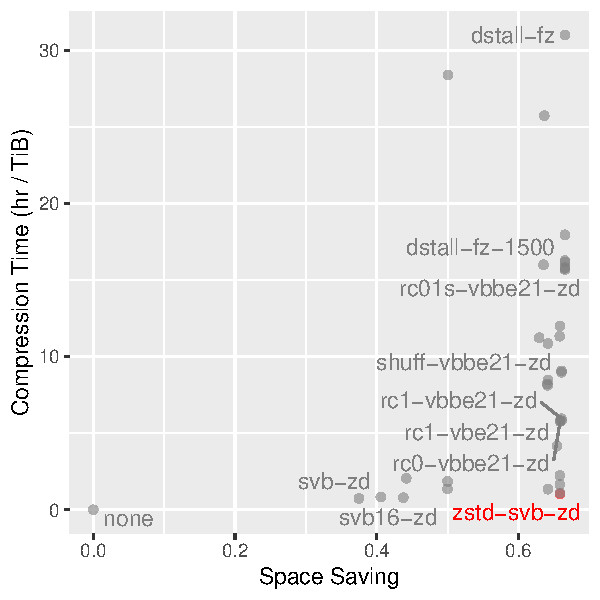
\includegraphics[scale=0.7,valign=t]{plots/reads.blow5.test.ss-ct.pdf}
}
\subfloat[\label{fig:results-ss-ct-small}]{
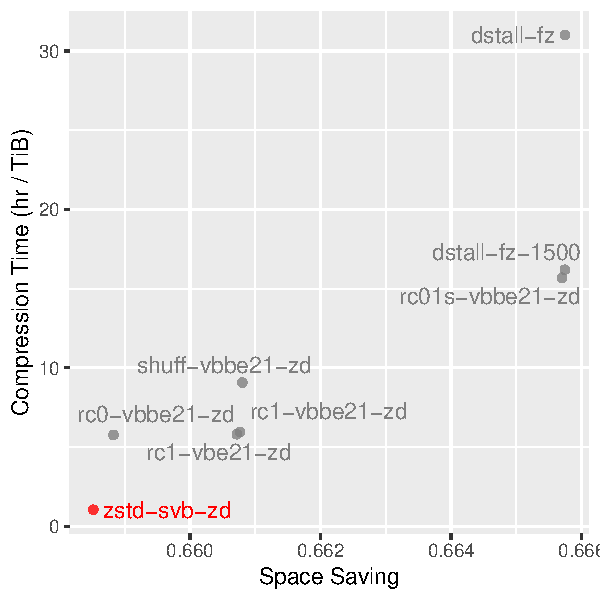
\includegraphics[scale=0.7,valign=t]{plots/reads.blow5.test.ss-ct06.pdf}
}

\subfloat[\label{fig:results-ss-dt-big}]{
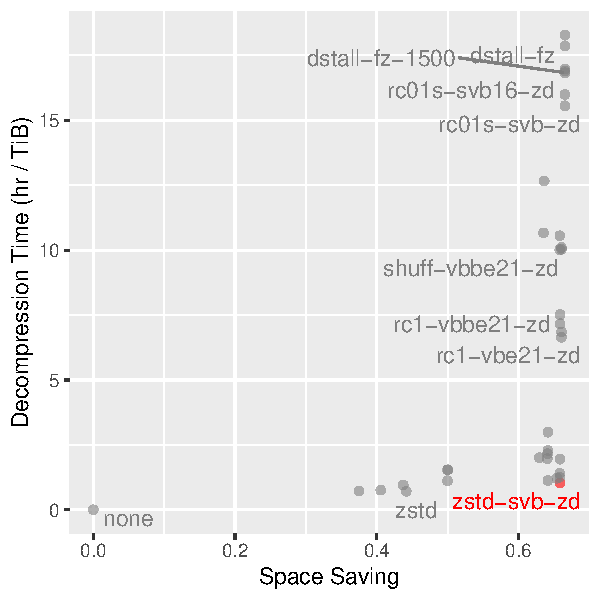
\includegraphics[scale=0.7,valign=t]{plots/reads.blow5.test.ss-dt.pdf}
}
\subfloat[\label{fig:results-ss-dt-small}]{
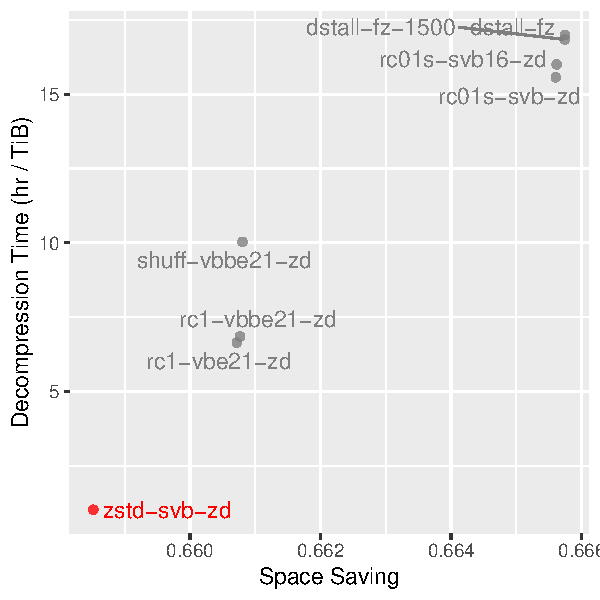
\includegraphics[scale=0.7,valign=t]{plots/reads.blow5.test.ss-dt06.pdf}
}
\caption{\label{fig:results-ss-t}The (de)compression time (in hours per TiB)
	versus space saving of various methods. The state-of-the-art method is
	coloured in red and the labelled methods are on the
	space--(de)compression-time frontier. That is, for each labelled method
	in Figures \ref{fig:results-ss-ct-big} and
	\ref{fig:results-ss-ct-small}
	there is no other compression method which produces a greater space
	saving in less time. Whilst for each labelled method in Figures
	\ref{fig:results-ss-dt-big} and \ref{fig:results-ss-dt-small} there is
	no other compression method which has a greater space saving and
	decompresses in less time.
	Figures \ref{fig:results-ss-ct-big} and \ref{fig:results-ss-dt-big} show all the
	methods. Whilst Figures \ref{fig:results-ss-ct-small} and
	\ref{fig:results-ss-dt-small} show the methods which are on their
	respective froniter and have a space saving greater than or equal to the
	state-of-the-art.}
\end{figure}

\begin{figure}
\centering
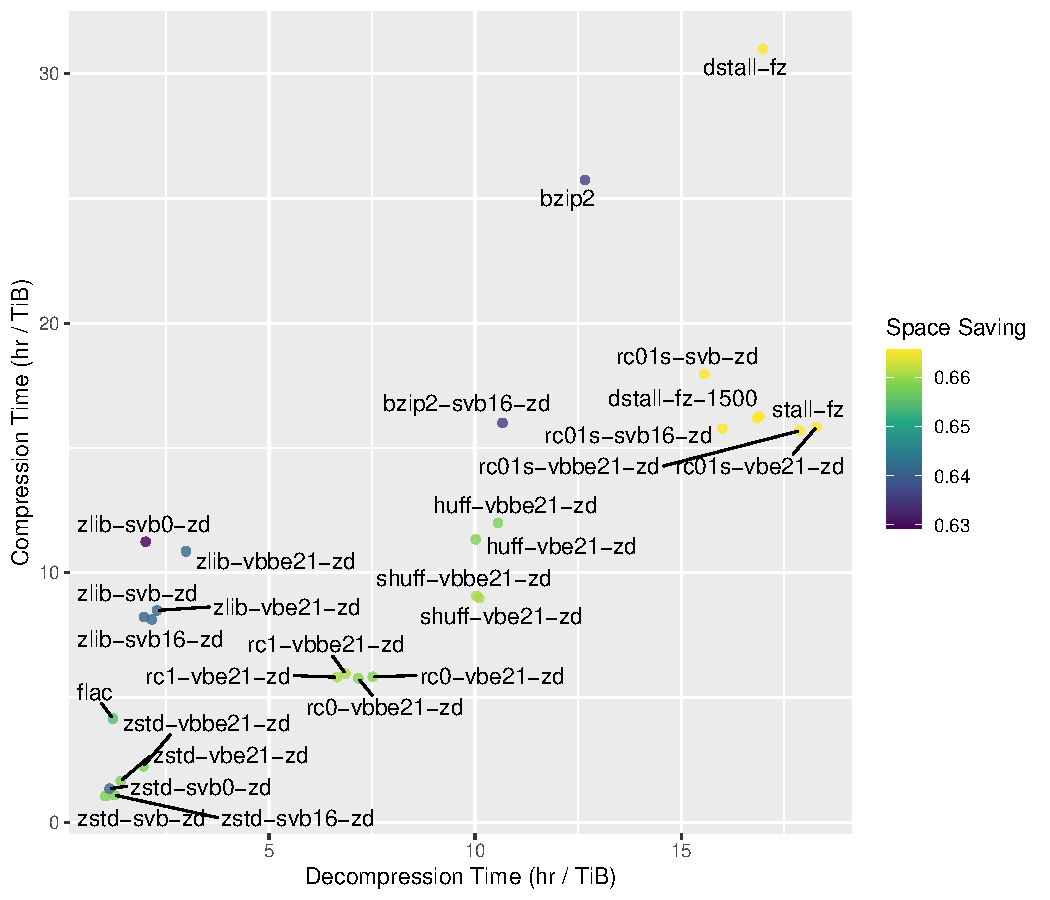
\includegraphics[scale=0.7]{plots/reads.blow5.test.ct-dt.pdf}
	\caption{\label{fig:results-ct-dt}A scatter plot of the methods which
	have a space saving greater than or equal to the state-of-the-art.
	Compression time is plotted against decompression time (in hours per
	TiB) and each point is coloured by its space saving. The
	state-of-the-art method zstd-svb-zd is in the bottom-left corner.}
\end{figure}


%\begin{table}
    \caption{\label{tab:vbz} Performance results on the data set using only one thread of execution.}
	\begin{tabular}{|l|l|}
        \hline
Compression Ratio & 2.93\\
		Compression Speed (mins per TiB) & 62.5\\

		Decompression Speed (mins per TiB) & 61.5\\
	\hline
    \end{tabular}
\end{table}

